% \iffalse meta-comment
%<*internal>
\begingroup
\input docstrip
\preamble

The 'suftesi' document class 
Copyright (C) 2009-2021 Ivan Valbusa
<ivan dot valbusa at gmail dot com>

All rights reserved.

This work may be distributed and/or modified under the
conditions of the LaTeX Project Public License, either version 1.3
of this license or (at your option) any later version. 
The latest version of this license is in
   http://www.latex-project.org/lppl.txt
and version 1.3 or later is part of all distributions of LaTeX
version 2005/12/01 or later.

This work consists of all files listed in README

This work has the LPPL maintenance status "author-maintained".

\endpreamble
\keepsilent
\askforoverwritefalse

\Msg{*** Generating the class file ***}
\generate{
  \file{suftesi.cls}{\from{suftesi.dtx}{class}}
  \nopreamble\nopostamble
  \file{suftesi.bib}{\from{suftesi.dtx}{bib}}} 

\Msg{***********************************************************}
\Msg{*}
\Msg{* To finish the installation you have to move the following}
\Msg{* files into a directory searched by TeX:}
\Msg{*}
\Msg{* \space\space suftesi.cls}
\Msg{*}
\Msg{*}
\Msg{* To produce the documentation on suftesi's code run}
\Msg{* the file ending with `.dtx' through (pdf)LaTeX. See the}
\Msg{* README file for more details.}
\Msg{*}
\Msg{* Happy TeXing}
\Msg{***********************************************************}
\endgroup
%</internal>
% \fi
% \iffalse
%<*driver>
\ProvidesFile{suftesi.dtx}
%</driver>
%<class>\NeedsTeXFormat{LaTeX2e}[2005/12/01]
%<class>\ProvidesClass{suftesi}
%<*class>
    [2021/11/01 v3.2.0 A class for typesetting theses, books and articles]
%</class>
%<*driver>
\documentclass[12pt]{ltxdoc}
\usepackage[T1]{fontenc}
\usepackage[utf8]{inputenc}
\usepackage[fontsize=12pt]{fontsize}
\usepackage[greek.ancient,english]{babel}
\usepackage{afterpage}
%--------------------------------------------------------
% GRAPHICS
%--------------------------------------------------------
\usepackage[svgnames]{xcolor}
\definecolor{philA}{named}{DarkRed}
\definecolor{philB}{named}{NavyBlue}
\definecolor{sufred}{rgb}{0.5,0,0}
\definecolor{sufgray}{rgb}{0.5,0.5,0.5}
\usepackage{tikz}
  \usetikzlibrary{shadows,patterns}
  \tikzset{
    pframe/.style={draw=gray,fill=white,drop shadow},
    pnode/.style={anchor=north west,align=justify,text width=.85\textwidth}}
\usepackage[framemethod=TikZ]{mdframed}
  \mdfsetup{roundcorner=3pt,linecolor=white,backgroundcolor=gray!10}
%--------------------------------------------------------
% DOC FACILITIES
%--------------------------------------------------------
\usepackage{hologo}
\usepackage{guit}% before ltxdockit but after xcolor!
\usepackage[final]{microtype}
\let\cs\relax
\let\cmd\relax
\usepackage{ltxdockit}
%--------------------------------------------------------
% FONTS
%--------------------------------------------------------
\usepackage{cochineal}
% To use the cochineal inside the document we have to define the family
% because the .fd files of the font refer to conditionals 
% defined in 'cochineal.sty’:
\DeclareFontFamily{T1}{Cochineal-LF}{}
\DeclareFontShape{T1}{Cochineal-LF}{m}{n}{
  <-> s*[1.0] Cochineal-Roman-osf-t1}{}
\usepackage[varqu,varl,var0]{inconsolata}
\usepackage{biolinum}
\usepackage{amsthm}
\usepackage[cochineal,bigdelims,cmintegrals,vvarbb]{newtxmath}
\usepackage[cal=boondoxo]{mathalpha}
\usepackage{manfnt}
%--------------------------------------------------------
% LAYOUT
%--------------------------------------------------------
\usepackage[skip=1.5ex]{parskip}
\usepackage{geometry}
\geometry{
  a4paper,
  margin=3cm,
  headheight=15pt,
  ignoreall,
  heightrounded}
\usepackage{sectsty}
\allsectionsfont{\sffamily}
% --------------------------------------------------------
% OTHER PACKAGES
% --------------------------------------------------------
\usepackage[autostyle]{csquotes}
\usepackage[style=philosophy-classic]{biblatex}
\addbibresource{suftesi.bib}
\DeclareBibliographyCategory{pkgs-loaded}
\addtocategory{pkgs-loaded}{appendix,caption,color,crop,enumitem,emptypage,
fancyhdr,fixltxhyph,fontsize,mathalpha,libertinust1math,newtx,geometry,
iftex,microtype,multicol,titlesec,titletoc,xkeyval,cclicenses,
substitutefont,luatex85,lm,textcomp,newpx,biolinum,inconsolata,libertine,
cochineal,mathpazo,bera,amsthm}
\usepackage{array}
\usepackage{booktabs}
\usepackage{multirow}
\usepackage{siunitx}
%--------------------------------------------------------
% COMMANDS AND ENVIRONMENTS
%--------------------------------------------------------
\newcommand{\new}{\marginpar{\textcolor{red}{\textbf{NEW!}}}}
\newcommand{\argstyle}{\itshape}
\DeclareRobustCommand*{\ar}[1]{\texttt{\char`\{}\textrm{\argstyle#1}\texttt{\char`\}}}
\DeclareRobustCommand*{\oar}[1]{\texttt{[}\textrm{\argstyle#1}\texttt{]}}
\DeclareRobustCommand*{\meta}[1]{%
  $\langle${\argstyle\rmfamily#1\kern0.12em}$\rangle$}
\DeclareRobustCommand*{\arm}[1]{\ar{\meta{\argstyle#1}}}
\DeclareRobustCommand*{\oarm}[1]{\oar{\meta{\argstyle#1}}}
\newcommand*{\OR}{${}\mid{}$}
\makeatletter
\newlength\CLett
\newcommand*\alert{
 \par\noindent
 \setbox\z@\hbox{\textdbend}\CLett=\wd\z@%
 \raisebox{-1.05\baselineskip}[0pt][0pt]{%
  \llap{\box\z@\kern6pt}}} 
\makeatother
% New environments
\newenvironment{ttquote}{%
  \begin{mdframed}\ttfamily\microtypesetup{activate=false}}{\end{mdframed}}
\newenvironment{latexcode}{\begin{mdframed}}{\end{mdframed}}
\makeatletter
% Customizing option and value list:
\renewcommand*{\ltd@ol@optitem}[3][]{%To use \meta inside #2
  \ifblank{#1}
  {\ltd@option{}{#2}{#3}{}}
  {\ltd@option{}{#2}{#3}{\ltd@textverb{#1}}}}%
\pretocmd{\valuelist}{\let\optionlistfont\valuelistfont}{}{}
\patchcmd{\ltxsyntax}{\marglistwidth}{0pt}{}{}
\patchcmd{\ltd@option@i}{=}{\ = }{}{}
\patchcmd{\ltd@option@ii}{=}{\ = }{}{}
\expandafter\patchcmd\csname\string\valuelist\endcsname{{\leftmargin}{\labelsep}}{{\leftmargin}{3\labelsep}}{}{}
% New color for items
\newcommand*{\valuelistfont}{%
  \color{olive}\sffamily\displayverbfont}
\renewcommand*{\optionlistfont}{%
  \color{philA}\sffamily\displayverbfont}
\renewcommand*{\ltxsyntaxlabelfont}{%
  \color{philA}\sffamily\displayverbfont}
\renewcommand*{\marglistfont}{%
  \color{philA}\sffamily\displayverbfont}
% Table of contents
\renewcommand\tableofcontents{%
  \setlength{\columnsep}{1cm}
  {\centering      
    \section*{\contentsname}%
    \@mkboth{\contentsname}{\contentsname}}   
  \thispagestyle{empty}
  \begin{multicols}{2}
    \@starttoc{toc}%
\end{multicols}}
\makeatother
% --------------------------------------------------------
% GREEK EXAMPLES
% --------------------------------------------------------
\makeatletter
\newcommand{\mygrsize}{\f@size}
\makeatother
\newcommand{\mygrpxsize}{12.5}
\def\latintxt{Aliquam auctor, pede consequat
  laoreet varius, eros tellus maris quam, pellentesque hendrerit.
  Verecundia conditur.}  
\def\latintxtb{Morbi luctus, wisi viverra faucibus pretium,
  nihil est placerat pro cuius loquentis verba. Sed maleficium in quibusdam certum.}
\def\greektxt{Πρῶτον εἰπεῖν περὶ τί καὶ τίνος ἐστὶν ἡ σκέψις, ὅτι περὶ 
ἀπόδειξιν καὶ ἐπιστήμης ἀποδεικτικῆς· εἶτα διορίσαι τί 
ἐστι πρότασις καὶ τί ὅρος καὶ τί συλλογισμός}    
\newcommand{\greekexample}[4]{%
  \noindent\textbf{#3}{ \fontfamily{#1}\selectfont\latintxt\ }% 
    {\fontfamily{#2}\fontsize{#4}{13}\selectfont%
    \textgreek{\greektxt}} {\fontfamily{#1}\selectfont\latintxtb}\par\vskip 6pt plus 1pt minus 1pt}
% --------------------------------------------------------
% LAYOUTS THUMBNAILS
% --------------------------------------------------------
\usepackage{xfp}
\NewExpandableDocumentCommand{\sufgetlength}{O{pt}mm}{%
  % #1 (optional, default pt), #2 = length
  \fpeval{round((#3)/(1#1),#2)}}
\newlength{\expaperwidth}
\newlength{\expaperheight}
\newlength{\extextwidth}
\newlength{\extextheight}
\newlength{\exxshift}
\newlength{\exyshift}
\newlength{\exzshift}
\def\sufsetlengthsA{%marginratio: 2/3
  \setlength{\exxshift}{\dimexpr(0.666\expaperwidth-0.666\extextwidth)}
  \setlength{\exyshift}{\dimexpr(0.666\expaperheight-0.666\extextheight)}
  \setlength{\exzshift}{\dimexpr(2\expaperwidth-\extextwidth-\exxshift)}}
\def\sufsetlengthsB{%marginratio: 1/1
  \setlength{\exxshift}{\dimexpr(0.5\expaperwidth-0.5\extextwidth)}
  \setlength{\exyshift}{\dimexpr(0.5\expaperheight-0.5\extextheight)}
  \setlength{\exzshift}{\dimexpr(2\expaperwidth-\extextwidth-\exxshift)}}
\def\sufsetlengthsC{%hmarginratio: 1/1; vmarginratio:2/3
  \setlength{\exxshift}{\dimexpr(0.5\expaperwidth-0.5\extextwidth)}
  \setlength{\exyshift}{\dimexpr(0.666\expaperheight-0.666\extextheight)}
  \setlength{\exzshift}{\dimexpr(2\expaperwidth-\extextwidth-\exxshift)}}
\newcommand{\sufpagesetup}[6]{%
  \setlength{\extextwidth}{#3cm}%
  \setlength{\extextheight}{#4cm}%
  \setlength{\expaperwidth}{#5cm}%
  \setlength{\expaperheight}{#6cm}%
  \sufsetlengths%
  \tikzset{body/.style ={yshift=\exyshift,draw=none,pattern={horizontal lines light gray}}}%
  \tikzset{page/.style ={fill=gray!5!yellow!2,draw=gray!50}}%
  \begin{tikzpicture}[scale=#1]
  \draw[page] (0,0) rectangle (\expaperwidth,\expaperheight);
  \draw[page,xshift=\expaperwidth] (0,0) rectangle (\expaperwidth,\expaperheight);
  \draw[draw=gray!10,thick] (\expaperwidth,0) -- (\expaperwidth,\expaperheight);
  \draw[xshift=\exxshift,body] (0,0) rectangle (\extextwidth,\extextheight);
  \draw[xshift=\exzshift,body] (0,0) rectangle (\extextwidth,\extextheight);
  \node at (\expaperwidth,-4) (caption) {\parbox{3cm}{\centering\footnotesize\texttt{#2}\par (\sufgetlength[cm]{2}{\expaperwidth} $\times$ \sufgetlength[cm]{2}{\expaperheight})\par}};
  \end{tikzpicture}}
% --------------------------------------------------------
% OTHER THUMBNAILS
% --------------------------------------------------------
\def\shortlipsum{The phenomena should only be used as a canon for our understanding. }
\newcommand{\fakechapter}[1]{%
  \noindent
  \begin{minipage}{.31\textwidth}
    \begin{tikzpicture}
      \draw[pframe] (0,0) rectangle (\textwidth,3.8);
      \node[pnode] at (0.25,3.7) 
        {\begingroup#1\par\vspace{2\baselineskip}\endgroup
        \tiny\shortlipsum\shortlipsum\shortlipsum\shortlipsum\par};
    \end{tikzpicture}
  \end{minipage}
}
\newcommand{\fakefootnote}[1]{%
 \def\thempfootnote{\tiny 7}
  \noindent
  \begin{minipage}{.49\textwidth}
    #1\footnotesize%
    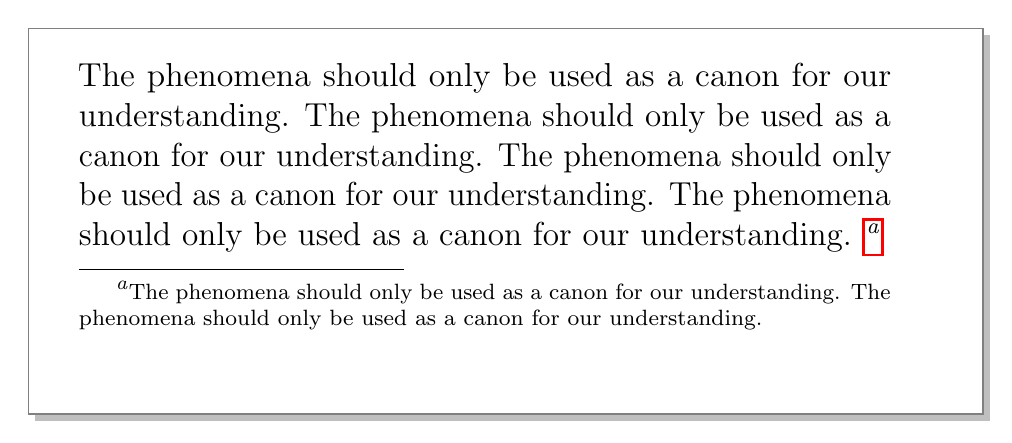
\begin{tikzpicture}
      \draw[pframe] (0,0) rectangle (\textwidth,4.9);
      \node[pnode] at (0.5,4.6)
        {\shortlipsum\shortlipsum\shortlipsum\shortlipsum%
        \footnote{\scriptsize\shortlipsum\shortlipsum\par}};
    \end{tikzpicture}%
  \end{minipage}
}
\newcommand{\fakelist}[1]{%
  \noindent
  \begin{minipage}{.31\textwidth}
    \footnotesize
    \begin{tikzpicture}
      \draw[pframe] (0,0) rectangle (\textwidth,3.3);
      \node[pnode] at (0.3,3.2) 
        {\shortlipsum:%
        \begin{list}{\color{gray}\textbullet}{\leftmargin=#1\itemsep=0pt}
        \item immagination
        \item experience
        \item emotions
        \end{list}};
    \end{tikzpicture}%
  \end{minipage}
}
\newcommand{\fakequotation}[1]{%
  \noindent
  \begin{minipage}{.31\textwidth}
    \fontsize{9}{10.5}\selectfont%
    \begin{tikzpicture}
        \draw[pframe] (0,0) rectangle (\textwidth,7);
         \node[pnode] at (0.25,6.8) 
         {\hskip1em\shortlipsum\shortlipsum\smallskip
         \begin{list}{}{#1}
          \item \fontsize{7}{8.5}\selectfont\shortlipsum\shortlipsum\shortlipsum\shortlipsum
         \end{list}\smallskip
         \hskip1em\shortlipsum\shortlipsum};
    \end{tikzpicture}%
  \end{minipage}
}
% --------------------------------------------------------
% HYPERREF SETUP
% --------------------------------------------------------
\usepackage{hyperref}
\hypersetup{%
  hidelinks,
  pdftitle={User's guide to \textsf{suftesi}},
  pdfsubject={A document class for typesetting theses, 
    books and articles},
  pdfauthor={Ivan Valbusa},
  pdfkeywords={thesis, humanities, books}}   
% --------------------------------------------------------
% FINAL SETTINGS
% --------------------------------------------------------
\setcounter{tocdepth}{2}
\widowpenalty=10000
\clubpenalty=10000

\EnableCrossrefs         
\CodelineIndex
\RecordChanges

\begin{document}
  \DocInput{suftesi.dtx}
\end{document}
%
%</driver>
% \fi
%
% \CheckSum{5685}
%
% \CharacterTable
%  {Upper-case    \A\B\C\D\E\F\G\H\I\J\K\L\M\N\O\P\Q\R\S\T\U\V\W\X\Y\Z
%   Lower-case    \a\b\c\d\e\f\g\h\i\j\k\l\m\n\o\p\q\r\s\t\u\v\w\x\y\z
%   Digits        \0\1\2\3\4\5\6\7\8\9
%   Exclamation   \!     Double quote  \"     Hash (number) \#
%   Dollar        \$     Percent       \%     Ampersand     \&
%   Acute accent  \'     Left paren    \(     Right paren   \)
%   Asterisk      \*     Plus          \+     Comma         \,
%   Minus         \-     Point         \.     Solidus       \/
%   Colon         \:     Semicolon     \;     Less than     \<
%   Equals        \=     Greater than  \>     Question mark \?
%   Commercial at \@     Left bracket  \[     Backslash     \\
%   Right bracket \]     Circumflex    \^     Underscore    \_
%   Grave accent  \`     Left brace    \{     Vertical bar  \|
%   Right brace   \}     Tilde         \~}
%
% \changes{v3.2.0}{2021/11/01}{Fixed a bug in \cmd{xfootnote} command. 
% Fixed a bug occurring when using the \cmd{geometry} command.}
% \changes{v3.1.3}{2021/06/06}{Maintenance release. 
% Moved commands for breaking titles after \opt{titletoc} settings. 
% Corrected a bug in \cmd{maketitle} with the \opt{collection} structure. 
% Added \sty{etoolbox}, previously removed by mistake.}
% \changes{v3.1.2}{2021/06/05}{Corrected a bug with \opt{reverseauthortitle} option.}
% \changes{v3.1.1}{2021/05/23}{Redefined some boolean options. Renamed some private commands. Corrected a bug in headers numbering (\cmd{protect} removed). Disabled automatic partial ToC functionality. Improved \opt{fewfootnotes} option via \sty{zref}. Updated documentation.}
% \changes{v3.1.0}{2021/05/20}{Replaced \cmd{val}\cmd{nr} with \cmd{suftesi@val}\cmd{suftesi@nr}. Corrected a bug with \cmd{maketitle} in \opt{collection} structure. New options \opt{partialtoc} and \opt{maketitlestyle}. New commands for customizing the partial ToC. New value \opt{justify} for \opt{quotestyle} option. Improved \opt{quotesize} option. Renamed the \opt{revauthortitle} option to \opt{reverseauthortitle}. The options \opt{titlefont}, \opt{authorfont}, \opt{reverseauthortitle} now work for every structure. Renewed documentation}
% \changes{v3.0.2}{2021/02/06}{Improved \opt{subsecstyle} and \opt{subsubsecstyle} options.}
% \changes{v3.0.1}{2021/01/27}{Maintenance release.}
% \changes{v3.0}{2021/01/24}{Improved \sty{biblatex} support. Updated documentation.}
% \changes{v2.9.9b (2.9.11)}{2020/12/21}{New page layouts: \opt{pocketa}, \opt{pocketb}, \opt{pocketc}. New commands \cmd{breakinbody}, \cmd{breakinbodyleft}, \cmd{breakintoc} (old names: \cmd{headbreak} and \cmd{xheadbreak}). Changed definitions of \cmd{appendixpagename}, \cmd{appendixtocname} and \cmd{appendixname} commands (default: english). The \cmd{part} command has been completely redefined. Updated documentation.}
% \changes{v2.9.9a (2.9.10)}{2020/06/26}{Corrected a bug using the \env{otherlanguage} environment with \opt{greekfont} option. Updated documentation.}
% \changes{v2.9.9}{2020/05/21}{Removed a bug with \cmd{appendix} and roman chapter numbers in table of contents. Updated documentation.}
% \changes{v2.9.8}{2020/02/24}{Removed license restrictions. Updated documentation.}
% \changes{v2.9.7}{2020/02/22}{New option \opt{fontsize}. The \opt{parindent} options now accepts arbitrary values. Updated documentation.}
% \changes{v2.9.6a}{2020/02/11}{Maintenance release}
% \changes{v2.9.6}{2020/02/10}{New option \opt{compacttoc}. The appendix page title is printed in the font of the chapters by default. Removed \cmd{apepndicesname} command.}
% \changes{v2.9.5}{2020/02/04}{Restored \texttt{templates} folder. New template \texttt{book-customize}. New mechanism for the appendices through the \sty{appendix} package.}
% \changes{v2.9.4}{2020/01/01}{Updated documentation.}
% \changes{v2.9.3}{2020/01/29}{Updated documentation.}
% \changes{v2.9.2}{2019/10/26}{Added \cmd{protect} to \cmd{SUF@thechapter} and \cmd{SUF@thesection} in the definitions of \cmd{chaptermark} and \cmd{sectionmark} to correct a bug when loading \texttt{greek} option with \sty{babel}}
% \changes{v2.9.1}{2018/11/09}{Added \sty{libertinust1math} package for Libertine font. Added \sty{luatex85} for Lua\TeX{} engine}
% \changes{v2.9}{2016/04/04}{New options \opt{tocauthorfont} and \opt{toctitlefont}. Added macros\cmd{suftesi@MakeTextTOCLowercase} and \cmd{SUF@TOCtitlesmallcaps}. Improved \cmd{xheadbreak} command. New templates \texttt{book}, \texttt{theses-template-article}, \texttt{theses-template-book}.}
% \changes{v2.8}{2016/03/30}{\sty{textcase} no longer loaded. Changed definitions of \cmd{suftesi@MakeTextLowercase}, \cmd{SUF@titlesmallcaps}, \cmd{headbreak}, \cmd{xheadbreak}.}
% \changes{v2.7.1}{2016/03/22}{Corrected a bug in v.2.7 (missing some \cmd{fi} commands).}
% \changes{v2.7}{2016/03/22}{New value \opt{cscreen} for \opt{version} option. Updated documentation. Removed value \opt{elements} for options:\opt{pagelayout}, \opt{headerstyle}, \opt{captionstyle}, \opt{chapstyle}, \opt{style}; \opt{sufelements} for  option: \opt{style}. The \cmd{chapnumfont} command is no longer available.}
% \changes{v2.6}{2016/03/13}{New \opt{mathfont} option for non-standard fonts. New command \cmd{makecover} for printing the cover page. Updated documentation.}
% \changes{v2.5}{2016/03/02}{Corrected a bug when loading CB Greek fonts. Renamed option \opt{documentstructure} to \opt{structure}.  Updated documentation.}
% \changes{v2.4}{2016/02/27}{Changed the default font to Cochineal with Linux Biolinum sans serif and Inconsolata monospaced. The Palatino is now loaded with \sty{newpxtext} and \sty{newpxmath}. Bera Mono and Iwona have been substituted by Linux Biolinum and Inconsolata. New values for font options: \opt{cochineal}, \opt{libertine}, \opt{bodoni} (greek only). Value \opt{compatibility} for \opt{defaultfont} option to get the fonts of suftesi v2.3 or previous. Updated documentation.}
% \changes{v2.3}{2015/09/19}{Maintenance release.}
% \changes{v2.2}{2015/09/10}{Maintenance release.}
% \changes{v2.1}{2015/06/13}{New option \opt{toc\meta{level}font}. Updated documentation. Removed \cmd{includeart} command}
% \changes{v2.0.1}{2015/03/31}{Corrected a bug in \opt{version} option.}
% \changes{v2.0}{2015/03/29}{New page layout \opt{standardaureo}. Enhanced support for Lua\LaTeX. Headers settings are now executed \cmd{AtBeginDocument}. Loaded \sty{ifluatex} and \sty{ifthen} packages. Added \opt{listparindent} to \cmd{setlist} options. Updated documentation.}
% \changes{v1.9c}{2014/04/05}{The \opt{cbgreek} value for the \opt{greekfont} option allows now to use the full set of the CB Greek font together with the default font (Palatino).}
% \changes{v1.9b}{2014/02/16}{Corrected a bug in ``toc'', ``lof'' and ``lot'' commands.}
% \changes{v1.9a}{2014/02/11}{Maintenance release. Updated greek support. Updated documentation.}
% \changes{v1.9}{2013/09/21}{Added \opt{italic}, \opt{smallcaps} and \opt{sanserif} values for \opt{captionstyle} option. New \opt{twocolcontents} option. New \opt{supercompactaureo} page layout. Changed \cmd{toclabelspace} command and renamed to \cmd{toclabelwidth}. New \opt{collection} document structure}
% \changes{v1.8}{2013/07/18}{Maintenance release. Corrected a bug in the definition of \cmd{appendix}}
% \changes{v1.7}{2013/06/20}{Renamed \opt{viewmode} option to \opt{version}:  
% renamed \opt{print} value to \opt{draft} and 
% added \opt{final} value. New \opt{smallcapsstyle} option.}
% \changes{v1.6}{2013/04/17}{New option \opt{viewmode}. Corrected bugs in the definition of \cmd{listoffigures}, \cmd{listoftables} and \cmd{tableofcontens} commands. Updated documentation.}
% \changes{v1.5}{2013/03/22}{The \sty{microtype} package is loaded for all engines. Improved compatibility with \sty{todonotes} package and with \sty{mdframed} and \sty{bookmark} packages when using \sty{style} class option. New option \opt{viewmode}}
% \changes{v1.4}{2013/03/15}{New value \opt{periodicalaureo} for option \opt{pagelayout}. Changed code for \cmd{xfootnote} command.}
% \changes{v1.3}{2013/03/05}{Updated documentation. Added \opt{FSPLa}, 
% \opt{FSPLb} and \opt{FSPLc} styles.}
% \changes{v1.2}{2012/10/24}{Maintenance release. Added the 
% \cmd{toclabelspace} command.}
% \changes{v1.1}{2012/10/20}{Added the \sty{fixltxhyph} package. 
% Documentation updated.}
% \changes{v0.9c}{2012/09/25}{Maintenance release, no changes}
% \changes{v0.9b}{2012/09/23}{Restored \opt{11pt} and \opt{12pt} option 
% to default}
% \changes{v0.9a}{2012/08/31}{Added \option{inline} option to 
% \sty{enumitem} package. Deleted \opt{centertitle} option. 
% Deleted \opt{sctitles} option. 
% Changed code for toc, lot and lof elements.}
% \changes{v0.9}{2012/04/22}{Improved compatibility 
% with \sty{mathspec}}
% \changes{v0.8}{2012/03/19}{Added macro for using \sty{frontespizio} 
% package with \opt{compact} and \opt{supercompact} options.}
% \changes{v0.7}{2011/02/05}{Maintenance release, no changes. 
% Provided a thesis template}
% \changes{v0.6c}{2011/11/16}{Maintenance release, no changes}
% \changes{v0.6b}{2011/11/07}{Improved full compatibility with 
% Xe\LaTeX. 
% \sty{varioref} and \sty{footmisc} packages are no longer loaded}
% \changes{v0.6a}{2011/10/24}{Maintenance release, no changes}
% \changes{v0.6}{2011/10/21}{English documentation. Renamed options 
% \opt{plain} and \opt{fullplain} to \opt{centerheadings} 
% and \opt{sufplain}.}
% \changes{v0.5}{2011/10/21}{First public release. 
% The frontispiece of \sty{suftesi}{} is now
% included in the package \sty{frontespizio}. 
% New option \opt{fullplain} 
% Changed option \opt{sctitles}.}
% \GetFileInfo{suftesi.dtx}
%
% \DoNotIndex{\hskip,\newcommand,\newenvironment,\def,\begin,\vskip,\ }
% \DoNotIndex{\DeclareOption,\ExecuteOptions,\RequirePackage}
% \DoNotIndex{\@@end,\@empty,\@ifclassloaded,\@nameuse,\@nil}
% \DoNotIndex{\@undefined,\\,\`,\addtocounter,\advance,\bfseries}
% \DoNotIndex{\centering,\closeout,\define@key,\documentclass}
% \DoNotIndex{\edef,\else,\end,\endinput,\endtitlepage,\expandafter}
% \DoNotIndex{\extracolsep,\fi,\fill,\fontsize,\g@addto@macro,\toks}
% \DoNotIndex{\hrule,\hspace,\if,\if@twoside,\ifcase,\ifdefined}
% \DoNotIndex{\iffalse,\IfFileExists,\ifnum,\ifx,\immediate}
% \DoNotIndex{\jobname,\let,\long,\MakeUppercase,\MessageBreak}
% \DoNotIndex{\newcount,\newif,\newpage,\newtoks,\newwrite,\next}
% \DoNotIndex{\noexpand,\nofiles,\normalfont,\normalsize,\null}
% \DoNotIndex{\openout,\or,\styage,\styageError,\styageWarning}
% \DoNotIndex{\styageWarningNoLine,\paperheight,\paperwidth,\par}
% \DoNotIndex{\parbox,\parindent,\relax,\scshape,\selectfont,\setkeys}
% \DoNotIndex{\sffamily,\space,\stretch,\string,\textheight,\textwidth}
% \DoNotIndex{\the,\thispagestyle,\unexpanded,\unless,\unskip,\upshape}
% \DoNotIndex{\usepackage,\vbox,\vfill,\vfil,\vspace,\write,\z@}
% \DoNotIndex{\addvspace,\setcounter,\addcontentsline}
% \DoNotIndex{\filleft,\filcenter,\filright,\geometry}
% \DoNotIndex{\CurrentOption,\AtEndDocument,\@ne,\c@page,\m@ne}
% \DoNotIndex{\@firstofone,\@gobble,\@makeother,\begingroup,\endgroup}
% \DoNotIndex{\eTeXversion,\hbox,\hsize,\includegraphics,\newlinechar}
% \DoNotIndex{\titlepage,\vss,\vtop,\xdef,\@gobbletwo,\color,\dimexpr}
% \DoNotIndex{\huge,\large,\makebox,\ProcessOptions,\renewcommand}
%
%\nocite{appendix,caption,color,crop,enumitem,emptypage,fancyhdr,fixltxhyph,fontsize,mathalpha,libertinust1math,newtx,geometry,iftex,microtype,multicol,titlesec,titletoc,xkeyval,cclicenses,substitutefont,luatex85,lm,textcomp,newpx,biolinum,inconsolata,libertine,cochineal,mathpazo,bera,amsthm,zref,etoolbox}
%
% \thispagestyle{empty}
%
% \begin{tikzpicture}[overlay,remember picture]
% \draw[circular drop shadow,draw=none,fill=white] (current page.center) circle (6cm) node[align=center,anchor=center] {%
% Ivan Valbusa\\[1cm]
% 
%\Huge\color{gray}\bfseries \parbox{10cm}{\centering The \\{{\color{philA}\fontsize{30}{32}\textsf{suftesi}}\\ document class}}\\[1cm]
% \color{black!60!Goldenrod}
%
%\normalsize \fileversion{} -- \filedate
% 
%};
% \end{tikzpicture}
% \clearpage\thispagestyle{empty}
% \null\vspace{1cm}
%
%\hfill\begin{minipage}{.5\textwidth}
% \raggedleft\footnotesize
% The serif typeface is Cochineal, created by Michael Sharpe 
% on the basis of Sebastian Kosch's Crimson. 
% The \texttt{typewriter} font is Inconsolata, 
% designed by Raph Levien and the \textsf{sans serif} text 
% is typeset in Linux Biolinum, created by Philipp H.~Poll. 
%\end{minipage}
%
% \vfill
%
% ^^A ----------------------------------------------------------------
% ^^A
%        \section*{Legalese}
% ^^A
% ^^A ----------------------------------------------------------------
%
% \noindent Copyright \copyright\ 2009-\the\year\ Ivan Valbusa
% \smallskip
%
% \noindent This package is author-maintained. 
% Permission is granted to copy, distribute and/or modify this software 
% under the terms of the \hologo{LaTeX} Project Public License, version 1.3 or 
% later (\url{http://latex-project.org/lppl}). 
% This software is provided ``as is'', without warranty of any kind, 
% either expressed or implied, including, but not limited to, the implied 
% warranties of merchantability and fitness for a particular purpose.
%
% ^^A ----------------------------------------------------------------
% ^^A
%        \section*{Feedback}
% ^^A
% ^^A ----------------------------------------------------------------
%
% If you have any questions, feedback or requests please email 
% me at \texttt{ivan dot valbusa at gmail dot com}. If you need specific 
% features not already implemented, remember to attach the example files.
%
% \clearpage
%
% \begin{center}
% {\color{philA}\bfseries\sffamily 
%   \huge User's guide to \texttt{suftesi}\\[3mm]}
% {\large\bfseries\sffamily A document class for typesetting theses,  books and articles}
% \vspace{.8cm}
%
% \normalsize\fileversion{} -- \filedate
% \vspace{.7cm}
%
% Ivan Valbusa\\[2mm]
%  \footnotesize\texttt{ivan dot valbusa at gmail dot com}
% \vspace{1cm}
% \end{center} 
% \begin{abstract}
% \noindent The standard document classes allow you to typeset beautiful
% documents but their layout is quite far from the stylistic requests
% of some humanists (mainly Italian). The \sty{suftesi} class
% provides a set of ``humanistic'' page layouts, title styles 
% and heading styles to typeset books, articles and theses. 
% The styles are very simple and sober and also have the aim of
% finding an aesthetic harmony in the formal simplicity  
% \parencite[see][]{valbusa:20122}. They are
% largely inspired by some interesting readings, particularly
% \citetitle{Bringhurst:1992} by Robert \textcite{Bringhurst:1992}, 
% \citetitle{Tschichold:1975} by Jan \textcite{Tschichold:1975} and
% \citetitle{Morison:1111} by Stanley \textcite{Morison:1111}.
% \end{abstract}
%
% ^^A ----------------------------------------------------------------
% ^^A
%        \tableofcontents
% ^^A
% ^^A ----------------------------------------------------------------
%
%
% ^^A ----------------------------------------------------------------
% ^^A
%        \section*{A brief history}
% ^^A
% ^^A ----------------------------------------------------------------
%
% The \sty{suftesi} class was born as a result of the course \emph{Introduzione 
% a \hologo{LaTeX} per le scienze umane} (\emph{Introduction to \hologo{LaTeX} for 
% the Human Sciences}) which I held at the Graduate School of Human Sciences and
% Philosophy (\textcolor{sufred}{\textbf{S}}cienze \textcolor{sufred}{\textbf{U}}mane
% e \textcolor{sufred}{\textbf{F}}ilosofia) of Verona University (Italy) in June 
% 2010. Originally thought as a class to typeset theses, through the years 
% it has developed many new features and styles. Finally it has become the 
% referential class of the Joint Project \emph{Formal Style for PhD 
% Theses with \hologo{LaTeX}} of the University of Verona. 
%
% ^^A ----------------------------------------------------------------
% ^^A
%        \section*{Acknowledgments}
% ^^A
% ^^A ----------------------------------------------------------------
%
% I would like to thank Professors Paola Di~Nicola,
% Director of the Graduate School of Human Sciences and
% Philosophy, and Ugo Savardi who suggested to propose 
% the course precisely to that School; Gilberto D'Arduini, Matteo Lanza and 
% Antonio Rinaldi, who installed \hologo{LaTeX} on the computers used during the course; 
% Catia Cordioli, for her help in the organization of the lessons; 
% Corrado Ferreri, responsible of the \mbox{E-Learning} Center, who provided 
% the \TeX{}~Live~2009 \textsc{DVD}s.
% Special thanks to Professors Enrico~Gregorio, the Italian guru of \TeX, 
% for the \TeX pert support and his priceless ``magic formulas'', and Tommaso 
% Gordini for his valuable advice in choosing and improving the class 
% features during these years. I would finally thank all the participants 
% to the course who patiently endured the four intensive lessons. 
% This work is dedicated to them.
%
% ^^A ----------------------------------------------------------------
% ^^A
%        \section{Usage}
% ^^A
% ^^A ----------------------------------------------------------------
%
% The class can be loaded as usual with:
%
% \begin{ttquote}
% \cmd{documentclass}\oarm{options}\{suftesi\}
% \end{ttquote}
%
% For using the class with the \hologo{XeTeX} and \hologo{LuaTeX} engines you need 
% to load the \sty{fontspec} package (\sty{mathspec} is an alternative 
% only for \hologo{XeTeX}) and to select a main font. 
%
%
% \begin{table}
% \centering 
% \begin{tabular}{>{\sffamily}r@{}>{\sffamily}l>{\raggedright\arraybackslash}>{\sffamily}p{9.6cm}}
% \toprule
% \multicolumn{2}{c}{\textbf{Context}}            & \multicolumn{1}{c}{\textbf{Packages}}                    \\
% \midrule
%               & \textrm{Global}                 & appendix, caption, color, crop, enumitem, emptypage, etoolbox,
%                                                   fancyhdr, fixltxhyph, fontenc, fontsize, geometry, iftex,
%                                                   microtype, multicol, titlesec, titletoc, 
%                                                   xkeyval, cclicenses*, zref**                             \\
% \midrule
%               & \textrm{\hologo{pdfLaTeX} only} & fontenc, substitutefont                                  \\
% \midrule
%               & \textrm{\hologo{LuaLaTeX} only} & luatex85                                                 \\
% \midrule
% defaultfont~=                                   & ~standard                                  
%                                                 & lmodern                                                  \\
%               & ~palatino                       & textcomp, newpxtext, biolinum, inconsolata, newpxmath    \\
%               & ~libertine                      & textcomp, libertine, biolinum, inconsolata, newtxmath, 
%                                                   libertinust1math                                         \\
%               & ~cochineal                      & textcomp, cochineal, biolinum, inconsolata, newtxmath    \\
%               & ~compatibility                  & mathpazo, beramono                                       \\
% \midrule
% mathfont~=    & ~extended                       & amsthm, mathalpha                                        \\
% \bottomrule\\[-1.5ex]
% && \parbox{9.6cm}{\footnotesize
% * only with \opt{FSPL} styles.\quad ** only with \opt{fewfootnotes} option.
% }              
% \end{tabular}
% \caption{Packages loaded by \sty{suftesi}}\label{tab:pkgloaded}
% \end{table}
%
% \changes{v0.9b}{2012/09/23}{The \sty{epigraph} package is no longer loaded}
%
% ^^A ----------------------------------------------------------------
% ^^A
%        \section{Class features}\label{sec:features}
% ^^A
% ^^A ----------------------------------------------------------------
% 
% The following sections describe the options and commands made available
% by the class. 
% All the options are in the \meta{key}\texttt{=}\meta{value} format. 
% In addition to these you can
% also use the options defined by the standard 
% \sty{book} class (on which \sty{suftesi} is based) except those modifying 
% the page dimensions (\opt{a4paper}, \opt{a5paper}, \opt{b5paper}, 
% \opt{legalpaper}, \opt{executivepaper}  and \opt{landscape}), which are 
% automatically disabled. 
%
% Since the possible combinations are hundreds, 
% the simplest way to get to know the class features 
% is to typeset one of the templates which you can find in the 
% \texttt{/doc/latex/suftesi} folder in your \hologo{LaTeX} distribution 
% \parencite[see also][]{valbusa:20122}. The class files as well as the 
% templates are also available online on the CTAN’s website at 
% \textcolor{magenta}{\url{http://www.ctan.org/pkg/suftesi}}.
%
% \alert The class loads the packages listed in  table \ref{tab:pkgloaded} and
% since version 2.9.5 relies on \sty{appendix} package to manage 
% the appendices \parencite{appendix}. To get the correct label 
% in titles, headings and table of 
% contents, you should use the \env{appendices} environment. 
%
% ^^A ----------------------------------------------------------------
% ^^A
%        \subsection{Structure}
% ^^A
% ^^A ----------------------------------------------------------------
% 
% With \sty{suftesi} you can typeset book-style documents (with chapters), 
% article-style documents (without chapters) and collections of papers 
% (see section \ref{sec:collection}). 
%
% \changes{v0.9b}{2012/09/23}{The \sty{mparhack} package is no longer 
% loaded. It is not compatible with \sty{crop}.}
% 
% \begin{optionlist*}
% \optitem[book]{structure}{\opt{book}\OR\opt{article}\OR\opt{collection}}
% \changes{v0.9b}{2012/09/23}{New option \opt{structure}} 
%   \begin{valuelist}
%     \item[book] For typesetting texts with chapters.
%     \item[article] For typesetting articles or short theses 
%     (without chapters).
%     \item[collection] For typesetting journals or collections of articles 
%     (see section \ref{sec:collection}).
%   \end{valuelist}
% \end{optionlist*}
%
% ^^A ----------------------------------------------------------------
% ^^A
%        \subsection{Layout}\label{sec:page-styles}
% ^^A
% ^^A ----------------------------------------------------------------
%
% The class provides eleven page layouts (figure \ref{fig:layouts} and table  
% \ref{tab:layouts}). The \opt{standard} 
% layout (default) or \opt{standardaureo} layout are aimed to typeset 
% A4 documents, while the other nine layouts are particularly suitable 
% to typeset compact books, articles or theses. For these compact layouts 
% the \opt{version=screen} and \opt{version=cscreen} options are particularly 
% useful as they show the output in its real size. 
%
%\begin{table}
%\centering
%\begin{tabular}{lccccr@{\,$:$\,}lr@{\,$:$\,}lcr@{\,$:$\,}l}
%\toprule
%                                     & 
% \multicolumn{4}{c}{Dimensions (mm)} &
% \multicolumn{7}{c}{Proportions}     \\
% \cmidrule(lr){2-5}
% \cmidrule(l){6-12}
%                               &
% \multicolumn{2}{c}{Typeblock} &
% \multicolumn{2}{c}{Page}      & 
% \multicolumn{4}{c}{Margins}   &
% \multicolumn{3}{c}{Stock}     \\
% \cmidrule(lr){2-3}
% \cmidrule(lr){4-5}
% \cmidrule(lr){6-9}
% \cmidrule(l){10-12}
% Layout                        & w & h & w & h & 
% \multicolumn{2}{c}{t\,/\,b}   & 
% \multicolumn{2}{c}{i\,/\,o}   & 
% Typeblock                     & 
% \multicolumn{2}{c}{Page}      \\
% \cmidrule(r){1-1}
% \cmidrule(rl){2-3}
% \cmidrule(lr){4-5}
% \cmidrule(lr){6-9}
% \cmidrule(l){10-12}
% \opt{standard}          & 110 & 220 & 210 & 297 & $1$ & $2$ & $1$ & $2$ & 1\,:\,2 & $1$ & $\sqrt{2}$ \\
% \opt{standardaureo}     & 136 & 220 & 210 & 297 & $2$ & $3$ & $2$ & $3$ & 
% 5\,:\,8\makebox[0pt]{\ \textsuperscript{*}}     & $1$ & $\sqrt{2}$ \\
% \opt{compact}           & 110 & 165 & 160 & 240 & $2$ & $3$ & $2$ & $3$ & 2\,:\,3 & $2$ & $3$ \\
% \opt{compactaureo}      & 118 & 191 & 160 & 240 & $2$ & $3$ & $2$ & $3$ & 
% 5\,:\,8\makebox[0pt]{\ \textsuperscript{*}}     & $2$ & $3$         \\
% \opt{supercompact}      & 100 & 150 & 140 & 210 & $2$ & $3$ & $2$ & $3$ & 2\,:\,3 & $2$ & $3$ \\
% \opt{supercompactaureo} & 108 & 175 & 140 & 210 & $1$ & $1$ & $1$ & $1$ & 
% 5\,:\,8\makebox[0pt]{\ \textsuperscript{*}}     & $2$ & $3$         \\
% \opt{periodical}        & 110 & 165 & 170 & 240 & $2$ & $3$ & $2$ & $3$ & 2\,:\,3 & $1$ & $\sqrt{2}$ \\
% \opt{periodicalaureo}   & 120 & 194 & 170 & 240 & $2$ & $3$ & $2$ & $3$ & 
% 5\,:\,8\makebox[0pt]{\ \textsuperscript{*}}     & $1$ & $\sqrt{2}$  \\
% \opt{pocketa}        & 102 & 153 & 135 & 208 & $2$ & $3$ & $1$ & $1$ & 2\,:\,3 & $2$ & $3$ \\
% \opt{pocketb}        & 99 & 165 & 140 & 210 & $2$ & $3$ & $1$ & $1$ & 3\,:\,5 & $2$ & $3$ \\
% \opt{pocketc}        & 90 & 150 & 116 & 193 & $2$ & $3$ & $1$ & $1$ & 3\,:\,5 & $3$ & $5$ \\
%\bottomrule\\[-2ex]
%\multicolumn{12}{r}{\footnotesize\textsuperscript{*}5\,:\,8\,$\approx$\,1\,:\,1,618}
%\end{tabular}\\[-3ex]
%\caption{The layouts of \sty{suftesi}}\label{tab:layouts}
%\end{table}
%
% \begin{optionlist*}
% \optitem[standard]{pagelayout}{\opt{standard}\OR\opt{standardaureo}%
% \OR\opt{periodical}\OR\opt{periodicalaureo}\OR\opt{compact}\OR
% \opt{compactaureo}\OR\opt{supercompact}\OR\opt{supercompactaureo}\OR\opt{pocketa}\OR\opt{pocketb}\OR\opt{pocketc}}
% \changes{v0.9b}{2012/09/23}{New option \opt{pagestyle}}
%   \begin{valuelist}
%     \item[standard] Prints an A4 page with a 
%      typeblock of $\SI{110}{mm} \times \SI{220}{mm}$.
%   \end{valuelist}
% With the following values the option prints the typeblock 
% on a an A4 paper showing the crop marks which can be controlled 
% by the \opt{version} option.
%   \begin{valuelist}
%     \item[periodical]
%     Prints a page  of $\SI{17}{cm} \times \SI{24}{cm}$ with a typeblock of  
%     $\SI{11}{cm} \times \SI{16,5}{cm}$.
%     \item[periodicalaureo] The same of \opt{periodical} but with a 
%     \emph{golden ratio} typeblock of $\SI{120}{cm} \times \SI{194}{mm}$. 
%     \item[compact]
%     Prints a page  of $\SI{16}{cm} \times \SI{24}{cm}$ with a typeblock of 
%     $\SI{11}{cm} \times \SI{16,5}{cm}$. 
%     \item[compactaureo]
%     The same as \opt{compact} but with 
%     a \emph{golden ratio} typeblock of $\SI{11,8}{cm} \times \SI{19,1}{cm}$.
%     \item[supercompact]
%     Prints a page  of  $\SI{14}{cm} \times \SI{21}{cm}$  with a typeblock of 
%     $\SI{10}{cm} \times \SI{15,5}{cm}$.
%     \item[supercompactaureo]
%     The same as \opt{supercompact} but with 
%     a \emph{golden ratio} typeblock of $\SI{10,8}{cm} \times \SI{17,5}{cm}$.
%   \end{valuelist}
%   \begin{valuelist}
%     \item[pocketa] 
%     Prints a page  of $\SI{135}{cm} \times \SI{208}{cm}$ with a typeblock of  
%     $\SI{102}{cm} \times \SI{153}{cm}$.
%     \item[pocketb] 
%     Prints a page  of $\SI{140}{cm} \times \SI{210}{cm}$ with a typeblock of  
%     $\SI{99}{cm} \times \SI{165}{cm}$.
%     \item[pocketc] 
%     Prints a page  of $\SI{116}{cm} \times \SI{193}{cm}$ with a typeblock of  
%     $\SI{90}{cm} \times \SI{150}{cm}$.
%   \end{valuelist}
%
% You can define your own layouts through the \cmd{geometry} command
% of the \sty{geometry} package 
% \parencite{geometry} and you can change the value of \cmd{baselineskip} 
% too, possibly through \sty{fontsize} \parencite{fontsize}.
%
% \alert If you change the line spacing with 
% the \cmd{linespread} command, you need to add \cmd{normalsize}. 
%
% ^^A\begin{minipage}{.4\textwidth}
%\begin{latexcode}
%\begin{verbatim}
%\linespread{0.956}\normalsize
%\geometry{...}
%\end{verbatim}
% \end{latexcode}
% ^^A \geometry{
% ^^A  ignoreall,
% ^^A  paperwidth  = 140mm,
% ^^A  paperheight = 210mm,
% ^^A  textheight  = 165mm,
% ^^A  textwidth   = 100mm,
% ^^A  marginratio = 1:1,
% ^^A  top         = 2.07cm,
% ^^A  headsep     = 5.5mm,
% ^^A  heightrounded}
% ^^A\end{minipage}
% ^^A\hfill
% ^^A\begin{minipage}{.555\textwidth}
% ^^A\begin{tikzpicture}[scale=2.81]
% ^^A\draw (0,0) rectangle (1.40cm,2.10cm);
% ^^A\draw[xshift=2mm,yshift=2.25mm,fill=gray!20,draw=none] (0,0) rectangle (1.00cm,1.65cm);
% ^^A\draw[xshift=1.6cm,yshift=2.25mm,fill=gray!20,draw=none] (0,0) rectangle (1.00cm,1.65cm);
% ^^A\draw[xshift=1.40cm] (0,0) rectangle (1.40cm,2.10cm);
% ^^A\end{tikzpicture}
% ^^A\end{minipage}
%
%\begin{figure}
% \vspace*{-1cm}
%\def\sufsetlengths{\sufsetlengthsA}
%
%\centerline{\sufpagesetup{0.18}{standard}{11}{22}{21}{29.7}\hspace{3mm}
%\sufpagesetup{0.18}{standardaureo}{13.6}{22}{21}{29.7}}\vspace{3mm}
%
%\centerline{\sufpagesetup{0.18}{periodical}{11}{16.5}{17}{24}\hspace{3mm}
%\sufpagesetup{0.18}{supercompact}{10}{15}{14}{21}\hspace{3mm}
%\sufpagesetup{0.18}{compact}{11}{16.5}{16}{24}}\vspace{3mm}
%
%\centerline{\sufpagesetup{0.18}{periodicalaureo}{12}{19.4}{17}{24}\hspace{3mm}
%\def\sufsetlengths{\sufsetlengthsB}%
%\sufpagesetup{0.18}{supercompactaureo}{10.8}{17.5}{14}{21}\hspace{3mm}
%\def\sufsetlengths{\sufsetlengthsA}%
%\sufpagesetup{0.18}{compactaureo}{11.8}{19.1}{16}{24}\hspace{3mm}}\vspace{3mm}
%
%\def\sufsetlengths{\sufsetlengthsC}
%
%\centerline{\sufpagesetup{0.18}{pocketa}{10.2}{15.3}{13.5}{20.8}\hspace{3mm}
%\sufpagesetup{0.18}{pocketc}{9}{15}{11.6}{19.3}\hspace{3mm}
%\sufpagesetup{0.18}{pocketb}{9.9}{16.5}{14}{21}}
% \caption{The eleven layouts of \sty{suftesi}}\label{fig:layouts}
%\end{figure}
%
% \optitem[final]{version}{\opt{screen}\OR\opt{cscreen}\OR\opt{draft}
% \OR\opt{final}}
% The following two options are provided to have a better view when 
% you are typesetting and reading the \textsc{pdf} on the screen 
% or for online publications. 
%   \begin{valuelist}
%     \item[screen] Prints the PDF with its real dimensions.
%     \item[cscreen] The same as \opt{version=screen} but with a centered 
%     typeblock.
%   \end{valuelist}
% The following two options are meant for printed documents.
%   \begin{valuelist}
%     \item[draft] 
%     Prints the output on a A4 paper, showing the crop marks. 
%     Useless with \opt{standard} and \opt{standardaureo} layouts.
%     \item[final] Prints the output on a A4 paper, hiding the crop marks. 
%     Useless with \opt{standard} and \opt{standardaureo} layouts.
%   \end{valuelist}
%
% \begin{footnotesize}
%
% Sometimes it is not desirable to have the crop marks on every page. 
% In such a case you can use the \cmd{crop}|[off]| command 
% after the first page of the document.
%
% \end{footnotesize}
%
% \optitem[\cmd{baselineskip}]{parindent}{\meta{dimen}}
% \changes{v0.9b}{2012/09/23}{New option \opt{parindent}} 
%   
% Sets the indentation of the first line of each paragraph except those following a section title. You can use any unit recognized by \TeX{} (for example: \opt{1em}\OR\opt{1cm}\OR\opt{17pt}, \ldots).
%
%\begin{footnotesize}
%
%Note that some packages may set the value of \cmd{parindent} inside the \cmd{AtBeginDocument} hook. In these cases the \opt{parindent} option is ineffective and if you want to change the indentation you have to call \cmd{parindent=}\meta{dimen} after |\begin{document}|.
%
%\end{footnotesize}
% \end{optionlist*}
% 
% ^^A ----------------------------------------------------------------
% ^^A
%        \subsection{Font}\label{sec:fonts}
% ^^A
% ^^A ----------------------------------------------------------------
% 
% The default roman font is Cochineal by Michael Sharpe,
% the sans serif font is Linux Biolinum, designed by Philipp H. 
% Poll,\index{Poll, Philipp H.} and the typewriter face is Inconsolata 
% by Raph Levien. Cochineal is a fork of Crimson, by Sebastian Kosch, 
% a font inspired by masterpieces like Sabon (Jan Tschichold) and Minion 
% (Robert Slimbach). It is a very complete typeface and it offers full 
% support for Greek and Cyrillic, real small caps (even in italic shape) 
% and four figure styles. Moreover it provides support for mathematics 
% through the \sty{newtxmath} package.
%
% The \opt{defaultfont}  option allows you to can change the default roman 
% font to New PX (Palatino-like), Linux Libertine, or Latin Modern. 
% You can use other fonts as well, but in this case remember to load the 
% \opt{defaultfont=none} option which turns off the default font settings. 
%
% Today there are several Garamond-like fonts in \TeX~Live distribution. 
% See, for example Garamond Libre and Cormorant Garamond. 
% The Bembo-like fonts ETbb and fbb should also be considered if you 
% appreciate humanist fonts. In any case, before using a font, read the 
% license carefully.
%
% Another beautiful Garamond-like font, complete of real small caps, 
% bold weight and mathematical support, is made available by the 
% \sty{garamondx} package by Michael Sharpe, which provides an extension 
% of the \sty{ugm} fonts, (URW)++ GaramondNo8 (see the License note in the 
% package documentation at the web page \url{https://www.ctan.org/pkg/garamondx}). 
% They are not distributed as part of \TeX~Live, but they may be downloaded 
% using the \texttt{getnonfreefonts} script. See the instructions 
% at \url{http://tug.org/fonts/getnonfreefonts/}.
%
% ^^A ----------------------------------------------------------------
% ^^A
%        \subsubsection{General options}\label{sec:fonts:options:general}
% ^^A
% ^^A ----------------------------------------------------------------
% 
% \begin{optionlist*}
% \optitem[cochineal]{defaultfont}{\opt{none}\OR\opt{cochineal}\OR\opt{libertine}\OR\opt{palatino}\OR\opt{standard}}
%   \begin{valuelist}
%     \item[none] Does not load any font (default with 
%    \hologo{XeLaTeX} or \hologo{LuaLaTeX}). Use this option 
%    if you want full control over the font selection
%     \item[cochineal] Loads the Cochineal serif, the Linux Biolinum sans serif and the Inconsolata typewriter.
%     \item[libertine] Loads the Linux Libertine serif, the Linux Biolinum sans serif and the Inconsolata typewriter.
%     \item[palatino] Loads the New PX serif, the Linux Biolinum sans serif and the Inconsolata typewriter. Note that the New PX font does not provide support for Greek. The \opt{greekfont=artemisia} option offers a very good solution.
% ^^A and {\fontfamily{artemisia}\selectfont Artemisia} by the {\fontfamily{artemisia}\selectfont Greek Font Society} for the greek text.
%     \item[standard] Loads the \sty{lmodern} package: Latin Modern font family and CB Greek.
%   \end{valuelist}
%
% \optitem[10\OR 10pt]{fontsize}{\meta{dimen}}
% Sets the main font sizes for the document, changing the \cmd{baselineskip} 
% accordingly. This option is based on the \sty{fontsize} package \parencite{fontsize}.
% The \meta{fontsize} can be given in any unit recognized 
% by TeX (for example: \opt{6mm}, \opt{1ex}, \opt{11.5pt}). 
% If the unit is not declared it defaults to \texttt{pt}. 
% If you want to set a specific value for \cmd{baselineskip} 
% you have to use the \cmd{changefontsize}\oarm{baselineskip}\arm{fontsize} command. 
%
% \optitem[low]{smallcapsstyle}{\opt{low}\OR\opt{upper}}
% Effective only with \opt{\meta{level}font=smallcaps} and
% \opt{toc\meta{level}font=smallcaps} options (see sections \ref{sec:titles} 
% and \ref{sec:toc}).
% With \hologo{XeLaTeX} or \hologo{LuaLaTeX} this option is effective only if a font
% selection command (such as \cmd{setmainfont}) is given.
%   \begin{valuelist}
%     \item[low] Prints lowercase spaced \textsc{\lsstyle small capitals}.
%     \item[upper] Prints spaced \textsc{\lsstyle Small Capitals} with uppercase initials.
%   \end{valuelist}
%
%
% \end{optionlist*}
%
% ^^A ----------------------------------------------------------------
% ^^A
%        \subsubsection[Mathematics]{Mathematical support}
% ^^A
% ^^A ----------------------------------------------------------------
%
% The class loads by default a ‘minimal’ mathematical support for Cochineal 
% (default), Linux Libertine or New PX via the \sty{newtxmath} or 
% \sty{newpxmath} packages by Michael Sharpe. Moreover the \opt{mathfont} 
% option is provided to extend or disable the support for mathematics when 
% using these fonts. These non-standard fonts have a very good mathematical 
% support but if you aim at typesetting high mathematics the Latin Modern 
% font family remains, of course, the better choice: \opt{defaultfont=standard}. 
%
% If some of the loaded packages conflict or if you simply want to change 
% some of the default font settings you should first reset the font default 
% with \opt{defaultfont=none} option and then load the packages in the right 
% order and with your favorite options. 
%
% \begin{optionlist*}
% \optitem[minimal]{mathfont}{\opt{none}\OR\opt{minimal}\OR\opt{extended}}
% 
% Effective only with Cochineal, Libertine and New PX fonts.
%   \begin{valuelist}
%     \item[none] Do not load any mathematical support (default with 
%     \hologo{XeLaTeX} or \hologo{LuaLaTeX}). Use this option if you need 
%     some packages that have to be loaded before \sty{newtxmath} and \sty{newpxmath}.
%     \item[minimal]  Loads \sty{newtxmath} (for Cochineal and Linux Libertine) 
%     or \sty{newpxmath} (for PX Fonts).
%     \item[extended] Loads the previous option plus the \sty{amsthm} and \sty{mathalpha} packages. 
%   \end{valuelist}
% \end{optionlist*}
%
% ^^AFor example, these are the codes loaded for the three non-standard fonts:
% ^^A
% ^^A\paragraph{defaultfont=cochineal}
% ^^A
% ^^A\begin{latexcode}
% ^^A\begin{verbatim}
% ^^A\documentclass[defaultfont=none]{suftesi}
% ^^A...
% ^^A\usepackage{textcomp}
% ^^A\usepackage{cochineal}
% ^^A\usepackage[varqu,varl,var0]{inconsolata}
% ^^A\usepackage{biolinum}
% ^^A\usepackage{cochineal}
% ^^A\usepackage{amsthm}
% ^^A\usepackge[cochineal,bigdelims,cmintegrals,vvarbb]{newtxmath}
% ^^A\usepackge[cal=boondoxo]{mathalpha}
% ^^A\useosf
% ^^A\useproportional
% ^^A\end{verbatim}
% ^^A\end{latexcode}
% ^^A
% ^^A\paragraph{defaultfont=palatino}
% ^^A
% ^^A\begin{latexcode}
% ^^A\begin{verbatim}
% ^^A\usepackage[full]{textcomp}
% ^^A\usepackage{newpxtext}
% ^^A\usepackage[scaled=1.06]{biolinum}
% ^^A\usepackage[varqu,varl]{inconsolata}
% ^^A\usepackage{amsthm}
% ^^A\usepackage[bigdelims,vvarbb]{newpxmath}
% ^^A\usepackage[cal=boondoxo]{mathalpha} 
% ^^A\useosf
% ^^A\useproportional
% ^^A\end{verbatim}
% ^^A\end{latexcode}
% ^^A
% ^^A\paragraph{defaultfont=libertine}
% ^^A
% ^^A\begin{latexcode}
% ^^A\begin{verbatim}
% ^^A\usepackage{textcomp}
% ^^A\usepackage[sb]{libertine}
% ^^A\usepackage[varqu,varl,scaled=0.94]{inconsolata}
% ^^A\usepackage{amsthm}
% ^^A\usepackage[libertine,bigdelims,vvarbb]{newtxmath}
% ^^A\usepackage[cal=boondoxo]{mathalpha} 
% ^^A\useosf
% ^^A\end{verbatim}
% ^^A\end{latexcode}
% 
% ^^A ----------------------------------------------------------------
% ^^A
%        \subsubsection[Greek]{Greek support}
% ^^A
% ^^A ----------------------------------------------------------------
% 
% The Cochineal default font is complete of Greek and Cyrillic. Anyway 
% the class provides the \opt{greekfont} option 
% to select four different Greek fonts for use with the roman typeface
% set by the \opt{defaultfont} option (except for the \opt{defaultfont=standard} 
% option, i.e. with Latin Modern font family which uses the CB Greek by default). 
% These fonts are: GFS Bodoni, GFS Artemisia, GFS Porson (by the Greek Font Society) 
% and CB Greek (by Claudio Beccari). You may, of course, choose a different font 
% but in this case, as previously cleared, remember to load the 
% \opt{defaultfont=none} option.
%
% \begin{optionlist*}
% \optitem[none]{greekfont}{\opt{none}\OR\opt{artemisia}\OR\opt{porson}\OR\opt{bodoni}\OR\opt{cbgreek}}
% Actually useless  with \opt{defaultfont=none} and not available with \opt{defaultfont=standard} options.
% \changes{v0.9b}{2012/09/23}{New option \opt{greekfont}}
%   \begin{valuelist}
%     \item[none] Does not load any Greek font (default with 
%     \hologo{XeLaTeX} or \hologo{LuaLaTeX}).
%     \item[artemisia] Loads the Artemisia font by the Greek Font Society.
%     \item[porson] Loads the Porson font by the Greek Font Society.
%     \item[bodoni] Loads the Bodoni font by the Greek Font Society.
%     \item[cbgreek] Loads the standard CB~Greek font by Claudio Beccari.
%   \end{valuelist}
% \end{optionlist*}
%
% \begin{mdframed}[backgroundcolor=philA!10,linecolor=white]
%\greekexample{Cochineal-LF}{Cochineal-LF}{Cochineal/Cochineal}{12.15}
%\greekexample{Cochineal-LF}{bodoni}{Cochineal/Bodoni}{11.25}
%\greekexample{Cochineal-LF}{artemisia}{Cochineal/Artemisia}{11.8}
%\greekexample{Cochineal-LF}{porson}{Cochineal/Porson}{\mygrsize}
%\greekexample{Cochineal-LF}{lmr}{Cochineal/CB Greek}{\mygrsize}
%\greekexample{LinuxLibertineT-OsF}{LinuxLibertineT-OsF}{Libertine/Libertine}{\mygrsize}
%\greekexample{LinuxLibertineT-OsF}{bodoni}{Libertine/Bodoni}{11.2}
%\greekexample{LinuxLibertineT-OsF}{artemisia}{Libertine/Artemisia}{11.7}
%\greekexample{LinuxLibertineT-OsF}{porson}{Libertine/Porson}{\mygrsize}
%\greekexample{LinuxLibertineT-OsF}{lmr}{Libertine/CB Greek}{\mygrsize}
%\greekexample{zplosf}{bodoni}{New PX/Bodoni}{11.8}
%\greekexample{zplosf}{artemisia}{New PX/Artemisia}{12.5}
%\greekexample{zplosf}{porson}{New PX/Porson}{12.9}
%\greekexample{zplosf}{lmr}{New PX/CB Greek}{12.9}
%\greekexample{lmr}{cbgreek}{Latin Modern/CB Greek}{\mygrsize}
% \end{mdframed}
%
% ^^A ----------------------------------------------------------------
% ^^A
%        \subsection{Sectioning}\label{sec:titles}
% ^^A
% ^^A ----------------------------------------------------------------
%
%\begin{figure}
%\fakechapter{1 Lorem ipsum}\hfill
%\fakechapter{\centering I. \textit{Lorem ipsum}}\hfill
%\fakechapter{\raggedleft \textsc{ii}. \textsc{\lsstyle lipsum}}
%
%\bigskip
%
%\fakechapter{3.\par \textsc{\lsstyle  lipsum}}\hfill
%\fakechapter{\centering \textsc{ii}.\par  Lorem ipsum}\hfill
%\fakechapter{\raggedleft II.\par \textit{ Lorem ipsum}}
%
%\caption{Six examples of section titles that can be obtained combining the class options}\label{fig:fakechapter}
%\end{figure}
%
% ^^A ----------------------------------------------------------------
% ^^A
%        \subsubsection{Options}\label{sec:titles:options}
% ^^A
% ^^A ----------------------------------------------------------------
%
% In the following options \meta{level} can be \opt{part}, \opt{chap}, \opt{sec},
% \opt{subsec}, \opt{subsubsec}, \opt{par}, \opt{subpar}. You can see some
% combinations of these options in figure \ref{fig:fakechapter}.
%
% \begin{optionlist*}
% \optitem[roman]{\meta{level}font}{\opt{roman}\OR\opt{italic}\OR 
% \opt{smallcaps}}
%   \begin{valuelist}
%     \item[roman] Prints the \meta{level} title in roman.
%     \item[italic] Prints the \meta{level} title in \emph{italic}.
%     \item[smallcaps] Prints the \meta{level} title 
%      in \textsc{\lsstyle spaced small caps}
%   \end{valuelist}
%
% \optitem[left]{\meta{level}style}{\opt{left}\OR\opt{center}\OR 
% \opt{right}\OR\opt{parleft}\OR\opt{parcenter}\OR 
% \opt{parright}}
%   \begin{valuelist}
%     \item[left] Aligns the \meta{level} title on the left.
%     \item[center] Centers the \meta{level} title. 
%     \item[right] Aligns the \meta{level} title on the right.
%     \item[parleft] As \opt{left} but with the title below the number.
%     \item[parcenter] As \opt{center} but with the title below the number.
%     \item[parright] As \opt{right} but with the title below the number.
%   \end{valuelist}
% \optitem[arabic/Roman {\rmfamily(part)}]{\meta{level}numstyle}{\opt{arabic}\OR 
% \opt{roman}\OR\opt{Roman}\OR\opt{dotarabic}\OR\opt{dotroman}\OR
% \opt{dotRoman}}
%   \begin{valuelist}
%     \item[arabic] Arabic \meta{level} number.
%     \item[roman] Small caps lowercase roman \meta{level} number.
%     \item[Roman] Uppercase roman \meta{level} number.
%     \item[dotarabic] As \opt{arabic} but followed by a dot.
%     \item[dotroman] As \opt{roman} but followed by a dot.
%     \item[dotRoman] As \opt{Roman} but followed by a dot.
%   \end{valuelist}
%
% \optitem[false]{partpage}{\opt{true}\OR\opt{false}}
% \changes{v0.9b}{2012/09/23}{New option \opt{partpage}}
%  Effective only with \opt{structure=article}.
%   \begin{valuelist}
%     \item[true] Prints the part title in a separate page as in 
%      \opt{structure=book}
%     \item[false] Prints a part title similar to the one used in the standard \opt{article} class.
%   \end{valuelist}
% \end{optionlist*}
%
% ^^A ----------------------------------------------------------------
% ^^A
%        \subsubsection{Commands}\label{sec:titles:commands}
% ^^A
% ^^A ----------------------------------------------------------------
%
% \changes{v2.9.3}{2020/001/29}{New commands to change the font of the section titles and numbers.}
%
% The commands in this section are experimental. They provide a fast way to customize the format of section titles and numbers. Note that in some cases you will have to manually adjust the spacing  accordingly, using \cmd{titlespacing}, \cmd{hspace}, \cmd{vspace}, and so on. 
%
% Below \meta{level} can be \opt{part},
% \opt{chap}, \opt{sec}, \opt{subsec}, \opt{subsubsec}.
%
% \begin{ltxsyntax}
% \cmditem*{\meta{level}font}{definition}
%
% Changes the font of the \meta{level} title.
%
% \cmditem*{\meta{level}numfont}{definition}
%
% Changes the font of the \meta{level} number.
%
% For example, if you used the \opt{chapfont=smallcaps} option, you can change the size of the chapter title accordingly with:
% \begin{latexcode}
%\begin{verbatim}
%\chapfont{\fontsize{13}{17}\scshape\lsstyle\expandafter\MakeLowercase}
%\end{verbatim}
% \end{latexcode}
%
% Combining these commands you can get something like this (or something worse/better):
% \begin{latexcode}
%\begin{verbatim}
%\documentclass[pagelayout=periodical\partnameaureo,11pt,
%version=cscreen,chapstyle=parright]{suftesi}
%
%\usepackage{xcolor,lipsum}
%
%\chapfont{\bfseries\sffamily\scshape\LARGE}
%\secfont{\sffamily\fontsize{14.5}{15.5}\selectfont}
%
%\chapnumfont{\hskip1cm\hbox{\bfseries\fontsize{100}{100}\selectfont%
%\color{gray}\arabic{chapter}}\hskip-1cm}
%\secnumfont{\bfseries---\,\arabic{chapter}.\arabic{section}}
%
%\begin{document}
%
%\chapter{Lorem ipsum dolor sit amet, consectetuer adipiscing elit}
%
%\section{Dolor sit amet}  
%\lipsum[1-2]
%
%\section{Lorem ipsum dolor sit amet}
%\subsection{Dolor sit amet}
%\lipsum[1]
%
%\end{document}
%\end{verbatim}
% \end{latexcode}
% \end{ltxsyntax}
%
% \begin{ltxsyntax}
% \cmditem{breakintoc}
% \cmditem{breakinbody}
% \cmditem{breakinbodyleft}
%
% Manual breaks which are active in the the table of contents 
% and in the body text respectivley.
% The last one replaces \cmd{breakinbody} to avoid bad line alignments 
% when the \opt{\meta{level}style=left} options are used.
%
% \begin{latexcode}
%\begin{verbatim}
%\section{This title will be break here \breakintoc inside the contents}
%\section{This title will be break here \breakinbody inside the body text}
%\section{This title will be break here \breakinbodyleft inside the body text}
%\end{verbatim}
% \end{latexcode}
%
% \cmditem{chapterintro}
%
% Prints an unnumbered introduction at the beginning of the chapter, 
% with the correct hyperlink.
% \cmditem{chapterintroname}{name}\hfill default: \texttt{Introduzione}
%
% Changes in \meta{name} the title printed by the \cmd{chapterintro} command.
%
% \end{ltxsyntax}
%
% \changes{v0.5}{2011/10/21}{New command \opt{chapnumfont}}
%
% ^^A ----------------------------------------------------------------
% ^^A
%        \subsection{Contents lists}\label{sec:toc}
% ^^A
% ^^A ----------------------------------------------------------------
%
% ^^A ----------------------------------------------------------------
% ^^A
%        \subsubsection{Options}\label{sec:toc:options}
% ^^A
% ^^A ----------------------------------------------------------------
%
% \begin{optionlist*}
% \optitem[standard]{tocstyle}{\opt{standard}\OR\opt{dotted}\OR
% \opt{ragged}\OR\opt{leftpage}}
% \changes{v0.9b}{2012/09/23}{New option \opt{tocstyle}}
%  \begin{valuelist}
%    \item[standard] Prints a standard table of contents with
%   page numbers on the right.
%    \item[dotted] As the previous one but with dotted lines.
%    \item[ragged] Aligns the table of contents on the left 
%      as suggested by \textcite{Bringhurst:1992}.
%    \item[leftpage] Prints a table of contents with page numbers 
%     on the left margin.
%  \end{valuelist}
% \optitem[sec]{compacttoc}{\opt{sec}\OR\opt{subsec}\OR
% \opt{subsubsec}\OR\opt{par}\OR\opt{subpar}}
%  \begin{valuelist}
%    \item[sec] Prints the sections, subsections and sub-subsections 
%        in a single paragraph. Note that in this case the option 
%        \opt{tocstyle=dotted} is uneffective as the dots are not printed for chapter entries.
%    \item[subsec] Prints the subsections and sub-subsections in a single paragraph.
%    \item[subsubsec] Prints the sub-subsections in a single paragraph.
%    \item[par] Prints the paragraphs in a single paragraph.
%    \item[subpar] Prints the subparagraphs in a single paragraph.
%  \end{valuelist}
% \optitem[roman]{toc\meta{level}font}{\opt{roman}\OR\opt{italic}\OR
% \opt{smallcaps}}
%   Where \meta{level} can be \opt{part}, \opt{chap}, \opt{sec}, \opt{subsec}, \opt{subsubsec}, \opt{par}, \opt{subpar}.
%  \begin{valuelist}
%     \item[roman] Prints the \meta{level} ToC entry in roman.
%     \item[italic] Prints the \meta{level} ToC entry in \emph{italic}.
%     \item[smallcaps] Prints the \meta{level} ToC entry 
%      in \textsc{\lsstyle spaced small caps}
%  \end{valuelist}
% \optitem[all]{twocolcontents}{\opt{toc}\OR\opt{lof}\OR
% \opt{lot}\OR\opt{toclof}\OR\opt{toclot}\OR\opt{loflot}\OR\opt{all}}
% This option activates the \opt{tocstyle=ragged} option 
% and disables the other values of \opt{tocstyle}.
%  \begin{valuelist}
%    \item[toc] Prints the table of contents in two columns.
%    \item[lof] Prints the list of figures in two columns.
%    \item[lot] Prints the list of tables in two columns.
%    \item[toclof] Prints the table of contents 
%    and the list of figures in two columns.
%    \item[toclot] Prints the table of contents 
%    and the list of tables in two columns.
%    \item[loflot] Prints the list of figures 
%    and the list of tables in two columns.
%    \item[all] Prints all the contents lists in two columns.
%  \end{valuelist}
%
% \optitem[false]{partialtoc}{\opt{true}\OR\opt{false}}
%  \begin{valuelist}
%    \item[true] Enable the \cmd{printpartialtoc} command to get a 
%     partial ToC after the title of chapters 
%     (\opt{book} structure) or sections (\opt{article} structure).
%    \item[false] Disables \cmd{printpartialtoc} command.
%  \end{valuelist}
%
% \end{optionlist*}
%
% ^^A ----------------------------------------------------------------
% ^^A
%        \subsubsection{Commands}\label{sec:toc:commands}
% ^^A
% ^^A ----------------------------------------------------------------
%
% ^^A ----------------------------------------------------------------
% ^^A
%        \paragraph{General commands}\label{sec:toc:commands:general}\mbox{}
% ^^A
% ^^A ----------------------------------------------------------------
%
% Below \meta{level} can be \opt{part},
% \opt{chap}, \opt{sec}, \opt{subsec}, \opt{subsubsec}.
%
% \begin{ltxsyntax}
% 
% \cmditem*{toc\meta{level}font}{definition}
%
% Changes the font of the \meta{level} title.
%
% \cmditem*{toc\meta{level}numfont}{definition}
%
% Changes the font of the \meta{level} number.
%
% \end{ltxsyntax}
%
% Below \meta{level} can be \opt{part}, \opt{chap},  \opt{sec},  \opt{subsec},  \opt{subsubsec},  \opt{par},  \opt{subpar}, \opt{fig}, \opt{tab}.
%
% \begin{ltxsyntax}
% \cmditem{toclabelwidth}{level}{dim}
% \changes{v0.9a}{2012/08/31}{New command \cmd{toclabelspace}}
%
% Adds the \meta{dim} to the \meta{level} label in the table of contents. For example, when using \opt{chapnumstyle=Roman} you would probably need to adjust the width of the chapter label with |\toclabelwidth{chap}{1em}|.
%
% \cmditem*{tocpartname}{definition}\hfill default: \cmd{partname}
%
% Changes the definition of ``Part'' name in ToC. For example:
% \begin{latexcode}
%\begin{verbatim}
%\tocpartname{\begingroup\sffamily\Huge Part\endgroup}
%\end{verbatim}
% \end{latexcode}
% To change the definition of \cmd{partname} you have to use the commands provided 
% by the \sty{babel} package. For example, if the document is in Italian you will
% need something like this:
% \begin{latexcode}
%\begin{verbatim}
%\addto{\captionsitalian}{%
%  \renewcommand{\partname}{\begingroup\sffamily\Huge Parte\endgroup}
%\end{verbatim}
% \end{latexcode}
% Note that in both cases the definition must be enclosed in a group 
% to prevent it from changing what follows (i.e. the part number and the part title).
% \end{ltxsyntax}
%
%
% ^^A ----------------------------------------------------------------
% ^^A
%        \paragraph{Partial ToCs}\label{sec:toc:partialtoc}\mbox{}
% ^^A
% ^^A ----------------------------------------------------------------
%
% To use the command in this seciton load the \opt{partialtoc} option.
%
% \begin{ltxsyntax}
% \cmditem{printpartialtoc}
%
% A command to print a partial ToC to be used after the \cmd{chapter}  
% and \cmd{section} commands, respectively in \opt{book} and \opt{article} structures.
%
% \cmditem*{partialtoc\meta{level}font}{definition}
% \cmditem*{partialtoc\meta{level}labelfont}{definition} 
%
% Sets the font of the partial ToC \meta{level} and \meta{level}'s label respectively. 
% Where \meta{level} can be \opt{sec}, \opt{subsec}, \opt{subsubsec}, \opt{par}, \opt{subpar}.
%
% \cmditem*{partialtocsize}{definition}
%
% Sets the font size of the partial ToC.
%
% \cmditem*{partialtocbeforespace}{dimen} \hfill default: |0pt|
%
% Sets the space before the partial ToC.
%
% \cmditem*{partialtocafterpace}{dimen} \hfill default: |2|\cmd{baselineskip}
%
% Sets the space after the partial ToC.
%
% \cmditem*{partialtocbeforecode}{definition} 
%
% Arbitrary code to be executed before the partial ToC.
%
% \cmditem*{partialtocaftercode}{definitio} 
%
% Arbitrary code to be executed after the partial ToC.
% \end{ltxsyntax}
%
% Here is an example of the use of these commands:
%
% \begin{latexcode}
%\begin{verbatim}
%\partialtocsize{\footnotesize}
%\partialtocsecfont{\bfseries\itshape}
%\partialtocsubsecfont{\itshape}
%\partialtocseclabel{\bfseries}
%\partialtocbeforecode{\hrule\smallskip\textbf{Contents}\smallskip}
%\partialtocaftercode{\smallskip\hrule}
%\end{verbatim}
% \end{latexcode}
% which gives this very questionable result:
%
% \begin{mdframed}[backgroundcolor=philA!10,linecolor=white]
% \footnotesize
% \null\medskip
%
% \hrule
%
% \textbf{Contents}\vskip-.5ex
%
% \textbf{1.1 \itshape Lorem ipsum dolor sit amet, consectetuer adipiscing elit}, 1. 
% 1.1.1 \textit{Ut purus elit, vestibulum ut, placerat ac, adipiscing vitae, felis}, 15. 
% 1.1.1.1 Nam arcu libero, nonummy eget, consectetuer id, vulputate a, magna, 17. 
% 1.1.1.2 Donec vehicula augue eu neque, 21. 
% 1.1.2 \textit{Cras viverra metus rhoncus sem}, 26. 
% 1.1.2.1 Nulla et lectus vestibulum urna fringilla ultrices, 29.
% 1.1.2.2 Pellentesque habitant morbi tristique senectus et netus et malesuada fames ac turpis egestas, 34.
% \textbf{1.2 \itshape Nulla et lectus vestibulum urna fringilla ultrices}, 35. 
% 1.2.1 \textit{Cras viverra metus rhoncus sem}, 39. 
% 1.2.1.1 Donec vehicula augue eu neque, 40.
% 1.2.1.2 Phasellus eu tellus sit amet tortor gravida placerat, 45.
% 1.2.2 \textit{Mauris ut leo}, 49.
% \smallskip
%
% \hrule
% \end{mdframed}
%
% For more radical changes you can of course define your own partial ToC with your
% favorite package or use the syntax of \sty{titletoc}
% to redefine the levels to be customized: 
% \begin{itemize}
% \item \opt{partialtocsection}
% \item \opt{partialtocsubsection}
% \item \opt{partialtocsubsubsection}
% \item \opt{partialtocparagraph}
% \item \opt{partialtocsubparagraph}
% \end{itemize}
%
% For example, the following settings:
%
% \begin{latexcode}
%\begin{verbatim}
%\titlecontents*{partialtocsection}[0cm]
%  {}
%  {\S\ \thecontentslabel\ \itshape}
%  {}
%  {, \thecontentspage.}
%
%\titlecontents*{partialtocsubsection}[0cm]
%  {}
%  {\ -- \thecontentslabel\ }
%  {}
%  {, \thecontentspage.}
%\end{verbatim}
% \end{latexcode}
% gives this result:
%
% \begin{mdframed}[backgroundcolor=philA!10,linecolor=white]
% \footnotesize
% § 1.1 \textit{Lorem ipsum dolor sit amet, consectetuer adipiscing elit}, 1. 
% -- 1.1.1 Ut purus elit, vestibulum ut, placerat ac, adipiscing vitae, felis, 12. 
% -- 1.1.2 Nam arcu libero, nonummy eget, consectetuer id, vulputate a, magna, 15. 
% -- 1.1.3 Donec vehicula augue eu neque, 23.
% § 1.2 \textit{Cras viverra metusrhoncus sem}, 29. 
% -- 1.2.1 Mauris ut leo, 31. 
% -- 1.2.2 Phasellus eu tellus sit amet tortor gravida placerat, 35. 
% -- 1.2.3 Donec vehicula augue eu neque, 37.
% § 1.3 \textit{Nulla et lectus vestibulum urna fringilla ultrices}, 42. 
% -- 1.3.1 Cras viverra metus rhoncus sem, 54. 
% -- 1.3.2 Pellentesque habitant morbi, 56. 
% -- 1.3.3 Nonummy eget, consectetuer id, 63.
% \end{mdframed}
%
% ^^A ----------------------------------------------------------------
% ^^A
%        \subsection{Headers and footers}
% ^^A
% ^^A ----------------------------------------------------------------
%
% \begin{optionlist*}
% \optitem[inner]{headerstyle}{\opt{inner}\OR\opt{center}\OR
% \opt{plain}\OR\opt{authortitleinner}\OR\opt{authortitlecenter}}
%   \begin{valuelist}
%     \item[inner] Prints the chapter title and ``Chapter~ 
%     \meta{n}'' in the inner side 
%      of even and odd 
%     headers respectively, and the page number in the outer side.
%     \item[center] Centers the header and footer and puts 
%       the page number in the center of the footer.
%     \item[plain] Prints no headers and puts the page number 
%       in the center of the footer.
%     \item[authortitleinner]
%       Prints the author's 
%       name on the even pages and the title on the odd ones. 
%       In order to use this option the \cmd{title} and 
%       \cmd{author} commands are required.
%     \item[authortitlecenter]
%       As the previous one but with centered headers and footers.
%   \end{valuelist}
% \optitem[roman]{headerfont}{\opt{roman}\OR\opt{italic}\OR\opt{smallcaps}}
%   \begin{valuelist}
%     \item[roman] Prints the headers in roman.
%     \item[italic] Prints the headers in \emph{italic}.
%     \item[smallcaps] Prints the headers in \textsc{\lsstyle spaced small caps}.
%   \end{valuelist}
%
% \optitem[false]{draftdate}{\opt{true}\OR\opt{false}}
% \changes{v1.0}{2012/10/14}{First stable release. Renamed option \opt{bozza} to \opt{draftdate}} 
% If \opt{true} it prints the string ``Version of \meta{date}'' in the footer. 
% It requires the \cmd{date}\ar{\meta{date}} command.
% \end{optionlist*}
%
% ^^A ----------------------------------------------------------------
% ^^A
%        \subsection{Notes}\label{sec:notes}
% ^^A
% ^^A ----------------------------------------------------------------
%
% ^^A ----------------------------------------------------------------
% ^^A
%        \subsubsection{Options}\label{sec:notes:options}
% ^^A
% ^^A ----------------------------------------------------------------
%
%\begin{figure}
%\makeatletter
%\fakefootnote{\renewcommand\@makefntext{%
%    \hskip-2.5em\makebox[2em][r]{\scriptsize\@thefnmark}\hskip.5em}
%}\hfill
%\fakefootnote{\renewcommand\@makefntext{%
%    \leftskip=1em\hskip-1.5em%
%      \makebox[1em][r]{\scriptsize\@thefnmark}\hskip.5em}}
%
%\medskip
%
%\fakefootnote{\renewcommand\@makefntext{%
%    \scriptsize\@thefnmark.\hskip.5em}%
%}\hfill
%\fakefootnote{\renewcommand\@makefntext{%
%    \raisebox{3pt}{\scriptsize\@thefnmark}\hskip.3em}\vspace*{5pt}}
%\makeatother
%\caption{The four styles for the footnotes: \opt{bulged}, \opt{hung}, \opt{dotted}, \opt{superscript}}\label{fig:fakefootnote}
%\end{figure}
%
% \begin{optionlist*}
% \optitem[bulged]{footnotestyle}{\opt{bulged}\OR\opt{hung}\OR
% \opt{dotted}\OR\opt{superscript}}
% \changes{v0.9b}{2012/09/23}{Changed \opt{standardfootnote} option 
% and renamed to \opt{footnotestyle}}
%   \begin{valuelist}
%     \item[bulged] The footnote number protrudes beyond the left margin.
%     \item[hung] 
%      Indents the footnote text, so it will hang 
%       under the first line of the text. 
%     \item[dotted] 
%      The footnote number is aligned to the left margin
%      and followed by a dot. 
%     \item[superscript] 
%      Prints a superscript footnote number aligned to the left margin. 
%   \end{valuelist}
% \optitem[false]{fewfootnotes}{\opt{true}\OR\opt{false}}
% \changes{v0.9b}{2012/09/23}{New option \opt{fewfootnotes}}
%   \begin{valuelist}
%     \item[true] Uses symbols instead of numbers to mark the footnotes.
% 		It is available only in documents with 
% 		three footnotes per page maximum. 
% 		The symbol sequence is: *, **, ***. 
%     \item[false] Uses numbers to mark the footnotes.
%   \end{valuelist}
%
% \optitem[true]{marginpar}{\opt{true}\OR\opt{false}}
%   \begin{valuelist}
%     \item[true] Prints the marginal notes set with \cmd{marginpar}.
%     \item[false] Hide the marginal notes set with \cmd{marginpar}.
%   \end{valuelist}
% \optitem[standard]{captionstyle}{\opt{standard}\OR\opt{sanserif}\OR\opt{italic}\OR\opt{smallcaps}}
% All these values print the caption in small size, changing the shape:
%   \begin{valuelist}
%     \item[standard] 
%      Prints the caption text and label in normal font.
%     \item[sanserif] 
%      Prints the caption text and label in \textsf{sanserif}.
%     \item[italic] 
%      Prints the caption text and label in \emph{italic}. 
%     \item[smallcaps] 
%      Prints only the caption label in \textsc{\lsstyle spaced small caps}.
%   \end{valuelist}
%
% \end{optionlist*}
%
% ^^A ----------------------------------------------------------------
% ^^A
%        \subsubsection{Commands}\label{sec:notes:commands}
% ^^A
% ^^A ----------------------------------------------------------------
%
% \begin{ltxsyntax}
% \cmditem{xfootnote}[symbol]{footnote text}
% \changes{v0.9b}{2012/09/23}{New command \cmd{xfootnote}}
%
% Aa command to print a footnote with a discretionary
% symbols given in the optional argument (default:~\texttt{*}).  
% It does not increment the footnote counter.
%
% \cmditem{marginpar}{text}
%
% A redefinition of the standard command that prints a marginal note 
% in italic shape and footnote size. 
% \end{ltxsyntax}
%
% ^^A ----------------------------------------------------------------
% ^^A
%        \subsection{Lists and quotations}\label{sec:lists}
% ^^A
% ^^A ----------------------------------------------------------------
%
%\begin{figure}
% \fakelist{0pt}\hfill
% \fakelist{1em}\hfill
% \fakelist{2em}
%\caption{The three styles for the lists: \opt{bulged}, \opt{aligned}, \opt{indented}}\label{fig:fakelist}
%\end{figure}
%
% \begin{optionlist*}
% \optitem[bulged]{liststyle}{\opt{bulged}\OR\opt{aligned}\OR\opt{indented}}
%   \begin{valuelist}
%     \item[bulged]
%      The item number or symbol protrudes beyond the left margin.
%     \item[aligned]
%      Aligns the lists to the left margin.
%     \item[indented]
%  Prints standard indented lists.
%   \end{valuelist}
% \end{optionlist*}
%
%\begin{figure}
%\fakequotation{\rightmargin1em\leftmargin1em}\hfill
%\fakequotation{\leftmargin1em}\hfill
%\fakequotation{\leftmargin0pt}
%\caption{The three styles for the block quotations: \opt{center}, \opt{right}, \opt{justify}}\label{fig:fakequotation}
%\end{figure}
%
% \begin{optionlist*}
% \optitem[center]{quotestyle}{\opt{center}\OR\opt{right}\OR\opt{justify}}
% \changes{v0.9b}{2012/09/23}{New option \opt{quotestyle}} 
%   \begin{valuelist}
%     \item[center] 
%      Indents the block quotations on both the left and right margins.
%     \item[right] 
%      Indents the block quotations only on the left margin.
%     \item[justify] 
%      Does not indents the block quotations.
%   \end{valuelist}
% \optitem[footnotesize]{quotesize}{\opt{small}, \dots, \opt{footnotesize}, \dots, \opt{scriptsize}, \dots}
% You can use all the sizes made available by the \sty{fontsize} package \parencite{fontsize}.
% \changes{v0.9b}{2012/09/23}{New option \opt{quotationfont}} 
%
% \end{optionlist*}
%
% ^^A ----------------------------------------------------------------
% ^^A
%        \subsection{Pre-defined styles}\label{sec:predefined-styles}
% ^^A
% ^^A ----------------------------------------------------------------
%
% These pre-defined styles are intended as shortcuts to some groups of 
% class options. Combining them
% with \opt{chapnumstyle} options 
% you can get up to 120 variants. 
%
% \begin{optionlist*}
% \optitem[roman1]{style}{\opt{roman(1-6)}\OR\opt{italic(1-12)}\OR
% \opt{smallcaps(1-6)}}
%   \begin{valuelist}
%     \item[roman(1-6)] The titles of chapters and headers are printed 
%      in roman. The number of the chapter is on the same line in styles 
%      1-3 and above the title in styles 4-6.
%      The title can be printed on the left (styles 1 and 4), 
%      in the center (styles 2 and 5) or on the right (styles 3 and 6).
%     \item[italic(1-12)]
%      The titles of chapters and headers are in \emph{italic}. The section title is in \emph{italic}  
%      in styles 1-6 and in \textsc{\lsstyle spaced small caps}  in styles 7-12.
%      There are three position for the title and two positions for the number as above.
%     \item[smallcaps(1-12)]
%      The titles of chapters and headers are in \textsc{\lsstyle spaced small caps}. 
%      The  title of sections is in \emph{italic}  in styles 1-6 and in 
%      \textsc{\lsstyle spaced small caps}  in styles 7-12.
%      There are three position for the title and two positions for the chapter as above.
%   \end{valuelist}
% \end{optionlist*}
%
% ^^A ----------------------------------------------------------------
% ^^A
%        \subsection{Title page}\label{sec:titlepage}
% ^^A
% ^^A ----------------------------------------------------------------
%
% The class provides a original and simple format for the \cmd{maketitle} commad 
% but you can print a standard title too (figure \ref{fig:maketitlestyle-suftesi}). 
% The font used for the author's name, the title and the date can be
% easily customized through options and commands as well as the order
% of author and title can be reversed.
%
% \begin{figure}
%\begin{minipage}{.5\textwidth}
%\centering
%\begin{tikzpicture}
% \draw[draw=gray,fill=white,drop shadow] (0,0) rectangle (.9\textwidth,-3)
% node[midway] {%
% \parbox{7cm}{
% \centering
%
% \textcolor{sufred}{\Large\sffamily The Art of Kicking}
% \bigskip
%
% {\small Bruce Lee}
% \smallskip 
%
% {\small\today}
% }
% };
%\end{tikzpicture}
%\end{minipage}
%\begin{minipage}{.5\textwidth}
%\begin{tikzpicture}
% \draw[draw=gray,fill=white,drop shadow] (0,0) rectangle (.9\textwidth,-3)
% node[midway] {%
% \parbox{7cm}{
% \centering
%
% {\small Bruce Lee}
% \bigskip
%
% \textcolor{sufred}{\Large\sffamily The Art of Kicking}
% \smallskip 
%
% {\small\today}
% }
% };
%\end{tikzpicture}
%\end{minipage}
%
%\bigskip
%
%\begin{minipage}{.5\textwidth}
%\centering
%\begin{tikzpicture}
% \draw[draw=gray,fill=white,drop shadow] (0,0) rectangle (.9\textwidth,-3)
% node[midway] {%
% \parbox{7cm}{
% \centering
%
% {\LARGE The Art of Kicking}
% \bigskip
%
% {\large Bruce Lee}
% \smallskip 
%
% {\large\today}
% }
% };
%\end{tikzpicture}
%\end{minipage}
%\begin{minipage}{.5\textwidth}
%\begin{tikzpicture}
% \draw[draw=gray,fill=white,drop shadow] (0,0) rectangle (.9\textwidth,-3)
% node[midway] {%
% \parbox{7cm}{
% \centering
%
% {\large Bruce Lee}
% \bigskip
%
% {\LARGE The Art of Kicking}
% \smallskip 
%
% {\large\today}
% }
% };
%\end{tikzpicture}
%\end{minipage}
%
%\caption{The \opt{suftesi} (above) and \opt{standard} (below) title style}
% \label{fig:maketitlestyle-suftesi}
%
%
% \end{figure}
%
%
% ^^A ----------------------------------------------------------------
% ^^A
%        \subsubsection{Options}
% ^^A
% ^^A ----------------------------------------------------------------
%
% \begin{optionlist*}
% \optitem[suftesi]{maketitlestyle}{\opt{suftesi}\OR\opt{standard}}
%   \begin{valuelist}
%     \item[suftesi] The \cmd{maketitle} command prints a \sty{suftesi}-style author-title block.
%     \item[standard] The \cmd{maketitle} command prints a standard author-title block.
%   \end{valuelist}
%
% \optitem[false]{reverseauthortitle}{\opt{true}\OR\opt{false}}
%   \begin{valuelist}
%     \item[true] Prints the author’s name above (below with \opt{structure=collection}) the title.
%     \item[false] Prints the author’s name below (below with \opt{structure=collection}) the title.
%   \end{valuelist}
%
% \optitem[roman]{titlefont}{\opt{roman}\OR\opt{italic}\OR\opt{smallcaps}}
%   \begin{valuelist}
%     \item[roman] Prints the title in roman.
%     \item[italic] Prints the  title in \emph{italic}.
%     \item[smallcaps] Prints the  title  
%      in \textsc{\lsstyle spaced small caps}.
%   \end{valuelist}
%
% \optitem[roman]{authorfont}{\opt{roman}\OR\opt{italic}\OR\opt{smallcaps}}
%   \begin{valuelist}
%     \item[roman] Prints the author's name in roman.
%     \item[italic] Prints the author's name in \emph{italic}.
%     \item[smallcaps] Prints the author's name in \textsc{\lsstyle spaced small caps}.
%     With this option remember to protect the \cmd{thanks} command:\\ 
%     |\author{The Author\protect\thanks{...}}|.
%   \end{valuelist}
%
% \optitem[roman]{datefont}{\opt{roman}\OR\opt{italic}\OR\opt{smallcaps}}
%   \begin{valuelist}
%     \item[roman] Prints the date in roman.
%     \item[italic] Prints the date in \emph{italic}.
%     \item[smallcaps] Prints the date in \textsc{\lsstyle spaced small caps}.
%   \end{valuelist}
%
% \end{optionlist*}
%
% ^^A ----------------------------------------------------------------
% ^^A
%        \subsubsection{Commands}\label{sec:titlepage-commands}
% ^^A
% ^^A ----------------------------------------------------------------
%
% \begin{ltxsyntax}
% \cmditem{title}[short title for headers]{complete title for title page}
% \changes{v0.8}{2012/03/19}{Renewed \cmd{title} command}
%
% Redefinition of the standard command with a new optional argument 
% for the short title to be printed in the headers. Particularly useful 
% with the \opt{headerstyle=authortitle} option. 
%
% \cmditem{titlefont}{definition}
% \cmditem{authorfont}{definition}
% \cmditem{datefont}{definition}
%
% These commands change the font of title, author's name and date printed by \cmd{maketitle}. You can combine them with the \opt{maketitlestyle} option. For example:
%
% \begin{latexcode}
%\begin{verbatim}
%\titlefont{\bfseries\sffamily\scshape}  
%\authorfont{\itshape\sffamily}
%\end{verbatim}
% \end{latexcode}
% \end{ltxsyntax}
%
% ^^A ----------------------------------------------------------------
% ^^A
%        \subsection{Cover page}
% ^^A
% ^^A ----------------------------------------------------------------
%
% Since version 2.6 \sty{suftesi} provides a command to print a simple 
% cover page (figure \ref{fig:cover}), inspired by the Italian designer 
% Bruno \textcite[85-89]{munari:arte-come-mestiere}. The color used for 
% the text and the circle as well as other graphical elements are partially 
% customizable. Anyway, 
% to produce a complete book cover, with spine and dust jacket, you should 
% take a look at the \sty{bookcover} class by Tibor \textcite{bookcover}.
%
% \begin{ltxsyntax}
% \cmditem{makecover}[tikz options]
%
% Prints the cover page (figure \ref{fig:cover}). This command requires \sty{tikz} 
% and the optional argument accepts the same options of the \cmd{draw} 
% command of that package (see the examples below). Commands available:
%
% \cmditem{Cauthor}{text} 
%
% Printed at the top of the circle.
%
% \cmditem{Ctitle}{text}  
%
% Printed below the author.
%
% \cmditem{Csubtitle}{text}  
%
% Printed below the title.
%
% \cmditem{Ceditor}{text} 
% 
% Printed below the subtitle.
%
% \cmditem{Cfoot}{text}  
%
% Printed in the footer.
%
% The color of the circle can be customized using the optional argument of the \cmd{makecover} command. For the other elements of the cover page the following commands are available. (You can load \sty{xcolor} with your favorite option to access to many beautiful colors.)
%
% \cmditem{Cpagecolor}{color} 
%
% The color of the cover page. 
%
% \cmditem{Ctextcolor}{color} 
%
% The color of the text inside the circle.
%
% \cmditem{Cfootcolor}{color} 
%
% The color of the text in the footer.
%
% \end{ltxsyntax}
% 
% You can customize the circle using the optional arguments of the 
% \cmd{makecover} command. Some of these \meta{tikz options} require 
% special \sty{tikz} libraries. For example, you can add a shadow to 
% the circle loading the \texttt{shadows} library and using the 
% \texttt{circular drop shadow} otpion.
% The cover shown 
% in figure \ref{fig:cover} is obtained with the following code:
% \begin{latexcode}
%\begin{verbatim}
%\documentclass{suftesi}
%\usepackage[svgnames]{xcolor}
%\usepackage{tikz}
%  \usetikzlibrary{shadows}
%
%\Cauthor{Bruce Lee}
%\Ctitle{The Art of Kicking}
%\Csubtitle{How to survive in the modern societies}
%\Ceditor{edited by\\ Walker Texas Ranger}
%\Cfoot{Punch Press\\ \fbox{\bfseries P\&P}}
%\Cpagecolor{white!90!black}
%\Ctextcolor{white}
%\Cfootcolor{black}
%
%\begin{document}
%  \makecover[ball color=DarkBlue,draw=none,circular drop shadow]
%\end{document}
%\end{verbatim}
% \end{latexcode}
%
%\begin{figure}
%\begin{minipage}{.5\textwidth}
%\centering
%\begin{tikzpicture}[scale=0.4]%
%\draw[draw=gray,fill=white,drop shadow] (-\textwidth,0) rectangle (\textwidth,.9\textheight);
%\draw[line width=.1pt,draw=black] (-4.2,18.1) circle (13mm) node {\parbox{10mm}{\centering\tiny ---*---\\[-.5mm] St. Anford\\ University\\ ---*--- }};
% \node[scale=0.4,anchor=north west] at (-2.5cm,19cm) {%
%  \parbox{8cm}{%
%    \small University of St. Anford\par
%      \normalsize Department of Typography
%      \vskip1ex\hrule\vskip1.2ex
%        \large Ph.D. degree in \TeX{} and \LaTeX
%
% \vspace{3cm}
%
%    {\LARGE\sffamily\color{sufred} How to prepare\par
%      a formal frontispiece\par}
%      \vspace{2ex}
%      
%      {\normalsize\sffamily Theory and practice\par}
%
% \vspace{2cm}
%
%    {\normalsize\sffamily Candidate:\par}
%    \small Enrico Gregorio
%      \vspace{5ex}
%      
%    {\normalsize\sffamily Thesis advisor:\par}
%    \small Prof. R. J. Drofnats
%    \vspace{2ex}
%
%    {\normalsize\sffamily Research supervisors:\par}
%    \small J. H. Quick\par 
%     B. L. User\vspace{3.5cm}
%
% Thesis submitted in 2010
% }
% };
%\end{tikzpicture}
%\caption{The frontispiece of \sty{suftesi}}\label{fig:frontispiece}
%\end{minipage}
%\begin{minipage}{.5\textwidth}
%\centering  
%\begin{tikzpicture}[scale=0.4]%
%\draw[draw=gray,fill=gray!5,drop shadow] (-\textwidth,0) rectangle (\textwidth,.9\textheight);
% \node at (0,.65\textheight) (c) {};
% \draw[ball color=DarkBlue,draw=none,circular drop shadow] (c) circle (4.5cm);
% \node[scale=0.4,anchor=center,text=white] at (c) {\parbox{6cm}{%
%  \centering
%       {\scriptsize\scshape Bruce Lee\\}
%       \vspace*{\baselineskip}
%
%     {\Large\bfseries The Art of Kicking\\}
%
%       {\smallskip\normalsize How to survive in the modern societies\\}
%
%       {\vspace*{2\baselineskip}\scriptsize edited by\\ Walker Texas Ranger\\}}};
% \node[align=center] at (0,2) {\scriptsize \textcolor{black}{Punch Press}\\\textcolor{black}{\bfseries\small  P\&P}};
%\end{tikzpicture}
%\caption{A cover page of \sty{suftesi}}\label{fig:cover}
%\end{minipage}
%\end{figure}
%
% ^^A ----------------------------------------------------------------
% ^^A
%        \subsection{Frontispiece} 
% ^^A
% ^^A ----------------------------------------------------------------
%
% The class has an original frontispiece (see figure \ref{fig:frontispiece}) 
% now directly available loading the \sty{frontespizio} package  
% with the \opt{suftesi} option. It is meant only for Italian users
% \parencite[see][version 1.4 or later]{Gregorio:frontespizio}:
%
% \begin{latexcode}
%\begin{verbatim}
%\usepackage[suftesi]{frontespizio}
%\end{verbatim}
% \end{latexcode}
% 
% Note that this frontispiece requires the use of a logo which could be 
% restricted by some institutions. So before using it you have to be sure 
% that you have the required permissions.
%
% The \sty{frontespizio} package produces a frontispiece in the standard 
% Computer Modern typeface. If you prefer a consistent font remember 
% to load the needed packages or commands in the \cmd{Preambolo} command:
%
% \begin{latexcode}
%\begin{verbatim}
%\begin{frontespizio} 
% \Preambolo{\usepackage[osf]{cochineal}}%  <===
% ...
%\end{frontespizio}
%\end{verbatim}
% \end{latexcode}
%
% ^^A ----------------------------------------------------------------
% ^^A
%        \subsection{Colophon} 
% ^^A
% ^^A ----------------------------------------------------------------
% 
% \begin{ltxsyntax}
%
% \cmditem{colophon}[OS]{name and surname}{additional infos}
% 
% This command is provided only for Italian documents. It prints a page with 
% a copyright notice and the colophon in the bottom of the page. For different languages 
% use \cmd{bookcolophon} instead (see below).
% 
% If you don't need the copyright notice, leave the second argument of 
% the command empty:
%
% \begin{ttquote}
% \cmd{colophon\oarm{OS}\ar{}\arm{additional infos}}
% \end{ttquote}
%
% With the \opt{article} document structure, you can use the \cmd{artcolophon} command 
% (see below) 
% as well as  the \cmd{thanks} command:
%
% \begin{latexcode}
%\begin{verbatim}
%\author{Name Surname
% \thanks{This work has been typeset with \LaTeX, using the 
% \textsf{suftesi} class by Ivan Valbusa}.}
%\end{verbatim}
% \end{latexcode}
%
% \cmditem{bookcolophon}{copyright notice}{attribution notice and 
% other informations}
% \changes{v0.6}{2011/10/21}{New command \cmd{bookcolophon}}
%
% Similar to \cmd{colophon} but fully customizable. 
% The first argument prints its content (usually the copyright notice) in the center of the page. 
% The second one prints its content at the bottom. For example:
%
% \begin{latexcode}
%\begin{verbatim}
%\bookcolophon{%
%   Copyright © 2007 by Ivan Valbusa}{%
%   This work has been typeset with \LaTeX, using the \textsf{suftesi} 
%   class by Ivan Valbusa\index{Valbusa, Ivan}. The serif font is 
%   Cochineal by Michael Sharpe and the sans serif font is Linux 
%   Biolinum by Philipp H. Poll.}
%\end{verbatim}
% \end{latexcode}
%
% \cmditem{artcolophon}{copyright notice, attribution and other informations}
% \changes{v0.6}{2011/10/21}{New command \cmd{artcolophon}}
%
% This command only has one argument. It simply prints its content at the 
% bottom of the page. 
% Here is an example:
%
% \begin{latexcode}
%\begin{verbatim}
%\artcolophon{%
%   This work is licensed under the Creative Commons 
%   Attribution-NonCommercial-NoDerivs 3.0 Unported 
%   License. To view a copy of this license, visit
%    \begin{center}
%      http://creativecommons.org/licenses/by-nc-nd/3.0
%    \end{center}
%   or send a letter to Creative Commons, 444 
%   Castro Street, Suite 900, Mountain View, 
%   California, 94041, USA.\\[1ex]
%
%   Typeset with \LaTeX, using the \textsf{suftesi} 
%   class by Ivan Valbusa.}
%\end{verbatim}
% \end{latexcode}
%
% \cmditem{finalcolophon}{colophon content}
%
% The same as \cmd{artcolophon}, but centering its content at the 
% top of the page. It is aimed at typesetting a classical \emph{colophon} 
% at the end of the work.
%
% \end{ltxsyntax}
%
% ^^A ----------------------------------------------------------------
% ^^A
%        \section{The \opt{collection} structure}\label{sec:collection}
% ^^A
% ^^A ----------------------------------------------------------------
%
% The \opt{collection} document structure is thought to create a collection of papers. Each paper has to be typeset in a separate \file{.tex} file inside the \env{article} environment:
%
% \begin{latexcode}
%\begin{verbatim}
%\begin{article}
%\author{Author}
%\title{Title of the paper}
% %   The abstract is optional.
% %   \begin{abstract}
% %     The abstract
% %   \end{abstract}
%\maketitle
%  Text of the paper
%\end{article}
%\end{verbatim}
% \end{latexcode}
% If the names of the papers are \file{article1.tex}, \file{article2.tex}, \file{article3.tex}, etc., then a minimal main file should be similar to this:
%
% \begin{latexcode}
%\begin{verbatim}
%\documentclass[structure=collection]{suftesi}
%
%\begin{document}
% \input{article1}
% \input{article2}
% \input{article3}
%\end{document}
%\end{verbatim}
% \end{latexcode}
%
% ^^A ----------------------------------------------------------------
% ^^A
%        \subsection{Options}
% ^^A
% ^^A ----------------------------------------------------------------
%
% In addition to the following options you can use the other options of the class too. In particular, with the \opt{chapstyle} and \opt{chapfont} options you can customize all the section titles which are treated as a normal unnumbered chapters in the \opt{book} document structure, such as \emph{Table of Contents}, \emph{Index}, \emph{Bibliography}, etc.
%
% \begin{optionlist*}
%\addtolength{\linewidth}{-2em}
% \optitem[left]{authortitlealign}{\opt{left}\OR\opt{center}\OR\opt{right}}
%   \begin{valuelist}
%     \item[left] Aligns the author-title block on the left.
%     \item[center] Centers the author-title block. 
%     \item[right] Aligns the author-title block on the right.
%   \end{valuelist}
% \optitem[roman]{titlefont}{\opt{roman}\OR\opt{italic}\OR\opt{smallcaps}}
%   \begin{valuelist}
%     \item[roman] Prints the title of the articles in roman.
%     \item[italic] Prints the  title of the articles in \emph{italic}.
%     \item[smallcaps] Prints the  title of the articles 
%      in \textsc{\lsstyle spaced small caps}.
%   \end{valuelist}
% \optitem[roman]{authorfont}{\opt{roman}\OR\opt{italic}\OR\opt{smallcaps}}
%   \begin{valuelist}
%     \item[roman] Prints the author's name in roman.
%     \item[italic] Prints the author's name in \emph{italic}.
%     \item[smallcaps] Prints the author's name in \textsc{\lsstyle spaced small caps}.
%     With this option remember to protect the \cmd{thanks} command:\\ 
%     |\author{The Author\protect\thanks{...}}|.
%   \end{valuelist}
% \optitem[italic]{toctitlefont}{\opt{roman}\OR\opt{italic}\OR\opt{smallcaps}}
%   \begin{valuelist}
%     \item[roman] Prints the title ToC entry in roman.
%     \item[italic] Prints the  title ToC entry in \emph{italic}.
%     \item[smallcaps] Prints the  title ToC entry  
%      in \textsc{\lsstyle spaced small caps}.
%   \end{valuelist}
% \optitem[roman]{tocauthorfont}{\opt{roman}\OR\opt{italic}\OR\opt{smallcaps}}
%   \begin{valuelist}
%     \item[roman] Prints the author’s name ToC entry in roman.
%     \item[italic] Prints the  author’s name ToC entry in \emph{italic}.
%     \item[smallcaps] Prints the  author’s name ToC entry  
%      in \textsc{\lsstyle spaced small caps}. 
%   \end{valuelist}
% \end{optionlist*}
%
% ^^A ----------------------------------------------------------------
% ^^A
%        \subsection{Commands} 
% ^^A
% ^^A ----------------------------------------------------------------
%
% \begin{ltxsyntax} 
%
% \cmditem{collectiontitlepage} 
% 
% Typeset the title page of the collection. 
%
% \cmditem{collectiontitle}{The Title of the Collection} 
%
% Sets the title of the collection. 
%
% \cmditem{collectioneditor}{The Editor(s)} 
%
% Sets the editor(s) of the collection.
%
% \end{ltxsyntax} 
%
% ^^A ----------------------------------------------------------------
% ^^A
%        \section{Backward compatibility}
% ^^A
% ^^A ----------------------------------------------------------------
%
% \begin{optionlist*}
%\addtolength{\linewidth}{-2em}
% \optitem[book]{documentstructure}{\opt{book}\OR\opt{article}
% \OR\opt{collection}}
% An alias for \opt{structure}
%\end{optionlist*}
%\begin{optionlist*}
%\addtolength{\linewidth}{-2em}
% \optitem{defaultfont}{\opt{compatibility}}
% Loads the fonts of \sty{suftesi} v2.3 (and previous): Palatino (\sty{mathpazo}), Iwona, Bera Mono. To get the default Greek font of those versions (GFS Artemisia) add the \opt{greekfont=artemisia} option.
% \optitem[true]{crop}{\opt{true}\OR\opt{false}}
% An alias for the old options \opt{version=draft} and \opt{version=center} respectively.
% \optitem{parindent}{\opt{1em}, \opt{1.5em}}
% An alias for the old options \opt{parindent=compact} and \opt{parindent=wide} respectively.
% \optitem{style}{\opt{FSPLa}\OR\opt{FSPLb}\OR\opt{FSPLc}}
% These styles are only meant to typeset a doctoral thesis respecting the features required by the Joint Project \emph{Formal Style for PhD Theses with \hologo{LaTeX}} of the Verona University  (Italy).
%\end{optionlist*}
%
% \changes{v1.3}{2013/03/05}{New command \cmd{FSPLcolophon}}
% \begin{ltxsyntax}
% \cmditem{FSPLcolophon}{Name Surname}
%
% A command is provided to typeset the colophon according to the \opt{FSPL} styles.
% \end{ltxsyntax}
%
% \changes{v0.9a}{2012/08/31}{New options, \opt{defaultparindent}, 
% \opt{ralignquotation}, \opt{smallquotation}, \opt{dottedfootnote}, \opt{indentlist}, 
% \opt{alignlist}, \opt{centerpart}, \opt{centerchap}, \opt{centersec}, \opt{rightpart}, 
% \opt{rightchap}, \opt{rightsec}, \opt{numparpart}, \opt{numparchap}, \opt{numparsec}, 
% \opt{smallcapspart}, \opt{smallcapschap}, \opt{smallcapssec}, \opt{italicpart}, 
% \opt{italicchap}, \opt{italicsec}, \opt{italicsubsec}, \opt{romanchap}, 
% \opt{dottedchap}, \opt{italicheader}, \opt{tocpageleft}, \opt{dottedpart}, 
% \opt{rmstyle(1-6)}, \opt{itstyle(1-12)},\opt{scstyle(1-12)}, \opt{standardfootnote},
% \opt{smallcapsheader}} 
% \changes{v0.6}{2011/10/21}{New option \opt{authortitle}}
% \changes{v0.8}{2012/03/19}{New option \opt{periodical}}
% \changes{v0.9}{2012/04/22}{New option \opt{dottedtoc}, \opt{raggedtoc}}
% \changes{v0.5}{2011/10/21}{New option \opt{elements}, \opt{nomarginpar}, \opt{nocrop},
% \opt{sufelements}, \opt{compact}, \opt{supercompact}}
%
% \StopEventually{
% \defbibnote{note}{\sffamily This bibliography has been typeset with 
% the \sty{biblatex-philosophy} package, created by the same author of this class.}
% \printbibliography[heading=bibintoc,prenote=note]
% \PrintChanges\PrintIndex}
%
% \iffalse
%<*class>
% \fi
% ^^A ----------------------------------------------------------------
% ^^A
%        \section{The Code}
% ^^A
% ^^A ----------------------------------------------------------------
%
%    \begin{macrocode}
\RequirePackage{xkeyval}
\newif\ifsuftesi@article
\newif\ifsuftesi@collection
\newif\ifsuftesi@lmodern
\newif\ifsuftesi@cochineal
\newif\ifsuftesi@libertine 
\newif\ifsuftesi@palatino 
\newif\ifsuftesi@mathpazo
\newif\ifsuftesi@nofont 
\newif\ifsuftesi@greekfont 
\newif\ifsuftesi@porson 
\newif\ifsuftesi@artemisia
\newif\ifsuftesi@bodoni
\newif\ifsuftesi@cbgreek
\newif\ifsuftesi@mathminimal
\newif\ifsuftesi@mathextended
\newif\ifsuftesi@periodical
\newif\ifsuftesi@periodicalaureo
\newif\ifsuftesi@compact
\newif\ifsuftesi@compactaureo
\newif\ifsuftesi@supercompact
\newif\ifsuftesi@supercompactaureo
\newif\ifsuftesi@pocketa
\newif\ifsuftesi@pocketb
\newif\ifsuftesi@pocketc
\newif\ifsuftesi@screen
\newif\ifsuftesi@sufplain
\newif\ifsuftesi@screencentered
\newif\ifsuftesi@centerheader
\newif\ifsuftesi@authortitle
\newif\ifsuftesi@numparpart
\newif\ifsuftesi@numparchap
\newif\ifsuftesi@numparsec
\newif\ifsuftesi@numparsubsec
\newif\ifsuftesi@numparsubsubsec
\newif\ifsuftesi@dottedtoc
\newif\ifsuftesi@raggedtoc
\newif\ifsuftesi@pagelefttoc
\newif\ifsuftesi@twocolumntoc
\newif\ifsuftesi@twocolumnlof
\newif\ifsuftesi@twocolumnlot
\newif\ifsuftesi@ctocsec
\newif\ifsuftesi@ctocsubsec
\newif\ifsuftesi@ctocsubsubsec
\newif\ifsuftesi@ctocpar
\newif\ifsuftesi@ctocsubpar
\newif\ifsuftesi@FSPL
%    \end{macrocode}
% The class is based on the standard \sty{book} class but the following options are disabled as they contrast with the layouts provided by the class. Specifically, the first five options are actually ineffective, while the \opt{landscape} option rotates the page correctly, but sets the text width according to the class options, effectively making it unusable.
%    \begin{macrocode}
\DeclareOption{a4paper}{%
  \ClassWarningNoLine{suftesi}{Option 'a4paper' not available}{}}
\DeclareOption{a5paper}{%
  \ClassWarningNoLine{suftesi}{Option 'a5paper' not available}{}}
\DeclareOption{b5paper}{%
  \ClassWarningNoLine{suftesi}{Option 'b5paper' not available}{}}
\DeclareOption{legalpaper}{%
  \ClassWarningNoLine{suftesi}{Option 'legalpaper' not available}{}}
\DeclareOption{executivepaper}{%
  \ClassWarningNoLine{suftesi}{Option 'executivepaper' not available}{}}
\DeclareOption{landscape}{%
  \ClassWarningNoLine{suftesi}{Option 'landscape' not available}{}}
%    \end{macrocode}
% Now we can load the \sty{book} class and make the related options available. The \sty{fontsize} package redefines some commands of the \file{.clo} files loaded by the class. In particular, it also defines the value of \cmd{parindent}, which is why the \opt{parindent} option must be declared after the \sty{fontsize} call.
%    \begin{macrocode}
\DeclareOption*{\PassOptionsToClass{\CurrentOption}{book}}   
\ProcessOptions
\relax
\LoadClass{book} 
\RequirePackage{fontsize}
\DeclareOptionX{parindent}{\setlength{\parindent}{#1}}
\ExecuteOptionsX{parindent=\baselineskip}
\ProcessOptionsX*\relax
%    \end{macrocode}
% \subsection{Options setting}
% \subsubsection{Structure}
%    \begin{macrocode}
\define@choicekey{}{structure}[\suftesi@val\suftesi@nr]
    {book,article,collection}[book]{%
\ifcase\suftesi@nr\relax
% \disable@keys{}{secnumstyle}
  \SUF@titlepagetrue
  \def\SUF@chapswitch{\thechapter.}
\or
  \suftesi@articletrue
  \SUF@titlepagefalse
  \def\SUF@chapswitch{}
\or
  \suftesi@collectiontrue
  \setkeys{}{headerstyle=authortitleinner}
  \def\SUF@chapswitch{}
\fi}
%    \end{macrocode}
% \paragraph{View mode}
%    \begin{macrocode}
\define@choicekey{}{version}[\suftesi@val\suftesi@nr]
    {screen,cscreen,draft,final}[draft]{%
\ifcase\suftesi@nr\relax
  \suftesi@screentrue
\or
  \suftesi@screentrue
  \suftesi@screencenteredtrue
\or
  \relax
\or
  \AtBeginDocument{\crop[off]}
\fi}
%    \end{macrocode}
% \paragraph{Other options}
% The \opt{marginpar} option conflicts with the \sty{geometry} package
% when it is declared without explicitly providing a value. To be fixed! 
%    \begin{macrocode}
\define@boolkey{}[SUF@]{marginpar}[true]{}
\define@boolkey{}[SUF@]{partpage}[true]{}
\define@boolkey{}[SUF@]{draftdate}[true]{}
\define@boolkey{}[SUF@]{titlepage}[true]{}
%    \end{macrocode}
% \subsubsection{Fonts}
% \paragraph{Roman fonts}
%    \begin{macrocode}
\define@choicekey{}{defaultfont}[\suftesi@val\suftesi@nr]
    {none,cochineal,libertine,palatino,standard,compatibility}[cochineal]{%
\ifcase\suftesi@nr\relax
  \suftesi@nofonttrue
\or
  \suftesi@cochinealtrue
\or
  \suftesi@libertinetrue
\or
  \suftesi@palatinotrue
\or
  \suftesi@lmoderntrue
\or
  \suftesi@mathpazotrue
\fi}
\define@choicekey{}{mathfont}[\suftesi@val\suftesi@nr]
    {none,minimal,extended}[minimal]{%
\ifcase\suftesi@nr\relax
  \suftesi@mathminimalfalse
  \suftesi@mathextendedfalse 
\or
  \suftesi@mathminimaltrue
\or
  \suftesi@mathextendedtrue
\fi}
%    \end{macrocode}
% \paragraph{Greek fonts}
%    \begin{macrocode}
\define@choicekey{}{greekfont}[\suftesi@val\suftesi@nr]
    {none,artemisia,porson,bodoni,cbgreek}[none]{%
\ifcase\suftesi@nr\relax
  \suftesi@greekfontfalse
\or
  \suftesi@greekfonttrue\suftesi@artemisiatrue
\or
  \suftesi@greekfonttrue\suftesi@porsontrue
\or
  \suftesi@greekfonttrue\suftesi@bodonitrue
\or
  \suftesi@greekfonttrue\suftesi@cbgreektrue
\fi}
%    \end{macrocode}
% \paragraph{Small capitals style}
%    \begin{macrocode}
\define@choicekey{}{smallcapsstyle}[\suftesi@val\suftesi@nr]
    {low,upper}[low]{%
\ifcase\suftesi@nr\relax
  \def\SUF@MakeLowercase{\MakeLowercase}
  \def\SUF@TOCMakeLowercase{\lowercase}
\or
  \def\SUF@MakeLowercase{\relax}
  \def\SUF@TOCMakeLowercase{\relax}
\fi}
%    \end{macrocode}
% \subsubsection{Layouts}
%    \begin{macrocode}
\RequirePackage{geometry}
\define@choicekey{}{pagelayout}[\suftesi@val\suftesi@nr]
    {standard,standardaureo,periodical,periodicalaureo,compact,compactaureo,
    supercompact,supercompactaureo,pocketa,pocketb,pocketc}[standard]{%
\ifcase\suftesi@nr\relax
  \DeclareRobustCommand{\SUF@partsize}{\Large}
  \DeclareRobustCommand{\SUF@chaptersize}{\Large}
  \DeclareRobustCommand{\SUF@sectionsize}{\large}
  \DeclareRobustCommand{\SUF@subsectionsize}{\normalsize}
  \DeclareRobustCommand{\SUF@subsubsectionsize}{\normalsize}
  \geometry{
    heightrounded,
    a4paper,
    includeheadfoot=true,
    textwidth=      110mm,
    textheight=     220mm,
    marginratio=    2:3,
    marginparwidth= 30mm,
    marginparsep=   12pt}
\or
  \DeclareRobustCommand{\SUF@partsize}{\Large}
  \DeclareRobustCommand{\SUF@chaptersize}{\Large}
  \DeclareRobustCommand{\SUF@sectionsize}{\large}
  \DeclareRobustCommand{\SUF@subsectionsize}{\normalsize}
  \DeclareRobustCommand{\SUF@subsubsectionsize}{\normalsize}
  \geometry{
    heightrounded,
    a4paper,
    includeheadfoot=true,
    textwidth=      136mm,
    textheight=     220mm,
    marginratio=    2:3,
    marginparwidth= 30mm,
    marginparsep=   12pt}
\or
\suftesi@periodicaltrue
  \DeclareRobustCommand{\SUF@partsize}{\large}
  \DeclareRobustCommand{\SUF@chaptersize}{\large}
  \DeclareRobustCommand{\SUF@sectionsize}{\normalsize}
  \DeclareRobustCommand{\SUF@subsectionsize}{\normalsize}
  \DeclareRobustCommand{\SUF@subsubsectionsize}{\normalsize}
  \geometry{
    heightrounded,
    includeheadfoot=false,
    textheight=     165mm,
    textwidth=      110mm,
    paperwidth=     170mm,
    paperheight=    240mm,
    marginratio=    2:3,
    marginparwidth= 26mm,
    marginparsep=   10pt}
\or
\suftesi@periodicalaureotrue
  \DeclareRobustCommand{\SUF@partsize}{\large}
  \DeclareRobustCommand{\SUF@chaptersize}{\large}
  \DeclareRobustCommand{\SUF@sectionsize}{\normalsize}
  \DeclareRobustCommand{\SUF@subsectionsize}{\normalsize}
  \DeclareRobustCommand{\SUF@subsubsectionsize}{\normalsize}
  \geometry{
    heightrounded,
    includeheadfoot=true,
    textwidth=      120mm,
    textheight=     194mm,
    paperwidth=     17cm,
    paperheight=    24cm,
    marginratio=    2:3,
    marginparwidth= 62pt,
    marginparsep=   10pt}
\or
\suftesi@compacttrue
  \DeclareRobustCommand{\SUF@partsize}{\large}
  \DeclareRobustCommand{\SUF@chaptersize}{\large}
  \DeclareRobustCommand{\SUF@sectionsize}{\normalsize}
  \DeclareRobustCommand{\SUF@subsectionsize}{\normalsize}
  \DeclareRobustCommand{\SUF@subsubsectionsize}{\normalsize}
  \geometry{
    heightrounded,
    includeheadfoot=false,
    textheight=     165mm,
    textwidth=      110mm,
    paperwidth=     160mm,
    paperheight=    240mm,
    marginratio=    2:3,
    marginparwidth= 22mm,
    marginparsep=   9pt}
\or
\suftesi@compactaureotrue
  \DeclareRobustCommand{\SUF@partsize}{\large}
  \DeclareRobustCommand{\SUF@chaptersize}{\large}
  \DeclareRobustCommand{\SUF@sectionsize}{\normalsize}
  \DeclareRobustCommand{\SUF@subsectionsize}{\normalsize}
  \DeclareRobustCommand{\SUF@subsubsectionsize}{\normalsize}
  \geometry{
    heightrounded,
    includeheadfoot=false,
    textheight=     191mm,
    textwidth=      118mm,
    paperwidth=     160mm,
    paperheight=    240mm,
    marginratio=    2:3,
    marginparwidth= 19mm,
    marginparsep=   9pt}
\or
\suftesi@supercompacttrue
  \DeclareRobustCommand{\SUF@partsize}{\large}
  \DeclareRobustCommand{\SUF@chaptersize}{\large}
  \DeclareRobustCommand{\SUF@sectionsize}{\normalsize}
  \DeclareRobustCommand{\SUF@subsectionsize}{\normalsize}
  \DeclareRobustCommand{\SUF@subsubsectionsize}{\normalsize}
  \geometry{
    heightrounded,
    includeheadfoot=false,
    textheight=     150mm,
    textwidth=      100mm,
    paperwidth=     140mm,
    paperheight=    210mm,
    marginratio=    2:3,
    marginparwidth= 18mm,
    marginparsep=   8pt}
\or
\suftesi@supercompactaureotrue
  \DeclareRobustCommand{\SUF@partsize}{\large}
  \DeclareRobustCommand{\SUF@chaptersize}{\large}
  \DeclareRobustCommand{\SUF@sectionsize}{\normalsize}
  \DeclareRobustCommand{\SUF@subsectionsize}{\normalsize}
  \DeclareRobustCommand{\SUF@subsubsectionsize}{\normalsize}
  \geometry{
    heightrounded,
    includeheadfoot=false,
    textheight=     175mm,
    textwidth=      108mm,
    paperwidth=     140mm,
    paperheight=    210mm,
    marginratio=    1:1,
    marginparwidth= 11mm,
    marginparsep=   7pt}
\or
\suftesi@pocketatrue
  \DeclareRobustCommand{\SUF@partsize}{\large}
  \DeclareRobustCommand{\SUF@chaptersize}{\large}
  \DeclareRobustCommand{\SUF@sectionsize}{\normalsize}
  \DeclareRobustCommand{\SUF@subsectionsize}{\normalsize}
  \DeclareRobustCommand{\SUF@subsubsectionsize}{\normalsize}
  \geometry{
    heightrounded,
    includeheadfoot=false,
    textheight=     153mm,
    textwidth=      102mm,
    paperwidth=     135mm,
    paperheight=    208mm,
    hmarginratio=    1:1,
    vmarginratio=    2:3,
    marginparwidth= 12mm,
    marginparsep=   7pt}
\or
\suftesi@pocketbtrue
  \DeclareRobustCommand{\SUF@partsize}{\large}
  \DeclareRobustCommand{\SUF@chaptersize}{\large}
  \DeclareRobustCommand{\SUF@sectionsize}{\normalsize}
  \DeclareRobustCommand{\SUF@subsectionsize}{\normalsize}
  \DeclareRobustCommand{\SUF@subsubsectionsize}{\normalsize}
  \geometry{
    heightrounded,
    includeheadfoot=false,
    textheight=     165mm,
    textwidth=      99mm,
    paperwidth=     140mm,
    paperheight=    210mm,
    hmarginratio=    1:1,
    vmarginratio=    2:3,
    marginparwidth= 15mm,
    marginparsep=   7pt}
\or
\suftesi@pocketctrue
  \DeclareRobustCommand{\SUF@partsize}{\large}
  \DeclareRobustCommand{\SUF@chaptersize}{\large}
  \DeclareRobustCommand{\SUF@sectionsize}{\normalsize}
  \DeclareRobustCommand{\SUF@subsectionsize}{\normalsize}
  \DeclareRobustCommand{\SUF@subsubsectionsize}{\normalsize}
    \geometry{
     heightrounded,
     includeheadfoot=false,
     textheight=     150mm,
     textwidth=      90mm,
     paperwidth=     116mm,
     paperheight=    193mm,
     hmarginratio=    1:1,
     vmarginratio=    2:3,
     marginparwidth= 8mm,
     marginparsep=   7pt}
\fi}
%    \end{macrocode}
% \subsubsection{Sections style}
%    \begin{macrocode}
\define@choicekey{}{partstyle}[\suftesi@val\suftesi@nr]
    {left,center,right,parleft,parcenter,parright}[left]{%
\ifcase\suftesi@nr\relax
  \def\SUF@PART@align{\filright}
\or
  \def\SUF@PART@align{\filcenter}
\or
  \def\SUF@PART@align{\filleft}
\or
  \def\SUF@PART@align{\filright}
  \suftesi@numparparttrue
\or
  \def\SUF@PART@align{\filcenter}
  \suftesi@numparparttrue
\or
  \def\SUF@PART@align{\filleft}
  \suftesi@numparparttrue
\fi}
\define@choicekey{}{chapstyle}[\suftesi@val\suftesi@nr]
    {left,center,right,parleft,parcenter,parright}[left]{%
\ifcase\suftesi@nr\relax
  \def\SUF@CHAP@align{\filright}
\or
  \def\SUF@CHAP@align{\filcenter}
\or
  \def\SUF@CHAP@align{\filleft}
\or
  \def\SUF@CHAP@align{\filright}
  \suftesi@numparchaptrue
\or
  \def\SUF@CHAP@align{\filcenter}
  \suftesi@numparchaptrue
\or
  \def\SUF@CHAP@align{\filleft}
  \suftesi@numparchaptrue
\fi}
\define@choicekey{}{secstyle}[\suftesi@val\suftesi@nr]
    {left,center,right,parleft,parcenter,parright}[left]{%
\ifcase\suftesi@nr\relax
  \def\SUF@SEC@align{\filright}
\or
  \def\SUF@SEC@align{\filcenter}
\or
  \def\SUF@SEC@align{\filleft}
\or
  \def\SUF@SEC@align{\filright}
  \suftesi@numparsectrue
\or
  \def\SUF@SEC@align{\filcenter}
  \suftesi@numparsectrue
\or
  \def\SUF@SEC@align{\filleft}
  \suftesi@numparsectrue
\fi}
\define@choicekey{}{subsecstyle}[\suftesi@val\suftesi@nr]
    {left,center,right,parleft,parcenter,parright}[left]{%
\ifcase\suftesi@nr\relax
  \def\SUF@SUBSEC@align{\filright}
\or
  \def\SUF@SUBSEC@align{\filcenter}
\or
  \def\SUF@SUBSEC@align{\filleft}
\or
  \def\SUF@SUBSEC@align{\filright}
\suftesi@numparsubsectrue
\or
  \def\SUF@SUBSEC@align{\filcenter}
\suftesi@numparsubsectrue
\or
  \def\SUF@SUBSEC@align{\filleft}
\suftesi@numparsubsectrue
\fi}
\define@choicekey{}{subsubsecstyle}[\suftesi@val\suftesi@nr]
    {left,center,right,parleft,parcenter,parright}[left]{%
\ifcase\suftesi@nr\relax
  \def\SUF@SUBSUBSEC@align{\filright}
\or
  \def\SUF@SUBSUBSEC@align{\filcenter}
\or
  \def\SUF@SUBSUBSEC@align{\filleft}
\or
  \def\SUF@SUBSUBSEC@align{\filright}
\suftesi@numparsubsubsectrue
\or
  \def\SUF@SUBSUBSEC@align{\filcenter}
\suftesi@numparsubsubsectrue
\or
  \def\SUF@SUBSUBSEC@align{\filleft}
\suftesi@numparsubsubsectrue
\fi}
%    \end{macrocode}
% \subsubsection{Sections font}
%    \begin{macrocode}
\define@choicekey{}{partfont}[\suftesi@val\suftesi@nr]
    {roman,italic,smallcaps}[roman]{%
\ifcase\suftesi@nr\relax
  \def\SUF@PART@font{\relax}
\or
  \def\SUF@PART@font{\itshape}
\or
  \def\SUF@PART@font{\expandafter\SUF@titlesmallcaps}
\fi}
\define@choicekey{}{chapfont}[\suftesi@val\suftesi@nr]
    {roman,italic,smallcaps}[roman]{%
\ifcase\suftesi@nr\relax
  \def\SUF@CHAP@font{\relax}
\or
  \def\SUF@CHAP@font{\itshape}
\or
  \def\SUF@CHAP@font{\expandafter\SUF@titlesmallcaps}
\fi}
\define@choicekey{}{secfont}[\suftesi@val\suftesi@nr]
    {roman,italic,smallcaps}[italic]{%
\ifcase\suftesi@nr\relax
  \def\SUF@SEC@font{\relax}
\or
  \def\SUF@SEC@font{\itshape}
\or
  \def\SUF@SEC@font{\expandafter\SUF@titlesmallcaps}
\fi}
\define@choicekey{}{subsecfont}[\suftesi@val\suftesi@nr]
    {roman,italic,smallcaps}[roman]{%
\ifcase\suftesi@nr\relax
  \def\SUF@SUBSEC@font{\relax}
\or
  \def\SUF@SUBSEC@font{\itshape}
\or
  \def\SUF@SUBSEC@font{\expandafter\SUF@titlesmallcaps}
\fi}
\define@choicekey{}{subsubsecfont}[\suftesi@val\suftesi@nr]
    {roman,italic,smallcaps}[roman]{%
\ifcase\suftesi@nr\relax
  \def\SUF@SUBSUBSEC@font{\relax}
\or
  \def\SUF@SUBSUBSEC@font{\itshape}
\or
  \def\SUF@SUBSUBSEC@font{\expandafter\SUF@titlesmallcaps}
\fi}
\define@choicekey{}{parfont}[\suftesi@val\suftesi@nr]
    {roman,italic,smallcaps}[roman]{%
\ifcase\suftesi@nr\relax
  \def\SUF@PAR@font{\relax}
\or
  \def\SUF@PAR@font{\itshape}
\or
  \def\SUF@PAR@font{\expandafter\SUF@titlesmallcaps}
\fi}
\define@choicekey{}{subparfont}[\suftesi@val\suftesi@nr]
    {roman,italic,smallcaps}[roman]{%
\ifcase\suftesi@nr\relax
  \def\SUF@SUBPAR@font{\relax}
\or
  \def\SUF@SUBPAR@font{\itshape}
\or
  \def\SUF@SUBPAR@font{\expandafter\SUF@titlesmallcaps}
\fi}
%    \end{macrocode}
% \subsubsection{Sections number}
% \paragraph{Part number style}
%    \begin{macrocode}
\define@choicekey{}{partnumstyle}[\suftesi@val\suftesi@nr]
    {arabic,roman,Roman,dotarabic,dotroman,dotRoman}[arabic]{%
\ifcase\suftesi@nr\relax
  \def\SUF@thepart{\arabic{part}}
  \def\SUF@dotpart{}
\or
  \def\SUF@thepart{\textsc{\roman{part}}}
  \def\SUF@dotpart{}
\or
  \def\SUF@thepart{\Roman{part}}
  \def\SUF@dotpart{}
\or
  \def\SUF@thepart{\arabic{part}}
  \def\SUF@dotpart{.}
\or
  \def\SUF@thepart{\textsc{\roman{part}}}
  \def\SUF@dotpart{.}
\or
  \def\SUF@thepart{\Roman{part}}
  \def\SUF@dotpart{.}
\fi}
%    \end{macrocode}
% \paragraph{Chapter number style}
%    \begin{macrocode}
\define@choicekey{}{chapnumstyle}[\suftesi@val\suftesi@nr]
    {arabic,roman,Roman,dotarabic,dotroman,dotRoman}[arabic]{%
\ifcase\suftesi@nr\relax
  \def\SUF@thechapter{\arabic{chapter}}
  \def\SUF@HEAD@thechapter{\arabic{chapter}}
  \def\SUF@dotchap{}
  \def\SUF@CHAP@contentslabel{\thecontentslabel}
\or
  \def\SUF@thechapter{\textsc{\roman{chapter}}}
  \def\SUF@HEAD@thechapter{\textsc{\roman{chapter}}}
  \def\SUF@dotchap{}
  \def\SUF@CHAP@contentslabel{\textsc{\@roman{\thecontentslabel}}}
\or
  \def\SUF@thechapter{\Roman{chapter}}
  \def\SUF@HEAD@thechapter{\Roman{chapter}}
  \def\SUF@dotchap{}
  \def\SUF@CHAP@contentslabel{\@Roman{\thecontentslabel}}
\or
  \def\SUF@thechapter{\arabic{chapter}}
  \def\SUF@HEAD@thechapter{\arabic{chapter}}
  \def\SUF@dotchap{.}
  \def\SUF@CHAP@contentslabel{\thecontentslabel}
\or
  \def\SUF@thechapter{\textsc{\roman{chapter}}}
  \def\SUF@HEAD@thechapter{\textsc{\roman{chapter}}}
  \def\SUF@dotchap{.}
  \def\SUF@CHAP@contentslabel{\textsc{\@roman{\thecontentslabel}}}
\or
  \def\SUF@thechapter{\Roman{chapter}}
  \def\SUF@HEAD@thechapter{\Roman{chapter}}
  \def\SUF@dotchap{.}
  \def\SUF@CHAP@contentslabel{\@Roman{\thecontentslabel}}
\fi}
%    \end{macrocode}
% \paragraph{Section number style}
%    \begin{macrocode}
\define@choicekey{}{secnumstyle}[\suftesi@val\suftesi@nr]
    {arabic,roman,Roman,dotarabic,dotroman,dotRoman}[arabic]{%
\ifcase\suftesi@nr\relax
  \def\SUF@thesection{\SUF@chapswitch\arabic{section}}
  \def\SUF@HEAD@thesection{\arabic{section}}
  \def\SUF@dotsec{}
  \def\SUF@SEC@contentslabel{\thecontentslabel}
\or
  \def\SUF@thesection{\textsc{\SUF@chapswitch\roman{section}}}
  \def\SUF@HEAD@thesection{\textsc{\roman{section}}}
  \def\SUF@dotsec{}
  \def\SUF@SEC@contentslabel{\textsc{\@roman{\thecontentslabel}}}
\or
  \def\SUF@thesection{\SUF@chapswitch\Roman{section}}
  \def\SUF@HEAD@thesection{\Roman{section}}
  \def\SUF@dotsec{}
  \def\SUF@SEC@contentslabel{\@Roman{\thecontentslabel}}
\or
  \def\SUF@thesection{\SUF@chapswitch\arabic{section}}
  \def\SUF@HEAD@thesection{\arabic{section}}
  \def\SUF@dotsec{.}
  \def\SUF@SEC@contentslabel{\thecontentslabel}
\or
  \def\SUF@thesection{\SUF@chapswitch\textsc{\roman{section}}}
  \def\SUF@HEAD@thesection{\textsc{\roman{section}}}
  \def\SUF@dotsec{.}
  \def\SUF@SEC@contentslabel{\textsc{\@roman{\thecontentslabel}}}
\or
  \def\SUF@thesection{\SUF@chapswitch\Roman{section}}
  \def\SUF@HEAD@thesection{\Roman{section}}
  \def\SUF@dotsec{.}
  \def\SUF@SEC@contentslabel{\@Roman{\thecontentslabel}}
\fi}
%    \end{macrocode}
% \paragraph{Subsection number style}
%    \begin{macrocode}
\define@choicekey{}{subsecnumstyle}[\suftesi@val\suftesi@nr]
    {arabic,roman,Roman,dotarabic,dotroman,dotRoman}[arabic]{%
\ifcase\suftesi@nr\relax
  \def\SUF@thesubsection{\SUF@thesection.\arabic{subsection}}
  \def\SUF@dotsubsec{}
  \def\SUF@SUBSEC@contentslabel{\thecontentslabel}
\or
  \def\SUF@thesubsection{\SUF@thesection.\textsc{\roman{subsection}}}
  \def\SUF@dotsubsec{}
  \def\SUF@SUBSEC@contentslabel{\textsc{\@roman{\thecontentslabel}}}
\or
  \def\SUF@thesubsection{\SUF@thesection.\Roman{subsection}}
  \def\SUF@dotsubsec{}
  \def\SUF@SUBSEC@contentslabel{\@Roman{\thecontentslabel}}
\or
  \def\SUF@thesubsection{\SUF@thesection.\arabic{subsection}}
  \def\SUF@dotsubsec{.}
  \def\SUF@SUBSEC@contentslabel{\thecontentslabel}
\or
  \def\SUF@thesubsection{\SUF@thesection.\textsc{\roman{subsection}}}
  \def\SUF@dotsubsec{.}
  \def\SUF@SUBSEC@contentslabel{\textsc{\@roman{\thecontentslabel}}}
\or
  \def\SUF@thesubsection{\SUF@thesection.\Roman{subsection}}
  \def\SUF@dotsubsec{.}
  \def\SUF@SUBSEC@contentslabel{\@Roman{\thecontentslabel}}
\fi}
%    \end{macrocode}
% \paragraph{Sub-subsection number style}
%    \begin{macrocode}
\define@choicekey{}{subsubsecnumstyle}[\suftesi@val\suftesi@nr]
    {arabic,roman,Roman,dotarabic,dotroman,dotRoman}[arabic]{%
\ifcase\suftesi@nr\relax
  \def\SUF@thesubsubsection{\SUF@thesubsection.\arabic{subsubsection}}
  \def\SUF@dotsubsubsec{}
  \def\SUF@SUBSUBSEC@contentslabel{\thecontentslabel}
\or
  \def\SUF@thesubsubsection{\SUF@thesubsection.\textsc{\roman{subsubsection}}}
  \def\SUF@dotsubsubsec{}
  \def\SUF@SUBSUBSEC@contentslabel{\textsc{\@roman{\thecontentslabel}}}
\or
  \def\SUF@thesubsubsection{\SUF@thesubsection.\Roman{subsubsection}}
  \def\SUF@dotsubsubsec{}
  \def\SUF@SUBSUBSEC@contentslabel{\@Roman{\thecontentslabel}}
\or
  \def\SUF@thesubsubsection{\SUF@thesubsection.\arabic{subsubsection}}
  \def\SUF@dotsubsubsec{.}
  \def\SUF@SUBSUBSEC@contentslabel{\thecontentslabel}
\or
  \def\SUF@thesubsubsection{\SUF@thesubsection.\textsc{\roman{subsubsection}}}
  \def\SUF@dotsubsubsec{.}
  \def\SUF@SUBSUBSEC@contentslabel{\textsc{\@roman{\thecontentslabel}}}
\or
  \def\SUF@thesubsubsection{\SUF@thesubsection.\Roman{subsubsection}}
  \def\SUF@dotsubsubsec{.}
  \def\SUF@SUBSUBSEC@contentslabel{\@Roman{\thecontentslabel}}
\fi}
%    \end{macrocode}
% \subsubsection{Table of contents}
% \paragraph{Table of contents style}
%    \begin{macrocode}
\define@choicekey{}{tocstyle}[\suftesi@val\suftesi@nr]
    {standard,dotted,ragged,leftpage}[standard]{%
\ifcase\suftesi@nr\relax
  \def\SUF@titlerule{\titlerule*{}}
  \def\SUF@chaptitlerule{\titlerule*{}}
\or
\suftesi@dottedtoctrue
  \def\SUF@titlerule{\titlerule*{\footnotesize .\ }}
  \def\SUF@chaptitlerule{\titlerule*{}}
\or
\suftesi@raggedtoctrue
  \def\SUF@titlerule{\hspace{1em}}
  \def\SUF@chaptitlerule{\hspace{1em}}
\or
\suftesi@pagelefttoctrue
\fi}
\define@choicekey{}{compacttoc}[\suftesi@val\suftesi@nr]
    {sec,subsec,subsubsec,par,subpar}[sec]{%
\ifcase\suftesi@nr\relax
  \suftesi@ctocsectrue
  \suftesi@ctocsubsectrue
  \suftesi@ctocsubsubsectrue
  \suftesi@ctocpartrue
  \suftesi@ctocsubpartrue
  \def\SUF@sscorrect{\hskip.5em}
  \def\SUF@ssscorrect{\hskip.5em}
  \def\SUF@pcorrect{\hskip.5em}
  \def\SUF@pcorrect{\hskip.5em}
\or
  \suftesi@ctocsubsectrue
  \suftesi@ctocsubsubsectrue
  \suftesi@ctocpartrue
  \suftesi@ctocsubpartrue
  \def\SUF@sscorrect{\relax}
  \def\SUF@ssscorrect{\hskip.5em}
  \def\SUF@pcorrect{\hskip.5em}
  \def\SUF@pcorrect{\hskip.5em}
\or
  \suftesi@ctocsubsubsectrue
  \suftesi@ctocpartrue
  \suftesi@ctocsubpartrue
  \def\SUF@sscorrect{\relax}
  \def\SUF@ssscorrect{\relax}
  \def\SUF@pcorrect{\hskip.5em}
  \def\SUF@pcorrect{\hskip.5em}
\or
  \suftesi@ctocpartrue
  \suftesi@ctocsubpartrue
  \def\SUF@sscorrect{\relax}
  \def\SUF@ssscorrect{\relax}
  \def\SUF@pcorrect{\relax}
  \def\SUF@pcorrect{\hskip.5em}
\or
  \suftesi@ctocsubpartrue
  \def\SUF@sscorrect{\relax}
  \def\SUF@ssscorrect{\relax}
  \def\SUF@pcorrect{\relax}
  \def\SUF@pcorrect{\relax}
\fi}
\define@choicekey{}{twocolcontents}[\suftesi@val\suftesi@nr]
    {toc,lof,lot,toclof,toclot,loflot,all}[all]{%
\ifcase\suftesi@nr\relax
  \suftesi@twocolumntoctrue
  \setkeys{}{tocstyle=ragged}
\or
  \suftesi@twocolumnloftrue
  \setkeys{}{tocstyle=ragged}
\or
  \suftesi@twocolumnlottrue
  \setkeys{}{tocstyle=ragged}
\or
  \suftesi@twocolumntoctrue
  \suftesi@twocolumnloftrue
  \setkeys{}{tocstyle=ragged}
\or
  \suftesi@twocolumntoctrue
  \suftesi@twocolumnlottrue
  \setkeys{}{tocstyle=ragged}
\or
  \suftesi@twocolumnloftrue
  \suftesi@twocolumnlottrue
  \setkeys{}{tocstyle=ragged}
\or
  \suftesi@twocolumntoctrue
  \suftesi@twocolumnloftrue
  \suftesi@twocolumnlottrue
  \setkeys{}{tocstyle=ragged}
\fi}
\define@boolkey{}[SUF@]{partialtoc}[true]{}
%    \end{macrocode}
% \paragraph{Table of contents font}
%    \begin{macrocode}
\define@choicekey{}{tocpartfont}[\suftesi@val\suftesi@nr]
    {roman,italic,smallcaps}[roman]{%
\ifcase\suftesi@nr\relax
  \def\SUF@tocPART@font{\relax}
\or
  \def\SUF@tocPART@font{\itshape}
\or
  \def\SUF@tocPART@font{\expandafter\SUF@TOCtitlesmallcaps}
\fi}
\define@choicekey{}{tocchapfont}[\suftesi@val\suftesi@nr]
    {roman,italic,smallcaps}[roman]{%
\ifcase\suftesi@nr\relax
  \def\SUF@tocCHAP@font{\relax}
\or
  \def\SUF@tocCHAP@font{\itshape}
\or
  \def\SUF@tocCHAP@font{\expandafter\SUF@TOCtitlesmallcaps}
\fi}
\define@choicekey{}{tocsecfont}[\suftesi@val\suftesi@nr]
    {roman,italic,smallcaps}[italic]{%
\ifcase\suftesi@nr\relax
  \def\SUF@tocSEC@font{\relax}
\or
  \def\SUF@tocSEC@font{\itshape}
\or
  \def\SUF@tocSEC@font{\expandafter\SUF@TOCtitlesmallcaps}
\fi}
\define@choicekey{}{tocsubsecfont}[\suftesi@val\suftesi@nr]
    {roman,italic,smallcaps}[roman]{%
\ifcase\suftesi@nr\relax
  \def\SUF@tocSUBSEC@font{\relax}
\or
  \def\SUF@tocSUBSEC@font{\itshape}
\or
  \def\SUF@tocSUBSEC@font{\expandafter\SUF@TOCtitlesmallcaps}
\fi}
\define@choicekey{}{tocsubsubsecfont}[\suftesi@val\suftesi@nr]
    {roman,italic,smallcaps}[roman]{%
\ifcase\suftesi@nr\relax
  \def\SUF@tocSUBSUBSEC@font{\relax}
\or
  \def\SUF@tocSUBSUBSEC@font{\itshape}
\or
  \def\SUF@tocSUBSUBSEC@font{\expandafter\SUF@TOCtitlesmallcaps}
\fi}
\define@choicekey{}{tocparfont}[\suftesi@val\suftesi@nr]
    {roman,italic,smallcaps}[roman]{%
\ifcase\suftesi@nr\relax
  \def\SUF@tocPAR@font{\relax}
\or
  \def\SUF@tocPAR@font{\itshape}
\or
  \def\SUF@tocPAR@font{\expandafter\SUF@TOCtitlesmallcaps}
\fi}
\define@choicekey{}{tocsubparfont}[\suftesi@val\suftesi@nr]
    {roman,italic,smallcaps}[roman]{%
\ifcase\suftesi@nr\relax
  \def\SUF@tocSUBPAR@font{\relax}
\or
  \def\SUF@tocSUBPAR@font{\itshape}
\or
  \def\SUF@tocSUBPAR@font{\expandafter\SUF@TOCtitlesmallcaps}
\fi}
%    \end{macrocode}
% \subsubsection{Headers}
% \paragraph{Header style}
%    \begin{macrocode}
\define@choicekey{}{headerstyle}[\suftesi@val\suftesi@nr]
    {inner,center,plain,authortitleinner,authortitlecenter}[inner]{%
\ifcase\suftesi@nr\relax
  \def\SUF@rightmark{\SUF@Rheadstyle{\rightmark}}
  \def\SUF@leftmark{\SUF@Lheadstyle{\SUF@leftrightmark}}
\or
  \suftesi@centerheadertrue
  \def\SUF@rightmark{\SUF@Rheadstyle{\rightmark}}
  \def\SUF@leftmark{\SUF@Lheadstyle{\SUF@leftrightmark}}
\or
  \suftesi@sufplaintrue
\or
  \suftesi@authortitletrue
  \def\SUF@rightmark{\let\thanks\@gobble\SUF@Rheadstyle{\@headtitle}}
  \def\SUF@leftmark{\let\thanks\@gobble\SUF@Lheadstyle{\@author}}
\or
  \suftesi@authortitletrue
  \def\SUF@rightmark{\let\thanks\@gobble\SUF@Rheadstyle{\@headtitle}}
  \def\SUF@leftmark{\let\thanks\@gobble\SUF@Lheadstyle{\@author}}
  \suftesi@centerheadertrue
\fi}
%    \end{macrocode}
% \paragraph{Header font}
%    \begin{macrocode}
\define@choicekey{}{headerfont}[\suftesi@val\suftesi@nr]
    {roman,italic,smallcaps}[roman]{%
\ifcase\suftesi@nr\relax
  \def\SUF@Rheadstyle{}
  \def\SUF@Lheadstyle{}
  \def\SUF@thepage{\thepage}
\or
  \def\SUF@Rheadstyle{\itshape}
  \def\SUF@Lheadstyle{\itshape}
  \def\SUF@thepage{\thepage}
\or
  \def\SUF@Rheadstyle{\SUF@headersmallcaps}
  \def\SUF@Lheadstyle{\SUF@headersmallcaps}
  \def\SUF@thepage{\SUF@headersmallcaps{\thepage}}
\fi}
%    \end{macrocode}
% \subsubsection{Text elements}
% \paragraph{Lists}
%    \begin{macrocode}
\RequirePackage[inline]{enumitem}
  \setlist[itemize,1]{label=\color{sufgray}\textbullet}
  \setlist{itemsep=.5ex,parsep=0pt,listparindent=\parindent}
  \setlist[description]{font=\normalfont\itshape}
\define@choicekey{}{liststyle}[\suftesi@val\suftesi@nr]
    {bulged,aligned,indented}[bulged]{%
\ifcase\suftesi@nr\relax
  \setlist[enumerate,1]{leftmargin=0pt,label=\arabic*.}
  \setlist[enumerate,2]{leftmargin= 1.3\parindent,label=\alph*.}
  \setlist[enumerate,3]{leftmargin= 1.3\parindent,label=\roman*.}
  \setlist[itemize,1]{leftmargin=0pt}
  \setlist[itemize,2]{leftmargin=1.3\parindent}
  \setlist[itemize,3]{leftmargin=1.3\parindent}
\or
  \setlist[enumerate,1]{leftmargin=1\parindent,label=\arabic*.}
  \setlist[enumerate,2]{leftmargin= 1.5\parindent,label=\alph*.}
  \setlist[enumerate,3]{leftmargin= 1.5\parindent,label=\roman*.}
  \setlist[itemize,1]{leftmargin=1\parindent}
  \setlist[itemize,2]{leftmargin=1.5\parindent}
  \setlist[itemize,3]{leftmargin=1.5\parindent}
\or
  \setlist[enumerate,1]{leftmargin=2\parindent,label=\arabic*.}
  \setlist[enumerate,2]{leftmargin= 2.5\parindent,label=\alph*.}
  \setlist[enumerate,3]{leftmargin= 2.5\parindent,label=\roman*.}
  \setlist[itemize,1]{leftmargin=2\parindent}
  \setlist[itemize,2]{leftmargin=2.5\parindent}
  \setlist[itemize,3]{leftmargin=2.5\parindent}
\fi}
%    \end{macrocode}
% \paragraph{Quotations}
%    \begin{macrocode}
\define@choicekey{}{quotestyle}[\suftesi@val\suftesi@nr]
    {center,right,justify}[center]{%
\ifcase\suftesi@nr\relax
  \def\SUF@quote@style{\leftmargin=\parindent \rightmargin=\parindent}
\or
  \def\SUF@quote@style{\leftmargin=\parindent}
\or
  \def\SUF@quote@style{\leftmargin=0pt}
\fi}
\define@key{}{quotesize}[footnotesize]{
  \def\SUF@quotation@size{\csname #1\endcsname}}
%    \end{macrocode}
% \paragraph{Footnotes}
%    \begin{macrocode}
\define@choicekey{}{footnotestyle}[\suftesi@val\suftesi@nr]
    {bulged,hung,dotted,superscript}[bulged]{%
\ifcase\suftesi@nr\relax
  \renewcommand\@makefntext{%
    \hskip-2.5em\makebox[2em][r]{\@thefnmark}\hskip.5em}
\or
  \renewcommand\@makefntext{%
    \leftskip=1em\hskip-1.5em%
      \makebox[1em][r]{\@thefnmark}\hskip.5em}
\or
  \renewcommand\@makefntext{%
    \@thefnmark.\hskip.5em}
\or
  \renewcommand\@makefntext{%
    \textsuperscript{\@thefnmark}\hskip.3em}
\fi}
\define@boolkey{}[SUF@]{fewfootnotes}[true]{}
%    \end{macrocode}
% \paragraph{Captions}
%    \begin{macrocode}
\RequirePackage{caption}
\captionsetup{labelsep=period,font=small,textformat=period}
\define@choicekey{}{captionstyle}[\suftesi@val\suftesi@nr]
    {standard,sanserif,italic,smallcaps}[standard]{%
\ifcase\suftesi@nr\relax
\or
  \captionsetup{font+=sf}
\or
  \captionsetup{font+=it}
\or
  \captionsetup{labelfont=sc}
\fi}
%    \end{macrocode}
% \paragraph{Pre-defined styles}
%    \begin{macrocode}
\define@choicekey{}{style}[\suftesi@val\suftesi@nr]
  {roman1,roman2,roman3,roman4,roman5,roman6,
  italic1,italic2,italic3,italic4,italic5,italic6,
  italic7,italic8,italic9,italic10,italic11,italic12,
  smallcaps1,smallcaps2,smallcaps3,smallcaps4,smallcaps5,smallcaps6,
  smallcaps7,smallcaps8,smallcaps9,smallcaps10,smallcaps11,smallcaps12,
  FSPLa,FSPLb,FSPLc}  
  [roman1]{%
\ifcase\suftesi@nr\relax
%    \end{macrocode}
% \subparagraph{The `roman' styles}
%    \begin{macrocode}
  \setkeys{}{chapstyle=left}
\or
  \setkeys{}{chapstyle=center}
\or
  \setkeys{}{chapstyle=right}
\or
  \setkeys{}{chapstyle=parleft}
\or
  \setkeys{}{chapstyle=parcenter}
\or
  \setkeys{}{chapstyle=parright}
\or
%    \end{macrocode}
% \subparagraph{The `italic' styles}
%    \begin{macrocode}
  \setkeys{}{
   chapstyle=left,
   chapfont=italic,
   tocchapfont=italic,
   headerfont=italic}
\or
  \setkeys{}{
   chapstyle=center,
   chapfont=italic,
   tocchapfont=italic,
   headerfont=italic}
\or
  \setkeys{}{
   chapstyle=right,
   chapfont=italic,
   tocchapfont=italic,
   headerfont=italic}
\or
  \setkeys{}{
   chapstyle=parleft,
   chapfont=italic,
   tocchapfont=italic,
   headerfont=italic}
\or
  \setkeys{}{
   chapstyle=parcenter,
   chapfont=italic,
   tocchapfont=italic,
   headerfont=italic}
\or
  \setkeys{}{
   chapstyle=parright,
   chapfont=italic,
   tocchapfont=italic,
   headerfont=italic}
\or
  \setkeys{}{
   chapstyle=left,
   chapfont=italic,
   tocchapfont=italic,
   secfont=smallcaps,
   headerfont=italic}
\or
  \setkeys{}{
   chapstyle=center,
   chapfont=italic,
   tocchapfont=italic,
   secfont=smallcaps,
   headerfont=italic}
\or
  \setkeys{}{
   chapstyle=right,
   chapfont=italic,
   tocchapfont=italic,
   secfont=smallcaps,
   headerfont=italic}
\or
  \setkeys{}{
   chapstyle=parleft,
   chapfont=italic,
   tocchapfont=italic,
   secfont=smallcaps,
   headerfont=italic}
\or
  \setkeys{}{
   chapstyle=parcenter,
   chapfont=italic,
   tocchapfont=italic,
   secfont=smallcaps,
   headerfont=italic}
\or
  \setkeys{}{
   chapstyle=parright,
   chapfont=italic,
   tocchapfont=italic,
   secfont=smallcaps,
   headerfont=italic}
\or
%    \end{macrocode}
% \subparagraph{The `smallcaps' styles}
%    \begin{macrocode}
  \setkeys{}{
  chapstyle=left,
  chapfont=smallcaps,
  tocchapfont=smallcaps,
  headerfont=smallcaps}
\or
  \setkeys{}{
  chapstyle=center,
  chapfont=smallcaps,
  tocchapfont=smallcaps,
  headerfont=smallcaps}
\or
  \setkeys{}{
  chapstyle=right,
  chapfont=smallcaps,
  tocchapfont=smallcaps,
  headerfont=smallcaps}
\or
  \setkeys{}{
  chapstyle=parleft,
  chapfont=smallcaps,
  tocchapfont=smallcaps,
  headerfont=smallcaps}
\or
  \setkeys{}{
  chapstyle=parcenter,
  chapfont=smallcaps,
  tocchapfont=smallcaps,
  headerfont=smallcaps}
\or
  \setkeys{}{
  chapstyle=parright,
  chapfont=smallcaps,
  tocchapfont=smallcaps,
  headerfont=smallcaps}
\or
  \setkeys{}{
  chapstyle=left,
  chapfont=smallcaps,
  tocchapfont=smallcaps,
  secfont=smallcaps,
  headerfont=smallcaps}
\or
  \setkeys{}{
  chapstyle=center,
  chapfont=smallcaps,
  tocchapfont=smallcaps,
  secfont=smallcaps,
  headerfont=smallcaps}
\or
  \setkeys{}{
  chapstyle=right,
  chapfont=smallcaps,
  tocchapfont=smallcaps,
  secfont=smallcaps,
  headerfont=smallcaps}
\or
  \setkeys{}{
  chapstyle=parleft,
  chapfont=smallcaps,
  tocchapfont=smallcaps,
  secfont=smallcaps,
  headerfont=smallcaps}
\or
  \setkeys{}{
  chapstyle=parcenter,
  chapfont=smallcaps,
  tocchapfont=smallcaps,
  secfont=smallcaps,
  headerfont=smallcaps}
\or
  \setkeys{}{
  chapstyle=parright,
  chapfont=smallcaps,
  tocchapfont=smallcaps,
  secfont=smallcaps,
  headerfont=smallcaps}
\or
%    \end{macrocode}
% \subparagraph{The \opt{FSPL} styles}
%    \begin{macrocode}
\suftesi@periodicalaureotrue
\suftesi@FSPLtrue
  \setkeys{}{%
  pagelayout=periodicalaureo,
  style=roman5,
  chapnumstyle=roman,
  headerstyle=inner,
  footnotestyle=hung,
  liststyle=indented,
  tocstyle=leftpage}
\disable@keys{}
    {structure,documentstructure,pagelayout,partfont,chapfont,secfont,%
    subsecfont,subsubsecfont,partstyle,chapstyle,secstyle,%
    subsecstyle,subsubsecstyle,partnumstyle,chapnumstyle,%
    secnumstyle,tocstyle,headerstyle,headerfont,quotestyle,%
    quotesize,footnotestyle,liststyle,captionstyle}
\or
\suftesi@periodicalaureotrue
\suftesi@FSPLtrue
  \setkeys{}{%  
  pagelayout=periodicalaureo,
  style=italic5,
  chapnumstyle=roman,
  headerstyle=inner,
  headerfont=italic,
  footnotestyle=hung,
  liststyle=indented,
  tocstyle=leftpage}
\disable@keys{}
    {structure,documentstructure,pagelayout,partfont,chapfont,secfont,%
    subsecfont,subsubsecfont,partstyle,chapstyle,secstyle,%
    subsecstyle,subsubsecstyle,partnumstyle,chapnumstyle,%
    secnumstyle,tocstyle,headerstyle,headerfont,quotestyle,%
    quotesize,footnotestyle,liststyle,captionstyle}
\or
\suftesi@periodicalaureotrue
\suftesi@FSPLtrue
  \setkeys{}{%
  pagelayout=periodicalaureo,
  style=smallcaps5,
  chapnumstyle=roman,
  headerstyle=inner,
  headerfont=smallcaps,
  secfont=smallcaps,
  footnotestyle=hung,
  liststyle=indented,
  tocstyle=leftpage}
\disable@keys{}
    {structure,documentstructure,pagelayout,partfont,chapfont,secfont,%
    subsecfont,subsubsecfont,partstyle,chapstyle,secstyle,%
    subsecstyle,subsubsecstyle,partnumstyle,chapnumstyle,%
    secnumstyle,tocstyle,headerstyle,headerfont,quotestyle,%
    quotesize,footnotestyle,liststyle,captionstyle}
\fi}
%    \end{macrocode}
% \paragraph{Options for the \opt{collection} document structure}
%    \begin{macrocode}
\define@choicekey{}{authortitlealign}[\suftesi@val\suftesi@nr]
    {left,center,right}[left]{%
\ifcase\suftesi@nr\relax
  \def\SUF@authortitle@align{\filright}
\or
  \def\SUF@authortitle@align{\filcenter}
\or
  \def\SUF@authortitle@align{\filleft}
\fi}
\define@choicekey{}{reverseauthortitle}[\suftesi@val\suftesi@nr]
    {true,false}[true]{%
\ifcase\suftesi@nr\relax
  \def\SUF@first{\SUF@authorstyle\SUF@authorfont\@author}
  \def\SUF@second{\SUF@titlestyle\SUF@titlefont\@title}
\or
  \def\SUF@first{\SUF@titlestyle\SUF@titlefont\@title}
  \def\SUF@second{\SUF@authorstyle\SUF@authorfont\@author}
  \relax
\fi}
\define@choicekey{}{maketitlestyle}[\suftesi@val\suftesi@nr]
    {suftesi,standard}[suftesi]{%
\ifcase\suftesi@nr\relax
  \def\SUF@titlestyle{\SUF@chaptersize\color{sufred}\sffamily}
  \def\SUF@authorstyle{\small}
  \def\SUF@datefont{\small}
\or
  \def\SUF@titlestyle{\LARGE}
  \def\SUF@authorstyle{\large}
  \def\SUF@datefont{\small}
\fi}
\define@choicekey{}{titlefont}[\suftesi@val\suftesi@nr]
    {roman,italic,smallcaps}[suftesi]{%
\ifcase\suftesi@nr\relax
  \def\SUF@titlefont{\relax}
\or
  \def\SUF@titlefont{\itshape}
\or
  \def\SUF@titlefont{\expandafter\SUF@titlesmallcaps}
\fi}
\define@choicekey{}{authorfont}[\suftesi@val\suftesi@nr]
    {roman,italic,smallcaps}[suftesi]{%
\ifcase\suftesi@nr\relax
  \def\SUF@authorfont{\relax}
\or
  \def\SUF@authorfont{\itshape}
\or
  \def\SUF@authorfont{\expandafter\SUF@titlesmallcaps}
\fi}
\define@choicekey{}{datefont}[\suftesi@val\suftesi@nr]
    {roman,italic,smallcaps}[roman]{%
\ifcase\suftesi@nr\relax
  \def\SUF@datefont{\relax}
\or
  \def\SUF@datefont{\itshape}
\or
  \def\SUF@datefont{\expandafter\SUF@titlesmallcaps}
\fi}
\define@choicekey{}{toctitlefont}[\suftesi@val\suftesi@nr]
    {roman,italic,smallcaps}[italic]{%
\ifcase\suftesi@nr\relax
  \def\SUF@tocTIT@font{\relax}
\or
  \def\SUF@tocTIT@font{\itshape}
\or
  \def\SUF@tocTIT@font{\expandafter\SUF@TOCtitlesmallcaps}
\fi}
\define@choicekey{}{tocauthorfont}[\suftesi@val\suftesi@nr]
    {roman,italic,smallcaps}[roman]{%
\ifcase\suftesi@nr\relax
  \def\SUF@tocAUT@font{\relax}
\or
  \def\SUF@tocAUT@font{\itshape}
\or
  \def\SUF@tocAUT@font{\expandafter\SUF@TOCtitlesmallcaps}
\fi}
%    \end{macrocode}
% \subsubsection{Deprecated options}
%    \begin{macrocode}
\define@choicekey{}{documentstructure}[\suftesi@val\suftesi@nr]
    {book,article,collection}[book]{%
\ClassWarningNoLine{suftesi}{%
  'documentstructure' option is deprecated.\MessageBreak
  Use 'structure' option instead}
\ifcase\suftesi@nr\relax
  \setkeys{}{structure=book}
\or
  \setkeys{}{structure=article}
\or
  \setkeys{}{structure=collection}
\fi}
\define@choicekey{}{crop}[\suftesi@val\suftesi@nr]
    {true,false}[true]{%
  \ClassWarningNoLine{suftesi}{%
    'crop' option is deprecated.\MessageBreak
    Use 'version' option instead}
\ifcase\suftesi@nr\relax
  \setkeys{}{version=draft}
\or
  \setkeys{}{version=screen}
\fi}
\define@choicekey{}{papertitlestyle}[\suftesi@val\suftesi@nr]
    {left,center,right}[left]{%
\ClassWarningNoLine{suftesi}{%
  'papertitlestyle' option is deprecated.\MessageBreak
  Use 'authortitlealign' option instead}
\ifcase\suftesi@nr\relax
  \def\SUF@authortitle@align{\filright}
\or
  \def\SUF@authortitle@align{\filcenter}
\or
  \def\SUF@authortitle@align{\filleft}
\fi}
\define@choicekey{}{revauthortitle}[\suftesi@val\suftesi@nr]
    {true,false}[true]{%
\ClassWarningNoLine{suftesi}{%
  'revauthortitle' option is deprecated.\MessageBreak
  Use 'reverseauthortitle' option instead}
\ifcase\suftesi@nr\relax
  \def\SUF@first{\SUF@authorstyle\SUF@authorfont\@author}
  \def\SUF@second{\SUF@titlestyle\SUF@titlefont\@title}
\or
  \def\SUF@first{\SUF@titlestyle\SUF@titlefont\@title}
  \def\SUF@second{\SUF@authorstyle\SUF@authorfont\@author}
  \relax
\fi}
%    \end{macrocode}
% \subsubsection{Options processing}
%    \begin{macrocode}
\ExecuteOptionsX<>{
  structure=book,
  pagelayout=standard,
  headerstyle=inner,
  headerfont=roman,
  defaultfont=cochineal,
  greekfont=none,
  mathfont=minimal,
  smallcapsstyle=low,
  liststyle=bulged,
  footnotestyle=bulged,
  quotesize=footnotesize,
  quotestyle=center,
  captionstyle=standard,
  marginpar=true,
  tocstyle=standard,
  partstyle=left,
  chapstyle=left,
  secstyle=left,
  subsecstyle=left,
  subsubsecstyle=left,
  partnumstyle=Roman,
  chapnumstyle=arabic,
  secnumstyle=arabic,
  subsecnumstyle=arabic,
  subsubsecnumstyle=arabic,
  partfont=roman,
  chapfont=roman,
  secfont=italic,
  subsecfont=roman,
  subsubsecfont=roman,
  parfont=italic,
  subparfont=roman,
  tocpartfont=roman,
  tocchapfont=roman,
  tocsecfont=roman,
  tocsubsecfont=roman,
  tocsubsubsecfont=roman,
  tocparfont=roman,
  tocsubparfont=roman,
  maketitlestyle=suftesi,
  titlefont=roman,
  authorfont=roman,
  datefont=roman,
  toctitlefont=italic,
  tocauthorfont=roman,
  reverseauthortitle=false,
  authortitlealign=left}
%    \end{macrocode}
% A trick to delete the class options from \cmd{XKV@classoptionslist},
% in order to avoid incompatibility with packages using options 
% defined by \sty{suftesi} too. Thanks to Enrico Gregorio! (In previous versions
% this command was placed after the option processing. Move it back if needed.)
%    \begin{macrocode}
\def\XKV@classoptionslist{}
\ProcessOptionsX<>\relax
%    \end{macrocode}
% ^^A The use of the \cmd{XKV@useoption} command, provided by 
% ^^A the \sty{xkeyval}, is a trick to delete the option given as 
% ^^A its argument from the list stored in \cmd{@unusedoptionlist} 
% ^^A so that the option will not produce the ``Unused global options''
% ^^A message:
% ^^A    \begin{macrocode}
% ^^A\XKV@useoption{a4paper}
% ^^A\XKV@useoption{10pt}      
% ^^A\XKV@useoption{11pt}      
% ^^A\XKV@useoption{12pt}
% ^^A\XKV@useoption{oneside}   
% ^^A\XKV@useoption{twoside}
% ^^A\XKV@useoption{onecolumn} 
% ^^A\XKV@useoption{twocolumn}
% ^^A\XKV@useoption{titlepage} 
% ^^A\XKV@useoption{notitlepage}
% ^^A\XKV@useoption{openright}
% ^^A\XKV@useoption{openany}
% ^^A\XKV@useoption{leqno}     
% ^^A\XKV@useoption{fleqn}
% ^^A\XKV@useoption{a5paper}   
% ^^A\XKV@useoption{b5paper}
% ^^A\XKV@useoption{legalpaper}
% ^^A\XKV@useoption{executivepaper}
% ^^A\XKV@useoption{landscape}
% ^^A    \end{macrocode}
% \subsection{Basic packages}
%    \begin{macrocode}
\RequirePackage{multicol}
\RequirePackage{emptypage}
\RequirePackage{microtype}
\RequirePackage{color}
  \definecolor{sufred}{rgb}{0.5,0,0}
  \definecolor{sufgray}{rgb}{0.5,0.5,0.5}
\RequirePackage{iftex}
\ifLuaTeX  
  \RequirePackage{luatex85}
\fi
%    \end{macrocode}
% The \sty{etoolbox} package is required to use \cmd{AtEndPreamble} (see \pageref{page:atendpreamble}).
%    \begin{macrocode}
\RequirePackage{etoolbox}
%    \end{macrocode}
% The FSPL style requires a verbose colophon which uses specific icons:
%    \begin{macrocode}
\ifsuftesi@FSPL
  \RequirePackage{cclicenses}
\fi
%    \end{macrocode}
% If \opt{version=screen} or \opt{version=cscreen} the \sty{crop} package is not loaded. This can create problems if the \cmd{crop} command has been used in the document, for example to remove the crop marks from a certain page onwards (with \cmd{crop}|[off]|). For this reason, the \cmd{crop} command is defined (in practice it is rendered ineffective) so as not to produce errors if it had been used within the document.
%    \begin{macrocode}
\ifsuftesi@screen
  \newcommand*\crop[1][]{}
    \ifsuftesi@screencentered
      \geometry{hmarginratio=1:1}
    \fi
  \else
 \RequirePackage[a4,cam,center]{crop}
\fi
%    \end{macrocode}
% \subsection{Fonts}
% If you use \hologo{XeLaTeX} or \hologo{LuaLaTeX} no default font is loaded. 
% Anyway the \sty{fontspec} package is required because some commands 
% of the class are base on it. If \sty{fontspec} is not loaded, a class error will be issued.
%    \begin{macrocode}
\unless\ifPDFTeX
\AtBeginDocument{%
\@ifpackageloaded{fontspec}
  {\relax}
  {\ClassError{suftesi}
    {***********************************\MessageBreak
    * For using suftesi with XeLaTeX\MessageBreak
    * load either 'fontspec' or 'mathspec'\MessageBreak
    * For using suftesi with LuaLaTeX\MessageBreak
    * load 'fontspec' \MessageBreak
    ************************************}
    {***********************************\MessageBreak
    * For using suftesi with XeLaTeX\MessageBreak
    * load either 'fontspec' or 'mathspec'\MessageBreak
    * For using suftesi with LuaLaTeX\MessageBreak
    * load 'fontspec' \MessageBreak
    ************************************}}}
\else
\RequirePackage[LGR,T1]{fontenc}
\RequirePackage{substitutefont}
\AtBeginDocument{\fontencoding{T1}\selectfont}
%    \end{macrocode}
% Now we load the macros for the \sty{defaultfont} option. 
% The greek fonts by the Greek Font Society are available 
% only with \opt{palatino}, \opt{libertine} and \opt{cochineal} options.
% A warning appears if the \opt{cbgreek} option is unused.
%    \begin{macrocode}
\ifsuftesi@nofont
\ifsuftesi@greekfont
  \ClassWarningNoLine{suftesi}{%
    Unused 'greekfont' option}%
    \suftesi@greekfontfalse  
      \else\suftesi@greekfontfalse\fi     
\else
\ifsuftesi@lmodern
  \RequirePackage{lmodern}
    \ifsuftesi@greekfont
     \ClassWarningNoLine{suftesi}{%
       Unused 'greekfont' option}%
       \suftesi@greekfontfalse  
         \else\suftesi@greekfontfalse\fi
\else
%    \end{macrocode}
% Previous versions of the class were based on 
% Palatino (\sty{mathpazo}), Iwona and Bera Mono. 
% Now this combination is provided only 
% for backward compatibility.
%    \begin{macrocode}
  \ifsuftesi@mathpazo
    \RequirePackage[osf,sc]{mathpazo}
    \RequirePackage[scaled=0.8]{beramono}
    \renewcommand{\sfdefault}{iwona}
    \ifsuftesi@greekfont
    \ifsuftesi@bodoni
    \gdef\SUFfntscale{0.96}
    \else
    \ifsuftesi@artemisia
    \gdef\SUFfntscale{0.97}
    \else
    \ifsuftesi@porson
    \gdef\SUFfntscale{1.17}
    \else
    \ifsuftesi@cbgreek
    \def\lmfntscale{1.06}
    \else
    \fi 
    \fi 
    \fi 
    \fi 
    \else
    \ClassWarningNoLine{suftesi}{\MessageBreak
    If you need the Greek font remember\MessageBreak
    to set one of the following options:\MessageBreak
    greekfont=artemisia,\MessageBreak
    greekfont=porson,\MessageBreak
    greekfont=cbgreek}
    \fi
\else
  \ifsuftesi@palatino
    \RequirePackage[full]{textcomp}
    \RequirePackage{newpxtext}
    \RequirePackage[scaled=1.06]{biolinum}
    \RequirePackage[varqu,varl]{inconsolata}
    \ifsuftesi@mathextended
    \RequirePackage{amsthm}
    \RequirePackage[bigdelims,vvarbb]{newpxmath}
    \RequirePackage[cal=boondoxo]{mathalpha} 
    \else
    \ifsuftesi@mathminimal
    \RequirePackage[bigdelims,vvarbb]{newpxmath}
    \else
    \fi
    \fi
    \useosf
    \useproportional
    \ifsuftesi@greekfont
    \ifsuftesi@bodoni
    \gdef\SUFfntscale{0.96}
    \else
    \ifsuftesi@artemisia
    \gdef\SUFfntscale{0.97}
    \else
    \ifsuftesi@porson
    \gdef\SUFfntscale{1.17}
    \else
    \ifsuftesi@cbgreek
    \def\lmfntscale{1.06}
    \else
    \fi 
    \fi 
    \fi 
    \fi 
    \else
    \ClassWarningNoLine{suftesi}{\MessageBreak
    If you need the Greek font remember\MessageBreak
    to set one of the following options:\MessageBreak
    greekfont=artemisia,\MessageBreak
    greekfont=porson,\MessageBreak
    greekfont=cbgreek}
    \fi
\else
  \ifsuftesi@libertine
    \RequirePackage{textcomp}
    \RequirePackage[sb]{libertine}
    \RequirePackage[varqu,varl,scaled=0.94]{inconsolata}
    \ifsuftesi@mathextended
    \RequirePackage{amsthm}
    \RequirePackage{libertinust1math}
    \RequirePackage[cal=stix,scr=boondoxo,bb=boondox]{mathalpha}
    \else
    \ifsuftesi@mathminimal
    \RequirePackage{libertinust1math}
    \else
    \fi
    \fi
    \useosf
    \ifsuftesi@bodoni
    \gdef\SUFfntscale{0.9}
    \else
    \ifsuftesi@artemisia
    \gdef\SUFfntscale{0.91}
    \else
    \ifsuftesi@porson
    \gdef\SUFfntscale{1.1}
    \else
    \fi 
    \fi 
    \fi 
\else
  \ifsuftesi@cochineal
    \RequirePackage{textcomp}
    \RequirePackage{cochineal}
    \RequirePackage[varqu,varl,var0]{inconsolata}
    \RequirePackage{biolinum}
    \ifsuftesi@mathextended
    \RequirePackage{amsthm}
    \RequirePackage[cochineal,bigdelims,cmintegrals,vvarbb]{newtxmath}
    \RequirePackage[cal=boondoxo]{mathalpha}
    \else
    \ifsuftesi@mathminimal
    \RequirePackage[cochineal,bigdelims,cmintegrals,vvarbb]{newtxmath}
    \else
    \fi
    \fi
    \useosf
    \useproportional
    \ifsuftesi@bodoni
    \gdef\SUFfntscale{0.9}
    \else
    \ifsuftesi@artemisia
    \gdef\SUFfntscale{0.905}
    \else
    \ifsuftesi@porson
    \gdef\SUFfntscale{1.1}
    \else
    \fi 
    \fi 
    \fi 
    \else
    \fi
    \fi
    \fi
    \fi
    \fi
    \fi
\fi
\unless\ifPDFTeX\else
\ifsuftesi@greekfont
 \ifsuftesi@artemisia
  \def\SUF@greekfamily{artemisia}
   \else
    \ifsuftesi@porson
     \def\SUF@greekfamily{porson}
      \else
       \ifsuftesi@bodoni
        \def\SUF@greekfamily{bodoni}
         \else
          \ifsuftesi@cbgreek
           \def\SUF@greekfamily{lmr}
         \else
      \fi
    \fi
  \fi
\fi
%    \end{macrocode}
%The following macro was created by Claudio Beccari. Some time later, Massimiliano Dominici suggested the use of \cmd{AtEndPreamble} instead of \cmd{AtBeginDocument}, to make the \env{otherlanguage} environment work.\label{page:atendpreamble}
%    \begin{macrocode}
\AtEndPreamble{
  \substitutefont{LGR}{\rmdefault}{\SUF@greekfamily}
  \DeclareRobustCommand{\greektext}{%
    \usefont{LGR}{\SUF@greekfamily}{\f@series}{\f@shape}
    \def\encodingdefault{LGR}}
  \DeclareTextFontCommand{\textgreek}{\greektext}}
\ifsuftesi@cbgreek
   \else
%    \end{macrocode}
% We redefine the font definitions of the GFS fonts 
% in order to scale the fonts according to the roman default.
% The first code for the Porson font (\sty{suftesi} <v.2.4) has been written 
% by Enrico Gregorio. Claudio Beccari successively added the code to improve the
% scale factor when using this greek font in combination with Palatino.
%    \begin{macrocode}
\DeclareFontFamily{LGR}{bodoni}{}
\DeclareFontShape{LGR}{bodoni}{m}{n}{<-> s * [\SUFfntscale] gbodonirg6a}{}
\DeclareFontShape{LGR}{bodoni}{m}{it}{<-> s * [\SUFfntscale] gbodonii6a}{}
\DeclareFontShape{LGR}{bodoni}{b}{n}{<-> s * [\SUFfntscale] gbodonib6a}{}
\DeclareFontShape{LGR}{bodoni}{b}{it}{<-> s * [\SUFfntscale] gbodonibi6a}{}
\DeclareFontShape{LGR}{bodoni}{m}{sl}{<-> s * [\SUFfntscale] gbodonio6a}{}
\DeclareFontShape{LGR}{bodoni}{b}{sl}{<-> s * [\SUFfntscale] gbodonibo6a}{}
\DeclareFontShape{LGR}{bodoni}{m}{sc}{<-> s * [\SUFfntscale] gbodonisc6a}{}
\DeclareFontShape{LGR}{bodoni}{m}{sco}{<-> s * [\SUFfntscale] gbodonisco6a}{}

\DeclareFontShape{LGR}{bodoni}{bx}{n}{<-> s * [\SUFfntscale] gbodonib6a}{}
\DeclareFontShape{LGR}{bodoni}{bx}{it}{<-> s * [\SUFfntscale] gbodonibi6a}{}
\DeclareFontShape{LGR}{bodoni}{bx}{sl}{<-> s * [\SUFfntscale] gbodonibo6a}{}

\DeclareFontFamily{LGR}{artemisia}{}
\DeclareFontShape{LGR}{artemisia}{m}{n}{<-> s * [\SUFfntscale] gartemisiarg6a}{}
\DeclareFontShape{LGR}{artemisia}{m}{it}{<-> s * [\SUFfntscale] gartemisiai6a}{}
\DeclareFontShape{LGR}{artemisia}{b}{n}{<-> s * [\SUFfntscale] gartemisiab6a}{}
\DeclareFontShape{LGR}{artemisia}{b}{it}{<-> s * [\SUFfntscale] gartemisiabi6a}{}
\DeclareFontShape{LGR}{artemisia}{m}{sl}{<-> s * [\SUFfntscale] gartemisiao6a}{}
\DeclareFontShape{LGR}{artemisia}{b}{sl}{<-> s * [\SUFfntscale] gartemisiabo6a}{}
\DeclareFontShape{LGR}{artemisia}{m}{sc}{<-> s * [\SUFfntscale] gartemisiasc6a}{}
\DeclareFontShape{LGR}{artemisia}{m}{sco}{<-> s * [\SUFfntscale] gartemisiasco6a}{}

\DeclareFontShape{LGR}{artemisia}{bx}{n}{<-> s * [\SUFfntscale] gartemisiab6a}{}
\DeclareFontShape{LGR}{artemisia}{bx}{it}{<-> s * [\SUFfntscale] gartemisiabi6a}{}
\DeclareFontShape{LGR}{artemisia}{bx}{sl}{<-> s * [\SUFfntscale] gartemisiabo6a}{}

\DeclareFontFamily{LGR}{porson}{}
\DeclareFontShape{LGR}{porson}{m}{n}{<-> s * [\SUFfntscale] gporsonrg6a}{}
\DeclareFontShape{LGR}{porson}{m}{it}{<-> s * [\SUFfntscale] gporsonrg6a}{}
\DeclareFontShape{LGR}{porson}{b}{n}{<-> s * [\SUFfntscale] gporsonrg6a}{}
\DeclareFontShape{LGR}{porson}{b}{it}{<-> s * [\SUFfntscale] gporsonrg6a}{}
\DeclareFontShape{LGR}{porson}{m}{sl}{<-> s * [\SUFfntscale] gporsonrg6a}{}
\DeclareFontShape{LGR}{porson}{b}{sl}{<-> s * [\SUFfntscale] gporsonrg6a}{}
\DeclareFontShape{LGR}{porson}{m}{sc}{<-> s * [\SUFfntscale] gporsonrg6a}{}

\DeclareFontShape{LGR}{porson}{bx}{n}{<-> s * [\SUFfntscale] gporsonrg6a}{}
\DeclareFontShape{LGR}{porson}{bx}{it}{<-> s * [\SUFfntscale] gporsonrg6a}{}
\DeclareFontShape{LGR}{porson}{bx}{sl}{<-> s * [\SUFfntscale] gporsonrg6a}{}
\fi
\else
\fi
\fi
%    \end{macrocode}
% \subsection{Sectioning}
%    \begin{macrocode}
\RequirePackage[newparttoc]{titlesec}
  \newlength{\sectionsep}
  \setlength{\sectionsep}{\dimexpr(\baselineskip) plus 1pt minus 1pt}
\unless\ifPDFTeX
  \DeclareRobustCommand{\SUF@TOCtitlesmallcaps}[1]{%
    \addfontfeature{LetterSpace=10}\scshape\SUF@TOCMakeLowercase{#1}}
  \DeclareRobustCommand{\SUF@titlesmallcaps}[1]{%
    \addfontfeature{LetterSpace=10}\scshape\SUF@MakeLowercase{#1}}
  \DeclareRobustCommand{\SUF@headersmallcaps}[1]{%
    \addfontfeature{LetterSpace=10}\scshape\SUF@MakeLowercase{#1}}
\else
  \DeclareRobustCommand{\SUF@TOCtitlesmallcaps}[1]{%
    \scshape\SUF@TOCMakeLowercase{\textls*{#1}}}%
  \DeclareRobustCommand{\SUF@titlesmallcaps}[1]{%
    \scshape\SUF@MakeLowercase{\textls*{#1}}}%
  \DeclareRobustCommand{\SUF@headersmallcaps}[1]{%
    \scshape\SUF@MakeLowercase{\textls*{#1}}}%
\fi
%    \end{macrocode}
% \subsubsection{Default styles}
%    \begin{macrocode}
\newlength\SUF@chapbeforesep
\def\SUF@default@CHAPTER{
\ifsuftesi@numparchap
  \titleformat{\chapter}[display]
    {\startchappartialtoc\SUF@chaptersize\SUF@CHAP@align}
    {\SUF@thechapter\SUF@dotchap}
    {2ex}
    {\SUF@CHAP@font}
  \else
  \titleformat{\chapter}[hang]
    {\startchappartialtoc\SUF@chaptersize\SUF@CHAP@align}
    {\SUF@thechapter\SUF@dotchap}
    {3em}
    {\SUF@CHAP@font}
  \fi
\ifsuftesi@numparchap
  \setlength{\SUF@chapbeforesep}{-6ex}
    \else
  \setlength{\SUF@chapbeforesep}{0pt}
\fi}
\def\SUF@default@SECTIONS{
\ifsuftesi@numparsec
  \titleformat{\section}[display]
    {\startsecpartialtoc\SUF@sectionsize\SUF@SEC@align}
    {\SUF@thesection\SUF@dotsec}
    {0ex}
    {\SUF@SEC@font}
  \titlespacing*{\section}{0em}{\sectionsep}{\sectionsep}[0em]   
\else
  \titleformat{\section}[hang]
    {\startsecpartialtoc\SUF@sectionsize\SUF@SEC@align}
    {\SUF@thesection\SUF@dotsec}
    {1em}
    {\SUF@SEC@font}
  \titlespacing*{\section}{0ex}{\sectionsep}{\sectionsep}[0ex]    
\fi
\ifsuftesi@numparsubsec
  \titleformat{\subsection}[display]
    {\SUF@subsectionsize\SUF@SUBSEC@align}
    {\textnormal\SUF@thesubsection\SUF@dotsubsec}
    {0ex}
    {\SUF@SUBSEC@font}
  \titlespacing*{\subsection}{0em}{\sectionsep}{\sectionsep}[0em]
\else
  \titleformat{\subsection}[hang]
    {\SUF@subsectionsize\SUF@SUBSEC@align}
    {\textnormal\SUF@thesubsection\SUF@dotsubsec}
    {1em}
    {\SUF@SUBSEC@font}
  \titlespacing*{\subsection}{\parindent}{\sectionsep}{\sectionsep}[0ex]
\fi
\ifsuftesi@numparsubsubsec
  \titleformat{\subsubsection}[display]
    {\SUF@subsectionsize\SUF@SUBSUBSEC@align}
    {\textnormal\SUF@thesubsubsection\SUF@dotsubsubsec}
    {0ex}
    {\SUF@SUBSUBSEC@font}
  \titlespacing*{\subsubsection}{0em}{\sectionsep}{\sectionsep}[0em]  
\else
  \titleformat{\subsubsection}[hang]
    {\SUF@subsectionsize\SUF@SUBSUBSEC@align}
    {\textnormal\SUF@thesubsubsection\SUF@dotsubsubsec}
    {1em}
    {\SUF@SUBSUBSEC@font}
  \titlespacing*{\subsubsection}{\parindent}{\sectionsep}{\sectionsep}[0ex]  
  \fi}
\SUF@default@CHAPTER
\SUF@default@SECTIONS
%    \end{macrocode}
% \subsubsection{Sections spacing}
%    \begin{macrocode}
\ifsuftesi@periodical
  \titlespacing*{\chapter}{0em}{\SUF@chapbeforesep}{18ex}
  \titlespacing*{name=\chapter,numberless}{0em}{0pt}{18ex}
\else
\ifsuftesi@periodicalaureo
  \titlespacing*{\chapter}{0em}{\SUF@chapbeforesep}{18ex}
  \titlespacing*{name=\chapter,numberless}{0em}{0pt}{18ex}
\else
\ifsuftesi@compact
  \titlespacing*{\chapter}{0em}{\SUF@chapbeforesep}{18ex}
  \titlespacing*{name=\chapter,numberless}{0em}{0pt}{18ex}
\else
\ifsuftesi@compactaureo
  \titlespacing*{\chapter}{0em}{\SUF@chapbeforesep}{18ex}
  \titlespacing*{name=\chapter,numberless}{0em}{0pt}{18ex}
\else
\ifsuftesi@supercompact
  \titlespacing*{\chapter}{0em}{\SUF@chapbeforesep}{18ex}
  \titlespacing*{name=\chapter,numberless}{0em}{0pt}{18ex}
\else
\ifsuftesi@supercompactaureo
  \titlespacing*{\chapter}{0em}{\SUF@chapbeforesep}{18ex}
  \titlespacing*{name=\chapter,numberless}{0em}{0pt}{18ex}
\else
\ifsuftesi@pocketa
  \titlespacing*{\chapter}{0em}{\SUF@chapbeforesep}{18ex}
  \titlespacing*{name=\chapter,numberless}{0em}{0pt}{18ex}
\else
\ifsuftesi@pocketb
  \titlespacing*{\chapter}{0em}{\SUF@chapbeforesep}{18ex}
  \titlespacing*{name=\chapter,numberless}{0em}{0pt}{18ex}
\else
\ifsuftesi@pocketc
  \titlespacing*{\chapter}{0em}{\SUF@chapbeforesep}{18ex}
  \titlespacing*{name=\chapter,numberless}{0em}{0pt}{18ex}
\else
  \titlespacing*{\chapter}{0em}{%
     \dimexpr(6ex+\SUF@chapbeforesep)}{18ex}  
  \titlespacing*{name=\chapter,numberless}{0em}{6ex}{18ex}
        \fi
       \fi
      \fi       
     \fi
    \fi
   \fi
  \fi
 \fi
\fi
%    \end{macrocode}
% Some redefinitions for \opt{article} mode:
%    \begin{macrocode}
\ifsuftesi@article
\def\chapter#1{\ClassError{suftesi}
  {\noexpand\chapter level is undefined
    using 'structure=article'}
  {\noexpand\chapter level is undefined
    using 'structure=article'}}
\setcounter{tocdepth}{3}
\setcounter{secnumdepth}{3}
\renewcommand\thesection{%
  \@arabic\c@section}
\renewcommand\thesubsection{%
  \thesection.\@arabic\c@subsection}
\renewcommand\thesubsubsection{%
  \thesubsection.\@arabic\c@subsubsection}
\renewcommand\theparagraph{%
  \thesubsubsection.\@arabic\c@paragraph}
\renewcommand\thesubparagraph{%
  \theparagraph.\@arabic\c@subparagraph}
%    \end{macrocode}
% \subsection*{The \cmd{part} command}
%    \begin{macrocode}
\renewcommand\part{%
  \ifSUF@partpage
  \if@openright
  \cleardoublepage
  \else
  \clearpage
  \fi
  \thispagestyle{plain}%
  \fi
  \if@twocolumn
  \onecolumn
  \@tempswatrue
  \else
  \@tempswafalse
  \fi
  \ifSUF@partpage
  \null\vfil
  \fi
  \secdef\@part\@spart}
\fi
\def\@part[#1]#2{%
  \ifnum \c@secnumdepth >-2\relax
  \refstepcounter{part}%
  \addcontentsline{toc}{part}{\normalfont\normalsize
    \SUF@tocpartname\hskip.5em{\SUF@tocPARTnum@font\SUF@thepart}%
    \SUF@dotpart\hspace{1em}\SUF@tocPART@font#1}%
  \else
  \addcontentsline{toc}{part}{\normalfont\normalsize
    \SUF@tocPART@font#1}%
  \fi
  \markboth{}{}%
  {\SUF@PART@align\SUF@partsize
    \interlinepenalty \@M
    \ifnum \c@secnumdepth >-2\relax
    \addvspace{4ex}   
    \noindent\partname\hskip.5em{\SUF@PART@font\SUF@thepart}\SUF@dotpart
    \ifsuftesi@numparpart
    \par
    \vskip2ex
    \else
    \hspace{1em}
    \fi
    \noindent\SUF@PART@font#2\par}%
  \@endpart}
\def\@spart#1{%
  {\SUF@PART@align\SUF@partsize
    \interlinepenalty \@M
    \addvspace{4ex}   
    \noindent\SUF@PART@font#1\par}%
  \@endpart}
\ifsuftesi@article
  \def\@endpart{%
    \ifSUF@partpage
    \vfil\newpage
    \if@twoside
    \if@openright
    \null
    \thispagestyle{empty}%
    \newpage
    \fi
    \fi
    \fi
    \if@tempswa
    \twocolumn
    \fi}
\else
  \def\@endpart{\vfil\newpage
    \if@twoside
    \if@openright
    \null
    \thispagestyle{empty}%
    \newpage
    \fi
    \fi
    \if@tempswa
    \twocolumn
    \fi}
\fi
%    \end{macrocode}
% Other sublevels: 
%    \begin{macrocode}
\titleformat{\paragraph}[runin]
  {}
  {\theparagraph}
  {.5em}
  {\SUF@PAR@font}
  [{.}\hspace*{1em}]
\titlespacing*{\paragraph}{\parindent}{.5\sectionsep}{.5\sectionsep}
\titleformat{\subparagraph}[runin]
  {}
  {\thesubparagraph}
  {.5em}
  {\SUF@SUBPAR@font}
  [{.}\hspace*{1em}]
\titlespacing*{\subparagraph}{\parindent}{.5\sectionsep}{.5\sectionsep}
%    \end{macrocode}
% The \sty{biblatex} package uses the \sty{book} class
% definitions of bibliography and list of shorthands,
% so we must redefine them according to the styles of \sty{suftesi},
% which does not use uppercase letters in the headings.
%    \begin{macrocode}
\ifsuftesi@article      
\AtBeginDocument{%
\@ifpackageloaded{biblatex}{%
  \defbibheading{bibliography}[\refname]{%
    \section*{#1}%
    \@mkboth{#1}{#1}}
  \defbibheading{biblist}[\biblistname]{%
    \section*{#1}%
    \@mkboth{#1}{#1}}
  \defbibheading{bibintoc}[\refname]{%
    \section*{#1}%
    \addcontentsline{toc}{section}{#1}%
    \@mkboth{#1}{#1}}
  \defbibheading{biblistintoc}[\biblistname]{%
    \section*{#1}%
    \addcontentsline{toc}{section}{#1}%
    \@mkboth{#1}{#1}}
  \defbibheading{bibnumbered}[\refname]{%
    \section{#1}}
  \defbibheading{biblistnumbered}[\biblistname]{%
    \section{#1}}
  \defbibheading{subbibliography}[\refname]{%
    \subsection*{#1}}
  \defbibheading{subbibintoc}[\refname]{%
    \subsection*{#1}%
    \addcontentsline{toc}{subsection}{#1}}
  \defbibheading{subbibnumbered}[\refname]{%
    \subsection{#1}}}
{\relax}}
\else              
\AtBeginDocument{%
\@ifpackageloaded{biblatex}{%
  \defbibheading{bibliography}[\bibname]{%
    \chapter*{#1}%
    \@mkboth{#1}{#1}}
  \defbibheading{biblist}[\biblistname]{%
    \chapter*{#1}%
    \@mkboth{#1}{#1}}
  \defbibheading{bibintoc}[\bibname]{%
    \chapter*{#1}%
    \addcontentsline{toc}{chapter}{#1}%
    \@mkboth{#1}{#1}}
  \defbibheading{biblistintoc}[\biblistname]{%
    \chapter*{#1}%
    \addcontentsline{toc}{chapter}{#1}%
    \@mkboth{#1}{#1}}
  \defbibheading{bibnumbered}[\bibname]{%
    \chapter{#1}}
  \defbibheading{biblistnumbered}[\biblistname]{%
    \chapter{#1}}
  \defbibheading{subbibliography}[\refname]{%
    \section*{#1}%
    \if@twoside\markright{#1}\fi}
  \defbibheading{subbibintoc}[\refname]{%
    \section*{#1}%
    \addcontentsline{toc}{section}{#1}%
    \if@twoside\markright{#1}\fi}
  \defbibheading{subbibnumbered}[\refname]{%
    \section{#1}}}
{\relax}}
\fi
%    \end{macrocode}
% \subsubsection{Abstract}
%    \begin{macrocode}
\ifsuftesi@collection
  \newenvironment{abstract}{%
      \if@twocolumn
        \section*{\abstractname}%
      \else
        \small
        \begin{center}%
          {\abstractname\vspace{-.5em}\vspace{\z@}}%
        \end{center}%
        \quotation
      \fi}
      {\if@twocolumn\else\endquotation\fi\vspace{6ex}}
\else
\ifSUF@titlepage
  \newenvironment{abstract}{%
      \titlepage
      \null\vfil
      \@beginparpenalty\@lowpenalty
      \begin{center}%
         \abstractname
        \@endparpenalty\@M
      \end{center}}%
     {\par\vfil\null\endtitlepage}
\else
  \newenvironment{abstract}{%
      \if@twocolumn
        \section*{\abstractname}%
      \else
        \small
        \begin{center}%
          {\abstractname\vspace{-.5em}\vspace{\z@}}%
        \end{center}%
        \quotation
      \fi}
      {\if@twocolumn\else\endquotation\fi}
  \fi
\fi
\newcommand\abstractname{Abstract}
%    \end{macrocode}
% \subsubsection{Appendices}
%    \begin{macrocode}
\RequirePackage{appendix}
\noappendicestocpagenum
%  Bug using defaultfont=none,libertine,standard,compatibility
%  \AtBeginEnvironment{appendices}{\appendix\mainmatter}
\def\appendicesname{%
  \ClassError{suftesi}%
    {Command \noexpand\appendicesname undefined\MessageBreak
    Redefine the \noexpand\appendixpagename command instead. 
    See the 'appendix' package documentation.\MessageBreak
    \noexpand\renewcommand{\noexpand\appendixpagename{newname}}}
  {Command \noexpand\appendicesname undefined\MessageBreak
    Redefine the \noexpand\appendixpagename command instead.
    See the 'appendix' package documentation.\MessageBreak
    \noexpand\renewcommand{\noexpand\appendixpagename{newname}}}}
\renewcommand{\@chap@pppage}{%
  \clear@ppage
  \thispagestyle{plain}%
  \if@twocolumn\onecolumn\@tempswatrue\else\@tempswafalse\fi
  \null\vfil
  \markboth{}{}%
  {\centering
    \interlinepenalty \@M
    \normalfont
    \SUF@chaptersize
        \SUF@CHAP@font\expandafter\appendixpagename\par}%
  \if@dotoc@pp
  \addappheadtotoc
  \fi
  \vfil\newpage
  \if@twoside
  \if@openright
  \null
  \thispagestyle{empty}%
  \newpage
  \fi
  \fi
  \if@tempswa
  \twocolumn
  \fi}
\renewcommand{\@sec@pppage}{%
  \par
  \addvspace{4ex}%
  \@afterindentfalse
  {\parindent \z@ \raggedright
    \interlinepenalty \@M
    \normalfont
    \SUF@chaptersize
        \SUF@CHAP@font\expandafter\appendixpagename%
    \markboth{}{}\par}%
  \if@dotoc@pp
  \addappheadtotoc
  \fi
  \nobreak
  \vskip 3ex
  \@afterheading}
%    \end{macrocode}
% Within the appendices the chapter and section labels are literal. 
% Using the \opt{chapnumstyle=Roman} or  \opt{chapnumstyle=roman} options, 
% this label is passed as an argument to \cmd{@Roman} or \cmd{@roman}, 
% which however accepts only integers. For this reason we must redefine 
% all the occurrences of \cmd{titlecontents} in order to have \cmd{thecontentslabel} 
% in place of \cmd{SUF@CHAP@contentslabel} or \cmd{SUF@SEC@contentslabel}.
%    \begin{macrocode}
\def\suf@appendixtoc{%
  \ifsuftesi@pagelefttoc
  \titlecontents{chapter}
  [\SUF@tochang@chap]
  {\addvspace{2ex}}
  {\hskip-\SUF@tochang@chap%
    \makebox[1em][l]{\thecontentspage}%
    \hskip\SUF@addto@tochang@chap%
    \makebox[\SUF@label@chap][l]{%
      \thecontentslabel}\hspace*{1em}%
    \SUF@tocCHAP@font}
  {\hskip-\SUF@tochang@chap%
    \makebox[1em][l]{\thecontentspage}%
    \hskip\SUF@addto@tochang@chap\SUF@tocCHAP@font}
  {}
  [\addvspace{1ex}]
  \ifsuftesi@ctocsec
  \titlecontents*{section}[\SUF@tochang@chap]{}{%
    \thecontentslabel\adjtoclabelsep\SUF@tocSEC@font}{\SUF@tocSEC@font}{, 
    \thecontentspage.}[][\adjtocpagesep][]
  \else
  \titlecontents{section}
  [\SUF@tochang@sec]
  {}
  {\hskip-\SUF@tochang@sec%
    \makebox[1em][l]{\thecontentspage}\hskip\SUF@addto@tochang@sec%
%     \makebox[\SUF@label@sec][l]{%
%     \ifsuftesi@article\SUF@toclabelnum%
%      \else\fi\thecontentslabel}\hspace*{1em}%
    \makebox[\SUF@label@sec][l]{\thecontentslabel}\hspace*{1em}%
    \SUF@tocSEC@font}
  {\hskip-\SUF@tochang@sec%
    \makebox[1em][l]{\thecontentspage}\hskip\SUF@addto@tochang@sec%
    \SUF@tocSEC@font}
  {}
  \fi
  \else
  \titlecontents{chapter}
  [\SUF@tocindent@chap]
  {\addvspace{2ex}}
  {\hskip-\SUF@tocindent@chap%
    \makebox[\SUF@label@chap][l]{\thecontentslabel}%
    \hspace*{1em}%
    \SUF@tocCHAP@font}
  {\hskip-\SUF@tocindent@chap%
    \SUF@tocCHAP@font}
  {\SUF@chaptitlerule\contentspage}
  [\addvspace{1ex}]
  \ifsuftesi@ctocsec
  \titlecontents*{section}[\SUF@tocindent@chap]{}{%
    \thecontentslabel\adjtoclabelsep\SUF@tocSEC@font}{\SUF@tocSEC@font}{, 
    \thecontentspage.}[][\adjtocpagesep][]
  \else
  \titlecontents{section}
  [\SUF@tocindent@sec]
  {}
  {\hskip-\dimexpr(\SUF@label@sec+1em)%
%     \makebox[\SUF@label@sec][l]{%
%     \ifsuftesi@article\SUF@toclabelnum%
%       \else\fi\thecontentslabel}\hspace*{1em}%
    \makebox[\SUF@label@sec][l]{\thecontentslabel}\hspace*{1em}%
    \SUF@tocSEC@font}
  {\hskip-\dimexpr(\SUF@label@sec+1em)%
    \SUF@tocSEC@font}
  {\ifsuftesi@article\SUF@chaptitlerule%
    \else\SUF@titlerule\fi\contentspage}
  \fi}
\ifsuftesi@article
\renewcommand\appendix{\par
  \suf@appendixtoc%
  \setcounter{section}{0}%
  \setcounter{subsection}{0}%
  \gdef\SUF@thesection{\@Alph\c@section}%
  \gdef\SUF@HEAD@thesection{\@Alph\c@section}%
  \renewcommand{\thesection}{\@Alph\c@section}}
\else
\renewcommand\appendix{\par
  \suf@appendixtoc%
  \setcounter{chapter}{0}%
  \setcounter{section}{0}%
  \gdef\@chapapp{\appendixname}%
  \gdef\SUF@thechapter{\@Alph\c@chapter}%
  \gdef\SUF@HEAD@thechapter{\@Alph\c@chapter}%
  \renewcommand{\thechapter}{\@Alph\c@chapter}}
\fi
%    \end{macrocode}
% \subsubsection{Index}
%    \begin{macrocode}
\renewenvironment{theindex}
  {\if@twocolumn
     \@restonecolfalse
   \else
     \@restonecoltrue
   \fi
   \ifsuftesi@article
   \twocolumn[\section*{\indexname}]%
   \else
   \twocolumn[\@makeschapterhead{\indexname}]%
   \fi
   \@mkboth{\indexname}{\indexname}%
   \thispagestyle{plain}%
   \raggedright%
   \parindent\z@
   \parskip\z@ \@plus .3\p@\relax
   \columnseprule \z@
   \columnsep 35\p@
   \let\item\@idxitem}
  {\if@restonecol\onecolumn\else\clearpage\fi}
%    \end{macrocode}
% \subsection{Contents lists}
%    \begin{macrocode}
\RequirePackage{titletoc}
%    \end{macrocode}
% All the lengths depend on |\SUF@label@chap| 
% so we define this first. The |\toclabelwidth| lengtth is provided to
% adjust the label width in the table of contents.
%    \begin{macrocode}
\newlength\SUF@label@chap
\setlength\SUF@label@chap{.5em}
\newcommand*{\toclabelwidth}[2]{%
  \AtBeginDocument{
    \addtolength{\csname SUF@label@#1\endcsname}{#2}%
    \addtolength{\csname SUF@tocindent@#1\endcsname}{#2}}}
%    \end{macrocode}
% These commands control the space before and after the label of the sections in the table of contents, using the \opt{compactfont} option.
%    \begin{macrocode}
\newcommand{\adjtoclabelsep}{\hskip.2em plus 1pt minus 1pt}
\newcommand{\adjtocpagesep}{\hskip.5em plus 2pt minus 1pt}
%    \end{macrocode}
% A class error if the obsolete \cmd{toclabelspace} is used:
%    \begin{macrocode}
\newcommand{\toclabelspace}{%
  \ClassError{suftesi}
    {\MessageBreak
    \noexpand\toclabelspace is not more defined\MessageBreak
    Use \noexpand\toclabelwidth instead.\MessageBreak
    See package documentation for details}
    {\MessageBreak
    \noexpand\toclabelspace is not more defined\MessageBreak
    Use \noexpand\toclabelwidth instead.\MessageBreak
    See package documentation for details}}
%    \end{macrocode}
% This macro controls the space between page number and chapter
% label using the \opt{toc=pageleft} option:  
%    \begin{macrocode}
\newlength{\SUF@tochang}
\setlength{\SUF@tochang}{3em}
\AtBeginDocument{%
\newlength\SUF@label@part
\newlength\SUF@label@sec
\newlength\SUF@label@subsec
\newlength\SUF@label@subsubsec
\newlength\SUF@label@par
\newlength\SUF@label@subpar
\newlength\SUF@label@fig
\newlength\SUF@label@tab
\setlength\SUF@label@part         
    {\SUF@label@chap}
\setlength\SUF@label@sec      
    {\dimexpr(\SUF@label@chap+.5em)}
\setlength\SUF@label@subsec   
    {\dimexpr(\SUF@label@sec+.5em)}
\setlength\SUF@label@subsubsec
    {\dimexpr(\SUF@label@subsec+.5em)}
\setlength\SUF@label@par    
    {\dimexpr(\SUF@label@subsubsec+.5em)}
\setlength\SUF@label@subpar 
    {\dimexpr(\SUF@label@par+.5em)}
\setlength\SUF@label@fig       
    {\SUF@label@sec}
\setlength\SUF@label@tab        
    {\SUF@label@sec}}
%    \end{macrocode}
% \paragraph{Part etry}
% The style of the part ToC entry the same in all ToC types, 
% i.e. aligned to the left and without page indication.
% The font options act only on the title, which is always printed 
% in Roman shape, and not on the label. 
% As is the case for the other sectioning commands.
%    \begin{macrocode}
%\titlecontents{part}
%  [0em]
%  {\addvspace{3ex}}
%  {\partname\hspace*{.5em}\makebox[\SUF@label@part][l]{%
%    \SUF@PART@contentslabel}\hspace*{1em}\SUF@tocPART@font}
%  {\SUF@tocPART@font}
%  {}
%  [\addvspace{1ex}]
%    \end{macrocode}
% \paragraph{The `left' ToC}
% With this option, page numbers are placed to the left of the respective entry. Therefore we set the space provided for the page number on the right to zero, using the \cmd{contentsmargin} command. In this way the right margin of the index is correctly aligned.
%    \begin{macrocode}
\ifsuftesi@pagelefttoc
\contentsmargin{0pt}
\AtBeginDocument{%
\newlength\SUF@tochang@chap
\newlength\SUF@tochang@sec
\newlength\SUF@tochang@subsec
\newlength\SUF@tochang@subsubsec
\newlength\SUF@tochang@par
\newlength\SUF@tochang@subpar
\newlength\SUF@tochang@fig
\newlength\SUF@tochang@tab
\newlength\SUF@addto@tochang@chap
\newlength\SUF@addto@tochang@sec
\newlength\SUF@addto@tochang@subsec
\newlength\SUF@addto@tochang@subsubsec
\newlength\SUF@addto@tochang@par
\newlength\SUF@addto@tochang@subpar
\newlength\SUF@addto@tochang@fig
\newlength\SUF@addto@tochang@tab
\setlength\SUF@tochang@chap     
    {\dimexpr(1em+\SUF@tochang+\SUF@label@chap+1em)}
\setlength\SUF@tochang@sec      
    {\dimexpr(\SUF@tochang@chap+\SUF@label@sec+1em)}
\setlength\SUF@tochang@subsec   
    {\dimexpr(\SUF@tochang@sec+\SUF@label@subsec+1em)}
\setlength\SUF@tochang@subsubsec
    {\dimexpr(\SUF@tochang@subsec+\SUF@label@subsubsec+1em)}
\setlength\SUF@tochang@par   
    {\dimexpr(\SUF@tochang@subsubsec+\SUF@label@par+1em)}
\setlength\SUF@tochang@subpar   
    {\dimexpr(\SUF@tochang@par+\SUF@label@subpar+1em)}
\setlength\SUF@tochang@fig       
    {\SUF@tochang@chap}
\setlength\SUF@tochang@tab       
    {\SUF@tochang@chap}
\setlength\SUF@addto@tochang@chap      
    {\SUF@tochang}
\setlength\SUF@addto@tochang@sec       
    {\dimexpr(\SUF@addto@tochang@chap+\SUF@label@sec+.5em)}
\setlength\SUF@addto@tochang@subsec    
    {\dimexpr(\SUF@addto@tochang@sec+\SUF@label@subsec+.5em)}
\setlength\SUF@addto@tochang@subsubsec 
    {\dimexpr(\SUF@addto@tochang@subsec+\SUF@label@subsubsec+.5em)}
\setlength\SUF@addto@tochang@par       
    {\dimexpr(\SUF@addto@tochang@subsubsec+\SUF@label@par+.5em)}
\setlength\SUF@addto@tochang@subpar       
    {\dimexpr(\SUF@addto@tochang@par+\SUF@label@subpar+.5em)}
\setlength\SUF@addto@tochang@fig       
    {\dimexpr(\SUF@addto@tochang@chap-\SUF@label@sec+\SUF@label@chap)}
\setlength\SUF@addto@tochang@tab       
    {\dimexpr(\SUF@addto@tochang@chap-\SUF@label@sec+\SUF@label@chap)}}
%    \end{macrocode}
% \paragraph{ToC entries}
%    \begin{macrocode}
\titlecontents{chapter}
  [\SUF@tochang@chap]
  {\addvspace{2ex}}
  {\hskip-\SUF@tochang@chap%
   \makebox[1em][l]{\thecontentspage}%
    \hskip\SUF@addto@tochang@chap%
      \makebox[\SUF@label@chap][l]{%
        \SUF@CHAP@contentslabel}\hspace*{1em}%
          \SUF@tocCHAP@font}
  {\hskip-\SUF@tochang@chap%
     \makebox[1em][l]{\thecontentspage}%
       \hskip\SUF@addto@tochang@chap\SUF@tocCHAP@font}
  {}
  [\addvspace{1ex}]
\ifsuftesi@ctocsec
\titlecontents*{section}[\SUF@tochang@chap]{}{%
  \SUF@SEC@contentslabel\adjtoclabelsep\SUF@tocSEC@font}{\SUF@tocSEC@font}{, 
  \thecontentspage.}[][\adjtocpagesep][]
\else
\titlecontents{section}
  [\SUF@tochang@sec]
  {}
  {\hskip-\SUF@tochang@sec%
   \makebox[1em][l]{\thecontentspage}\hskip\SUF@addto@tochang@sec%
%     \makebox[\SUF@label@sec][l]{%
%     \ifsuftesi@article\SUF@toclabelnum%
%      \else\fi\thecontentslabel}\hspace*{1em}%
    \makebox[\SUF@label@sec][l]{\SUF@SEC@contentslabel}\hspace*{1em}%
       \SUF@tocSEC@font}
  {\hskip-\SUF@tochang@sec%
   \makebox[1em][l]{\thecontentspage}\hskip\SUF@addto@tochang@sec%
     \SUF@tocSEC@font}
  {}
\fi
\ifsuftesi@ctocsubsec
\titlecontents*{subsection}[\SUF@tochang@sec]{\SUF@sscorrect}{%
  \SUF@SUBSEC@contentslabel\adjtoclabelsep\SUF@tocSUBSEC@font}{\SUF@tocSUBSEC@font}{, 
  \thecontentspage.}[][\adjtocpagesep][]
\else
\titlecontents{subsection}
  [\SUF@tochang@subsec]
  {}
  {\hskip-\SUF@tochang@subsec%
   \makebox[1em][l]{\thecontentspage}\hskip\SUF@addto@tochang@subsec%
    \makebox[\SUF@label@subsec][l]{\SUF@SUBSEC@contentslabel}\hspace*{1em}%
      \SUF@tocSUBSEC@font}
  {\hskip-\SUF@tochang@subsec%
   \makebox[1em][l]{\thecontentspage}\hskip\SUF@addto@tochang@subsec%
     \SUF@tocSUBSEC@font}
  {}
\fi
\ifsuftesi@ctocsubsubsec
\titlecontents*{subsubsection}[\SUF@tochang@subsec]{\SUF@ssscorrect}{%
  \SUF@SUBSUBSEC@contentslabel\adjtoclabelsep%
  \SUF@tocSUBSUBSEC@font}{\SUF@tocSUBSUBSEC@font}{, 
  \thecontentspage.}[][\adjtocpagesep][]
\else
\titlecontents{subsubsection}
  [\SUF@tochang@subsubsec]
  {}
  {\hskip-\SUF@tochang@subsubsec%
   \makebox[1em][l]{\thecontentspage}\hskip\SUF@addto@tochang@subsubsec%
    \makebox[\SUF@label@subsubsec][l]{\SUF@SUBSUBSEC@contentslabel}\hspace*{1em}%
      \SUF@tocSUBSUBSEC@font}
  {\hskip-\SUF@tochang@subsubsec%
   \makebox[1em][l]{\thecontentspage}\hskip\SUF@addto@tochang@subsubsec%
     \SUF@tocSUBSUBSEC@font}
  {}
\fi
\ifsuftesi@ctocpar
\titlecontents*{paragraph}[\SUF@tochang@subsubsec]{\SUF@pcorrect}{%
 \SUF@PAR@contentslabel\adjtoclabelsep%
 \SUF@tocPAR@font}{\SUF@tocPAR@font}{, 
 \thecontentspage.}[][\adjtocpagesep][]
\else
\titlecontents{paragraph}
[\SUF@tochang@par]
{}
{\hskip-\SUF@tochang@par%
 \makebox[1em][l]{\thecontentspage}\hskip\SUF@addto@tochang@par%
 \makebox[\SUF@label@par][l]{\thecontentslabel}\hspace*{1em}%
   \SUF@tocPAR@font}
{\hskip-\SUF@tochang@par%
 \makebox[1em][l]{\thecontentspage}\hskip\SUF@addto@tochang@par%
   \SUF@tocPAR@font}
{}
\fi
\ifsuftesi@ctocsubpar
\titlecontents*{subparagraph}[\SUF@tochang@par]{\SUF@pcorrect}{%
 \SUF@SUBPAR@contentslabel\adjtoclabelsep%
 \SUF@tocSUBPAR@font}{\SUF@tocSUBPAR@font}{, 
 \thecontentspage.}[][\adjtocpagesep][]
\else
\titlecontents{subparagraph}
  [\SUF@tochang@subpar]
  {}
  {\hskip-\SUF@tochang@subpar%
   \makebox[1em][l]{\thecontentspage}\hskip\SUF@addto@tochang@subpar%
    \makebox[\SUF@label@subpar][l]{\thecontentslabel}\hspace*{1em}%
      \SUF@tocSUBPAR@font}
  {\hskip-\SUF@tochang@subpar%
    \makebox[1em][l]{\thecontentspage}\hskip\SUF@addto@tochang@subpar%
      \SUF@tocSUBPAR@font}
  {}
\fi
\titlecontents{figure}
  [\SUF@tochang@fig]
  {}
  {\hskip-\SUF@tochang@fig%
   \makebox[1em][l]{\thecontentspage}\hskip\SUF@addto@tochang@fig%
     \makebox[\SUF@label@tab][l]{\thecontentslabel}\hspace*{1em}}
  {}
  {}
\titlecontents{table}
  [\SUF@tochang@tab]
  {}
  {\hskip-\SUF@tochang@tab%
   \makebox[1em][l]{\thecontentspage}\hskip\SUF@addto@tochang@tab%
     \makebox[\SUF@label@tab][l]{\thecontentslabel}\hspace*{1em}}
  {}
  {}
\else
%    \end{macrocode}
% \paragraph{Default ToC}
%    \begin{macrocode}
\AtBeginDocument{%
\newlength\SUF@tocindent@chap
\newlength\SUF@tocindent@sec
\newlength\SUF@tocindent@subsec
\newlength\SUF@tocindent@subsubsec
\newlength\SUF@tocindent@par
\newlength\SUF@tocindent@subpar
\newlength\SUF@tocindent@fig
\newlength\SUF@tocindent@tab
\ifsuftesi@article
\setlength\SUF@tocindent@sec
    {\dimexpr(\SUF@label@chap+1.5em)}
\setlength\SUF@tocindent@subsec
    {\dimexpr(\SUF@tocindent@sec+\SUF@label@subsec+1em)}
\setlength\SUF@tocindent@subsubsec
    {\dimexpr(\SUF@tocindent@subsec+\SUF@label@subsubsec+1em)}
\setlength\SUF@tocindent@par
    {\dimexpr(\SUF@tocindent@subsubsec+\SUF@label@par+1em)}
\setlength\SUF@tocindent@subpar
    {\dimexpr(\SUF@tocindent@par+\SUF@label@subpar+1em)}
\setlength\SUF@tocindent@fig
    {\dimexpr(\SUF@label@chap+1.5em)}
\setlength\SUF@tocindent@tab
    {\dimexpr(\SUF@label@chap+1.5em)}
\else
\setlength\SUF@tocindent@chap
    {\dimexpr(\SUF@label@chap+1em)}
\setlength\SUF@tocindent@sec
    {\dimexpr(\SUF@tocindent@chap+\SUF@label@sec+1em)}
\setlength\SUF@tocindent@subsec
    {\dimexpr(\SUF@tocindent@sec+\SUF@label@subsec+1em)}
\setlength\SUF@tocindent@subsubsec
    {\dimexpr(\SUF@tocindent@subsec+\SUF@label@subsubsec+1em)}
\setlength\SUF@tocindent@par
    {\dimexpr(\SUF@tocindent@subsubsec+\SUF@label@par+1em)}
\setlength\SUF@tocindent@subpar
    {\dimexpr(\SUF@tocindent@par+\SUF@label@subpar+1em)}
\setlength\SUF@tocindent@fig
    {\dimexpr(\SUF@tocindent@chap+\SUF@label@sec-\SUF@label@chap)}
\setlength\SUF@tocindent@tab
    {\dimexpr(\SUF@tocindent@chap+\SUF@label@sec-\SUF@label@chap)}
\fi}
%    \end{macrocode}
% \paragraph{ToC entries}
%    \begin{macrocode}
\titlecontents{chapter}
  [\SUF@tocindent@chap]
  {\addvspace{2ex}}
  {\hskip-\SUF@tocindent@chap%
    \makebox[\SUF@label@chap][l]{\SUF@CHAP@contentslabel}%
    \hspace*{1em}%
      \SUF@tocCHAP@font}
  {\hskip-\SUF@tocindent@chap%
      \SUF@tocCHAP@font}
  {\SUF@chaptitlerule\contentspage}
  [\addvspace{1ex}]
\ifsuftesi@ctocsec
\titlecontents*{section}[\SUF@tocindent@chap]{}{%
  \SUF@SEC@contentslabel\adjtoclabelsep\SUF@tocSEC@font}
  {\SUF@tocSEC@font}{, \thecontentspage.}[][\adjtocpagesep][]
\else
\titlecontents{section}
  [\SUF@tocindent@sec]
  {}
  {\hskip-\dimexpr(\SUF@label@sec+1em)%
%     \makebox[\SUF@label@sec][l]{%
%     \ifsuftesi@article\SUF@toclabelnum%
%       \else\fi\thecontentslabel}\hspace*{1em}%
    \makebox[\SUF@label@sec][l]{\SUF@SEC@contentslabel}\hspace*{1em}%
        \SUF@tocSEC@font}
  {\hskip-\dimexpr(\SUF@label@sec+1em)%
    \SUF@tocSEC@font}
  {\ifsuftesi@article\SUF@chaptitlerule%
       \else\SUF@titlerule\fi\contentspage}
\fi
\ifsuftesi@ctocsubsec
\titlecontents*{subsection}[\SUF@tocindent@sec]{\SUF@sscorrect}{%
  \SUF@SUBSEC@contentslabel\adjtoclabelsep\SUF@tocSUBSEC@font}
  {\SUF@tocSUBSEC@font}{, \thecontentspage.}[][\adjtocpagesep][]
\else
\titlecontents{subsection}
  [\SUF@tocindent@subsec]
  {}
  {\hskip-\dimexpr(\SUF@label@subsec+1em)%
    \makebox[\SUF@label@subsec][l]{\SUF@SUBSEC@contentslabel}\hspace*{1em}%
      \SUF@tocSUBSEC@font}
  {\hskip-\dimexpr(\SUF@label@subsec+1em)%
    \SUF@tocSUBSEC@font}
  {\SUF@titlerule\contentspage}
\fi  
\ifsuftesi@ctocsubsubsec
\titlecontents*{subsubsection}[\SUF@tocindent@subsec]{\SUF@ssscorrect}{%
  \SUF@SUBSUBSEC@contentslabel\adjtoclabelsep%
  \SUF@tocSUBSUBSEC@font}{\SUF@tocSUBSUBSEC@font}{, 
  \thecontentspage.}[][\adjtocpagesep][]
\else
\titlecontents{subsubsection}
  [\SUF@tocindent@subsubsec]
  {}
  {\hskip-\dimexpr(\SUF@label@subsubsec+1em)%
    \makebox[\SUF@label@subsubsec][l]{\SUF@SUBSUBSEC@contentslabel}\hspace*{1em}%
      \SUF@tocSUBSUBSEC@font}
  {\hskip-\dimexpr(\SUF@label@subsubsec+1em)%
    \SUF@tocSUBSUBSEC@font}
  {\SUF@titlerule\contentspage}
\fi
\ifsuftesi@ctocpar
\titlecontents*{paragraph}[\SUF@tocindent@subsubsec]{\SUF@pcorrect}{%
 \SUF@PAR@contentslabel\adjtoclabelsep%
 \SUF@tocPAR@font}{\SUF@tocPAR@font}{, 
 \thecontentspage.}[][\adjtocpagesep][]
\else
\titlecontents{paragraph}
  [\SUF@tocindent@par]
  {}
  {\hskip-\dimexpr(\SUF@label@par+1em)%
    \makebox[\SUF@label@par][l]{\thecontentslabel}\hspace*{1em}%
      \SUF@tocPAR@font}
  {\hskip-\dimexpr(\SUF@label@par+1em)%
     \SUF@tocPAR@font}
  {\SUF@titlerule\contentspage}
\fi
\ifsuftesi@ctocsubpar
\titlecontents*{subparagraph}[\SUF@tocindent@par]{\SUF@pcorrect}{%
 \SUF@SUBPAR@contentslabel\adjtoclabelsep%
 \SUF@tocSUBPAR@font}{\SUF@tocSUBPAR@font}{, 
 \thecontentspage.}[][\adjtocpagesep][]
\else
\titlecontents{subparagraph}
  [\SUF@tocindent@subpar]
  {}
  {\hskip-\dimexpr(\SUF@label@subpar+1em)%
    \makebox[\SUF@label@subpar][l]{\thecontentslabel}\hspace*{1em}%
      \SUF@tocSUBPAR@font}
  {\hskip-\dimexpr(\SUF@label@subpar+1em)%
     \SUF@tocSUBPAR@font}
  {\SUF@titlerule\contentspage}
\fi
\titlecontents{figure}
  [\SUF@tocindent@fig]
  {}
  {\hskip-\SUF@tocindent@fig%
    \makebox[\SUF@label@fig][l]{\thecontentslabel}\hspace*{1em}}
  {}
  {\SUF@titlerule\contentspage}
\titlecontents{table}
  [\SUF@tocindent@tab]
  {}
  {\hskip-\SUF@tocindent@tab%
    \makebox[\SUF@label@tab][l]{\thecontentslabel}\hspace*{1em}}
  {}
  {\SUF@titlerule\contentspage}
\fi
%    \end{macrocode}
% \subparagraph{partial ToC}
%    \begin{macrocode}
\ifSUF@partialtoc
  \titlecontents*{partialtocsection}[0cm]{}{%
   \@partialtocseclabel\adjtoclabelsep\@partialtocsecfont}
   {\@partialtocsecfont}{, \thecontentspage.}[][\adjtocpagesep][]
   \ifsuftesi@article
  \titlecontents*{partialtocsubsection}[0cm]{}{%
   \@partialtocsubseclabel\adjtoclabelsep\@partialtocsubsecfont}
   {\@partialtocsubsecfont}{, \thecontentspage.}[][\adjtocpagesep][]
   \else
  \titlecontents*{partialtocsubsection}[0cm]{\hskip.5em}{%
   \@partialtocsubseclabel\adjtoclabelsep\@partialtocsubsecfont}
   {\@partialtocsubsecfont}{, \thecontentspage.}[][\adjtocpagesep][]
   \fi
  \titlecontents*{partialtocsubsubsection}[0cm]{\hskip.5em}{%
   \@partialtocsubsubseclabel\adjtoclabelsep\@partialtocsubsubsecfont}
   {\@partialtocsubsubsecfont}{, \thecontentspage.}[][\adjtocpagesep][]
  \titlecontents*{partialtocparagraph}[0cm]{\hskip.5em}{%
   \@partialtocparlabelfont\adjtoclabelsep\@partialtocparfont}
   {\@partialtocparfont}{, \thecontentspage.}[][\adjtocpagesep][]
  \titlecontents*{partialtocsubparagraph}[0cm]{\hskip.5em}{%
   \@partialtocsubparlabelfont\adjtoclabelsep\@partialtocsubparfont}
   {\@partialtocsubparfont}{, \thecontentspage.}[][\adjtocpagesep][]
    \ifsuftesi@article
        \let\startsecpartialtoc\startcontents
        \let\startchappartialtoc\relax
      \else
        \let\startchappartialtoc\startcontents
        \let\startsecpartialtoc\relax
    \fi
  \newcommand{\printpartialtoc}{%
    \setcounter{tocdepth}{5}
     \contentsmargin{0cm}
      \@partialtocsize
       \@partialtocbeforespace
        \@partialtocbeforecode\par
         \ifsuftesi@article
         \printcontents{partialtoc}{2}{}
         \else
         \printcontents{partialtoc}{1}{}
         \fi
        \par\@partialtocaftercode
      \@partialtocafterspace
   }
\else
  \let\startchappartialtoc\relax
  \let\startsecpartialtoc\relax
  \def\printpartialtoc{%
    \ClassWarningNoLine{suftesi}%
      {To activate \string\printpartialtoc\MessageBreak
      load the 'partialtoc' option}}
\fi
%    \end{macrocode}
% \subparagraph{The ToC, LoF and LoT in the \opt{article} structure}
%    \begin{macrocode}
\ifsuftesi@article 
\renewcommand\tableofcontents{%
    \vspace{2ex}%
      \section*{\contentsname}%
        \@mkboth{\contentsname}{\contentsname}%
        \thispagestyle{empty}
        \ifsuftesi@twocolumntoc
          \begin{multicols}{2}
            \@starttoc{toc}%
          \end{multicols}
        \else
           \@starttoc{toc}%
        \fi
    \vspace{2ex}%
   }
\renewcommand\listoffigures{%
    \vspace{2ex}%
    \section*{\listfigurename}%
       \@mkboth{\listfigurename}{\listfigurename}%
     \thispagestyle{empty}
        \ifsuftesi@twocolumnlof
          \begin{multicols}{2}
            \@starttoc{lof}%
          \end{multicols}
        \else
           \@starttoc{lof}%
        \fi
    \vspace{2ex}%
    }
\renewcommand\listoftables{%
    \vspace{2ex}%
    \section*{\listtablename}%
        \@mkboth{\listtablename}{\listtablename}%
      \thispagestyle{empty}
        \ifsuftesi@twocolumnlot
          \begin{multicols}{2}
            \@starttoc{lot}%
          \end{multicols}
        \else
           \@starttoc{lot}%
        \fi
    \vspace{2ex}%
    }
\else
%    \end{macrocode}
% \subparagraph{The ToC, LoF and LoT in the \opt{book} structure}
%    \begin{macrocode}
\renewcommand\tableofcontents{%
    \if@twocolumn
      \@restonecoltrue\onecolumn
    \else
      \@restonecolfalse
    \fi
    \chapter*{\contentsname}%
        \@mkboth{%
            \contentsname}
           {\contentsname}%
      \thispagestyle{empty}
        \ifsuftesi@twocolumntoc
          \begin{multicols}{2}
            \@starttoc{toc}%
          \end{multicols}
        \else
           \@starttoc{toc}%
        \fi
    \if@restonecol\twocolumn\fi
   }
\renewcommand\listoffigures{%
    \if@twocolumn
      \@restonecoltrue\onecolumn
    \else
      \@restonecolfalse
    \fi
    \chapter*{\listfigurename}%
      \@mkboth{\listfigurename}%
              {\listfigurename}%
     \thispagestyle{empty}
        \ifsuftesi@twocolumnlof
          \begin{multicols}{2}
            \@starttoc{lof}%
          \end{multicols}
        \else
           \@starttoc{lof}%
        \fi
    \if@restonecol\twocolumn\fi
    }
\renewcommand\listoftables{%
    \if@twocolumn
      \@restonecoltrue\onecolumn
    \else
      \@restonecolfalse
    \fi
    \chapter*{\listtablename}%
      \@mkboth{%
          \listtablename}%
         {\listtablename}%
     \thispagestyle{empty}
        \ifsuftesi@twocolumnlot
          \begin{multicols}{2}
            \@starttoc{lot}%
          \end{multicols}
        \else
           \@starttoc{lot}%
        \fi
    \if@restonecol\twocolumn\fi
    }
\fi
%    \end{macrocode}
% \subsection{Customizing entries}
% \subsubsection{The partial ToC}
%    \begin{macrocode}
\newcommand{\partialtocsize}[1]{%
  \def\@partialtocsize{#1}} 
\newcommand{\partialtocsecfont}[1]{%
  \def\@partialtocsecfont{#1}} 
\newcommand{\partialtocsubsecfont}[1]{%
  \def\@partialtocsubsecfont{#1}} 
\newcommand{\partialtocsubsubsecfont}[1]{%
  \def\@partialtocsubsubsecfont{#1}} 
\newcommand{\partialtocparfont}[1]{%
 \def\@partialtocparfont{#1}} 
\newcommand{\partialtocsubparfont}[1]{%
 \def\@partialtocsubparfont{#1}} 
\newcommand{\partialtocseclabel}[1]{%
  \def\@partialtocseclabel{\begingroup#1\thecontentslabel~\endgroup}} 
\newcommand{\partialtocsubseclabel}[1]{%
  \def\@partialtocsubseclabel{\begingroup#1\thecontentslabel~\endgroup}} 
\newcommand{\partialtocsubsubseclabel}[1]{%
  \def\@partialtocsubsubseclabel{\begingroup#1\thecontentslabel~\endgroup}} 
\newcommand{\partialtocparlabelfont}[1]{%
 \def\@partialtocparlabelfont{\begingroup#1\thecontentslabel~\endgroup}} 
\newcommand{\partialtocsubparlabelfont}[1]{%
 \def\@partialtocsubparlabelfont{\begingroup#1\thecontentslabel~\endgroup}} 
\newcommand{\partialtocbeforespace}[1]{%
  \def\@partialtocbeforespace{\vspace*{#1}}} 
\newcommand{\partialtocafterspace}[1]{%
  \def\@partialtocafterspace{\vspace*{#1}}}
\newcommand{\partialtocbeforecode}[1]{%
  \def\@partialtocbeforecode{#1}}
\newcommand{\partialtocaftercode}[1]{%
  \def\@partialtocaftercode{#1}}
\partialtocsize{\footnotesize}
\partialtocsecfont{\itshape}
\partialtocsubsecfont{}
\partialtocsubsubsecfont{}
\partialtocparfont{}
\partialtocsubparfont{}
\partialtocseclabel{}
\partialtocsubseclabel{}
\partialtocsubsubseclabel{}
\partialtocparlabelfont{}
\partialtocsubparlabelfont{}
\partialtocbeforespace{0pt}
\partialtocafterspace{2\baselineskip}
\partialtocbeforecode{}
\partialtocaftercode{}
%    \end{macrocode}
% \subsubsection{Sections font}
%    \begin{macrocode}
\newcommand{\partfont}[1]{\def\SUF@PART@font{#1}}
\newcommand{\chapfont}[1]{\def\SUF@CHAP@font{#1}}
\newcommand{\secfont}[1]{\def\SUF@SEC@font{#1}}
\newcommand{\subsecfont}[1]{\def\SUF@SUBSEC@font{#1}}
\newcommand{\subsubsecfont}[1]{\def\SUF@SUBSUBSEC@font{#1}}
\newcommand{\partnumfont}[1]{\def\SUF@PART@font{#1}}\partnumfont{}
\newcommand{\chapnumfont}[1]{\def\SUF@thechapter{#1}}
\newcommand{\secnumfont}[1]{\def\SUF@thesection{#1}}
\newcommand{\subsecnumfont}[1]{\def\SUF@thesubsection{#1}}
\newcommand{\subsubsecnumfont}[1]{\def\SUF@thesubsubsection{#1}}
\newcommand{\titlefont}[1]{\def\SUF@titlestyle{#1}\let\SUF@titlefont\relax}
\newcommand{\authorfont}[1]{\def\SUF@authorstyle{#1}\let\SUF@authorfont\relax}
\newcommand{\datefont}[1]{\def\SUF@datefont{#1}}
%    \end{macrocode}
% \subsubsection{Sections font in ToC}
%    \begin{macrocode}
\newcommand{\tocpartname}[1]{\def\SUF@tocpartname{#1}}
  \tocpartname{\partname}
\newcommand{\tocpartfont}[1]{\def\SUF@tocPART@font{#1}}
\newcommand{\tocchapfont}[1]{\def\SUF@tocCHAP@font{#1}}
\newcommand{\tocsecfont}[1]{\def\SUF@tocSEC@font{#1}}
\newcommand{\tocsubsecfont}[1]{\def\SUF@tocSUBSEC@font{#1}}
\newcommand{\tocsubsubsecfont}[1]{\def\SUF@tocSUBSUBSEC@font{#1}}
\newcommand{\tocparfont}[1]{\def\SUF@tocPAR@font{#1}}
\newcommand{\tocsubparfont}[1]{\def\SUF@tocSUBPAR@font{#1}}
\newcommand{\tocpartnumfont}[1]{\def\SUF@tocPARTnum@font{#1}}\tocpartnumfont{}
\newcommand{\tocchapnumfont}[1]{%
  \def\SUF@CHAP@contentslabel{\begingroup#1\thecontentslabel\endgroup}}
\newcommand{\tocsecnumfont}[1]{%
  \def\SUF@SEC@contentslabel{\begingroup#1\thecontentslabel\endgroup}}
\newcommand{\tocsubsecnumfont}[1]{%
  \def\SUF@SUBSEC@contentslabel{\begingroup#1\thecontentslabel\endgroup}}
\newcommand{\tocsubsubsecnumfont}[1]{%
  \def\SUF@SUBSUBSEC@contentslabel{\begingroup#1\thecontentslabel\endgroup}}
\newcommand{\tocparnumfont}[1]{%
 \def\SUF@PAR@contentslabel{\begingroup#1\thecontentslabel\endgroup}}
\newcommand{\tocsubparnumfont}[1]{%
 \def\SUF@SUBPAR@contentslabel{\begingroup#1\thecontentslabel\endgroup}}
\tocparnumfont{}
\tocsubparnumfont{}
%    \end{macrocode}
% \subsubsection{Breaking titles}
% Two commands for manual breaks active, respectively, only in the table of contents and in the body text. The solution was initially made available by Enrico Gregorio many years ago in one of the first versions of the class (at that time the commands were called \cmd{headbreak} and \cmd{xheadbreak}). Later, while I was working on version 3.0, I noticed an alignment problem in the chapter titles when using the \opt{chapstyle=left} option. So I added the \cmd{breakinbodyleft} command and updated the command names to make them more recognizable. Old names are in any case available for backwards compatibility.
%    \begin{macrocode}
\newif\ifbreakintoc\breakintocfalse
\newif\ifbreakinbody\breakinbodytrue
\DeclareRobustCommand{\breakintoc}
   {\ifbreakintoc\\\else\fi}
\DeclareRobustCommand{\breakinbody}
  {\ifbreakinbody\\\else\fi}
\DeclareRobustCommand{\breakinbodyleft}
  {\ifbreakinbody\newline\else\fi}
\let\origtableofcontents\tableofcontents
\renewcommand{\tableofcontents}{%
  \begingroup
    \breakintoctrue\breakinbodyfalse%
      \origtableofcontents
  \endgroup}
\DeclareRobustCommand{\headbreak}
  {\ifbreakintoc\\\else\fi}
\DeclareRobustCommand{\xheadbreak}
  {\ifbreakinbody\\\else\fi}
\DeclareRobustCommand{\yheadbreak}
  {\ifbreakinbody\newline\else\fi}
%    \end{macrocode}
% \subsection{Headers and footers}
%    \begin{macrocode}
\RequirePackage{fancyhdr}
\newcommand{\versionstring}[1]{\def\version@string{#1}}
  \versionstring{Version of}
\ifSUF@draftdate
  \def\SUF@versionof{\footnotesize\texttt{\version@string{} \today}}
\else
  \let\SUF@versionof\relax
\fi
%    \end{macrocode}
% \paragraph{The \opt{default} headers}
% In previous versions \cmd{SUF@HEAD@thechapter} and 
% \cmd{SUF@HEAD@thesection} were preceded by \cmd{protect}.
% This caused an error in the headers. Removing \cmd{protect} 
% may cause other bugs. To be tested.
%    \begin{macrocode}
\renewcommand{\chaptermark}[1]{%
  \markboth{\chaptertitlename\ \SUF@HEAD@thechapter}{#1}}
  \ifsuftesi@article
    \renewcommand{\sectionmark}[1]{\markright{\SUF@HEAD@thesection.\ #1}}
      \else
    \renewcommand{\sectionmark}[1]{}
  \fi
%    \end{macrocode}
% \paragraph{Page styles}
%    \begin{macrocode}
\fancypagestyle{plain}{\fancyhf{}\fancyfoot[RE,LO]{\SUF@versionof}}
\fancypagestyle{empty}{\fancyhf{}\fancyfoot[RE,LO]{\SUF@versionof}}
\fancypagestyle{sufplain}{%
 \fancyhf{}%
 \fancyfoot[RE,LO]{\SUF@versionof}
 \fancyfoot[C]{\footnotesize\SUF@thepage}}
\fancypagestyle{centerheader}{%
  \fancyhf{}%
  \fancyfoot[RE,LO]{\SUF@versionof}
  \fancyhead[CO]{\footnotesize\breakinbodyfalse\SUF@rightmark} 
  \fancyhead[CE]{\footnotesize\breakinbodyfalse\SUF@mark} 
  \fancyfoot[C]{\footnotesize\SUF@thepage}}
\fancypagestyle{sufdefault}{%
  \fancyhf{}%
  \fancyfoot[RE,LO]{\SUF@versionof}
  \fancyhead[LE,RO]{\footnotesize\SUF@thepage} 
  \fancyhead[LO]{\footnotesize\breakinbodyfalse\SUF@rightmark}
  \fancyhead[RE]{\footnotesize\breakinbodyfalse\SUF@mark}}
\ifsuftesi@article
  \ifsuftesi@authortitle
    \def\SUF@mark{\SUF@leftmark}
  \else
    \def\SUF@mark{\SUF@rightmark}
  \fi
\else
  \def\SUF@mark{\SUF@leftmark}
\fi
\def\SUF@leftrightmark{%
  \if@mainmatter\leftmark\else\rightmark\fi} 
%    \end{macrocode}
% The \cmd{geometry} command gives the expected result 
% only if used \textit{before} the page style assignment.
% So this must be declared at the beginning of the document:
%    \begin{macrocode}
\AtBeginDocument{%
  \renewcommand{\headrulewidth}{0pt}
  \renewcommand{\footnoterule}{}
  \ifsuftesi@centerheader
   \pagestyle{centerheader}
    \else
     \ifsuftesi@sufplain
      \pagestyle{sufplain}
       \else
      \pagestyle{sufdefault}
     \fi
   \fi
}
%    \end{macrocode}
% \subsection{Notes and quotations}
% \paragraph{Block Quotations}
% New environments for block quotations according to a popular Italian style. 
% The font size is the same of the footnotes and the margins are set to \cmd{parindent}.
%    \begin{macrocode}
\renewenvironment{quotation}
  {\list{}{\listparindent\parindent%
    \itemindent    \listparindent
    \SUF@quote@style      
    \parsep    \z@ \@plus\p@}%
    \item\relax%
    \SUF@quotation@size%
    \noindent\ignorespaces}
  {\endlist}
\renewenvironment{quote}
  {\list{}{%
    \SUF@quote@style}%
    \item\relax%
    \SUF@quotation@size}% \ignorespaces?
  {\endlist}
\renewenvironment{verse}
  {\let\\\@centercr
    \list{}{\itemsep      \z@
      \itemindent   -1.5em%
      \listparindent\itemindent
      \rightmargin  \leftmargin
      \advance\leftmargin 1.5em}%
    \item\relax
    \SUF@quotation@size}
  {\endlist}  
%    \end{macrocode}
% \paragraph{The \opt{fewfootnotes} option}
% Enable only with three footnotes per page maximum.
%    \begin{macrocode}
\ifSUF@fewfootnotes
\RequirePackage[perpage]{zref}
 \zmakeperpage{footnote}
\AtBeginDocument{%
\def\@fnsymbol#1{%
   \ifcase#1\or \TextOrMath\textasteriskcentered *\or
   \TextOrMath {\textasteriskcentered\textasteriskcentered}{**}\or
   \TextOrMath {\textasteriskcentered%
                \textasteriskcentered\textasteriskcentered}{***}\or
  \protect\ClassWarningNoLine{suftesi}%
  {Too many footnotes per page. Compile again or\MessageBreak
   remove the class option 'fewfootnote'}
  \fi
}%
}
\def\thefootnote{\@fnsymbol\c@footnote}%
\fi
%    \end{macrocode}
% \paragraph{The \cmd{xfootnote} command} Prints a footnote with discretionary
% symbol give in the first argument. Since version 1.3.4 \cmd{protected@xdef}
% replaces \cmd{xdef}.
%    \begin{macrocode}
\newcommand*\xfootnote[1][*]{%
  \protected@xdef\@thefnmark{#1}%
    \@footnotemark\@footnotetext}
%    \end{macrocode}
% \paragraph{Marginal notes}
% The |\marginpar| command is redefined according to the look 
% of \emph{Classic Thesis} by 
% André \textcite{Miede:2011}\index{Miede, André}. 
%    \begin{macrocode}
\let\oldmarginpar\marginpar
\ifSUF@marginpar
  \def\SUF@mpsetup{%
    \itshape
      \footnotesize%
      \parindent=0pt \lineskip=0pt \lineskiplimit=0pt%
      \tolerance=2000 \hyphenpenalty=300 \exhyphenpenalty=300%
      \doublehyphendemerits=100000%
      \finalhyphendemerits=\doublehyphendemerits}
    \renewcommand{\marginpar}[1]{\oldmarginpar%
       [\SUF@mpsetup\raggedleft\hspace{0pt}{#1}]%
       {\SUF@mpsetup\raggedright\hspace{0pt}{#1}}}
\else
  \renewcommand\marginpar[2][]{}
\fi
%    \end{macrocode}
% Redefine an internal command of the \sty{todonotes} package in 
% order to use the class-specific marginal notes when this 
% package is loaded. This redefinition simply substitute 
% \cmd{oldmarginpar} to \cmd{marginpar}:
%    \begin{macrocode}
\AtBeginDocument{%
\@ifpackageloaded{todonotes}{%
  \renewcommand{\@todonotes@drawMarginNoteWithLine}{%
    \begin{tikzpicture}[remember picture, overlay, baseline=-0.75ex]%
      \node [coordinate] (inText) {};%
    \end{tikzpicture}%
      \oldmarginpar[{% Draw note in left margin
      \@todonotes@drawMarginNote%
      \@todonotes@drawLineToLeftMargin%
      }]{% Draw note in right margin
      \@todonotes@drawMarginNote%
      \@todonotes@drawLineToRightMargin%
      }
    }
  }
{\relax}}
%    \end{macrocode}
% \subsection{The \opt{collection} structure}
%    \begin{macrocode}
\ifsuftesi@collection
\newcounter{journalnumber}
\newcounter{journalvolume}
\newcounter{issue}
\newcounter{title}
\setcounter{title}{1}
\newcounter{article}
\setcounter{article}{0}
\setcounter{journalnumber}{0}
\setcounter{tocdepth}{0}
\def\journalname#1{\gdef\@journalname{#1}}
  \def\@journalname{\@latex@warning@no@line{%
    No \noexpand\journalname given}}
\def\journalvolume#1{\gdef\@journalvolume{#1}}
  \def\@journalvolume{\@latex@warning@no@line{%
    No \noexpand\journalvolume given}}
\def\journalnumber#1{\gdef\@journalnumber{#1}}
  \def\@journalnumber{\@latex@warning@no@line{%
    No \noexpand\journalnumber given}}
\def\issue#1{\gdef\@issue{#1}}
  \def\@issue{\@latex@warning@no@line{%
    No \noexpand\issue given}}
\def\journalyear#1{\gdef\@journalyear{#1}}
  \def\@journalyear{\@latex@warning@no@line{%
    No \noexpand\journalyear given}}
\def\journalwebsite#1{\gdef\@journalwebsite{\url{#1}}}
  \def\@journalwebsite{\@latex@warning@no@line{%
    No \noexpand\journalwebsite given}}
\def\thanks#1{\footnotemark\ \protected@xdef\@thanks{%
  \@thanks\protect\footnotetext[\the\c@footnote]{#1}}}
\def\fulljournal{\emph{\@journalname} \@journalnumber, %
  \@issue{} \@journalyear}
\def\issuename#1{\gdef\@issuename{#1}}
\def\collectiontitle#1{\gdef\@collectiontitle{#1}}
  \def\@collectiontitle{\@latex@warning@no@line{%
    No \noexpand\collectiontitle given}}
\def\collectioneditor#1{\gdef\@collectioneditor{#1}}
  \def\@collectioneditor{\@latex@warning@no@line{%
    No \noexpand\collectioneditor given}}
\renewcommand*{\title}[2][]{%
  \gdef\@headtitle{#1}\gdef\@title{#2}\markright{#1}}
    \edef\title{\noexpand\@dblarg
  \expandafter\noexpand\csname\string\title\endcsname}
    \def\@headtitle{--missing title--%
        \protect\ClassWarningNoLine{suftesi}{%
            No \string\title\space given \MessageBreak%
            See the class documentation for explanation}}
    \def\@title{--missing title--%
        \protect\ClassWarningNoLine{suftesi}{%
            No \string\title\space given\MessageBreak%
            See the class documentation for explanation}}
    \def\@author{--missing author--%
        \protect\ClassWarningNoLine{suftesi}{%
            No \string\author\space given\MessageBreak%
            See the class documentation for explanation}}
\newcommand*\l@title[2]{%
  \ifnum \c@tocdepth >\m@ne
    \addpenalty{-\@highpenalty}%
    \vskip 1.0ex \@plus\p@
    \begingroup
      \parindent \z@ \rightskip \@pnumwidth
      \parfillskip -\@pnumwidth
      \advance\leftskip1em
      \hskip -\leftskip
      #1\nobreak%
    \ifsuftesi@dottedtoc\dotfill%
      \nobreak\hb@xt@\@pnumwidth{\hss #2}\par
        \else
          \ifsuftesi@raggedtoc%
            \nobreak\hskip1em #2 \hfill\null\par
              \else
                \ifsuftesi@pagelefttoc
              \ClassError{suftesi}
                {\MessageBreak
                You can not use tocstyle=leftpage\MessageBreak
                  with structure=collection}
                {You can not use tocstyle=leftpage\MessageBreak
                  with structure=collection}
            \else
          \nobreak\hfill #2\par
        \fi
      \fi
    \fi
      \penalty\@highpenalty
    \endgroup
  \fi}
% \newenvironment{article}
%  {\begingroup
%  \global\let\@thanks\@empty
%  \setcounter{footnote}{0}
%  \refstepcounter{article}
%  \label{begin:\thearticle}
%}
%  {\label{end:\thearticle}\endgroup
%  }
\newenvironment{article}
  {\begingroup
  \setcounter{section}{0}
  \setcounter{footnote}{0}
  \setcounter{figure}{0}
  \setcounter{table}{0}}
  {\label{end:\thearticle}
    \cleardoublepage
      \global\let\@thanks\@empty
    \endgroup}
\newcommand{\collectiontitlepage}{%
  \thispagestyle{empty}%
    \begingroup
     \centering
       \vspace*{\stretch{1}}
     
       {\SUF@chaptersize\@collectiontitle\par}
         \vskip5ex
     
       \@collectioneditor
       \vspace*{\stretch{3}}
            
    \endgroup
  \clearpage}
\def\frontispiece{\collectiontitlepage}
%    \end{macrocode}
% In the collection document structure the articles are treated as
% chapters but you would not need to print in
% the table of contents all the sections of every article. So first of 
% all we include in the table of contents only the author and the 
% title of each paper. Anyway the sections inside each paper are 
% numbered as in standard articles:
%    \begin{macrocode}
  \setcounter{tocdepth}{0}
  \renewcommand\thesection{%
          \@arabic\c@section}
  \renewcommand\thesubsection{%
          \thesection.\@arabic\c@subsection}
  \renewcommand\thesubsubsection{%
          \thesubsection.\@arabic\c@subsubsection}
  \renewcommand\theparagraph{%
          \thesubsubsection.\@arabic\c@paragraph}
  \renewcommand\thesubparagraph{%
          \theparagraph.\@arabic\c@subparagraph}
  \else
\fi
%    \end{macrocode}
% \subsection{Title page}
% The new \cmd{title} command has an optional argument 
% which can be used in the headers.
%    \begin{macrocode}
\def\isbn#1{\gdef\@isbn{#1}}
\def\@issn{\@latex@warning@no@line{%
  No \noexpand\isbn given}}
\def\doi#1{\gdef\@doi{#1}}
\def\@doi{\@latex@warning@no@line{%
  No \noexpand\doi given}}
\def\isbn#1{\gdef\@issn{#1}}
\def\@issn{\@latex@warning@no@line{%
  No \noexpand\isbn given}}
\renewcommand*{\title}[2][]{\gdef\@headtitle{#1}\gdef\@title{#2}}
\edef\title{\noexpand\@dblarg
  \expandafter\noexpand\csname\string\title\endcsname}
\def\@headtitle{--missing title--%
           \protect\ClassWarningNoLine{suftesi}{%
            No \string\title\space given \MessageBreak%
            See the class documentation for explanation}}
\def\@title{--missing title--%
           \protect\ClassWarningNoLine{suftesi}{%
            No \string\title\space given\MessageBreak%
            See the class documentation for explanation}}
\def\@author{--missing author--%
           \protect\ClassWarningNoLine{suftesi}{%
            No \string\author\space given\MessageBreak%
            See the class documentation for explanation}}
\ifsuftesi@collection
\renewcommand\maketitle{\par
  \begingroup
    \renewcommand\thefootnote{\@fnsymbol\c@footnote}%
    \def\@makefnmark{\rlap{\@textsuperscript{\normalfont\@thefnmark}}}%
    \long\def\@makefntext##1{\parindent 1em\noindent
            \hb@xt@1.8em{%
                \hss\@textsuperscript{\normalfont\@thefnmark}}##1}%
    \if@twocolumn
      \ifnum \col@number=\@ne
        \@maketitle
      \else
        \twocolumn[\@maketitle]%
      \fi
    \else
      \newpage
      \global\@topnum\z@ % Prevents figures from going at top of page.
      \@maketitle
    \fi
    \thispagestyle{plain}\@thanks%
  \endgroup
   \setcounter{section}{0}%
%  \setcounter{footnote}{0}%
%  \global\let\thanks\relax
%  \global\let\maketitle\relax
%  \global\let\@maketitle\relax
%  \global\let\@thanks\@empty
%  \global\let\@author\@empty
%  \global\let\@date\@empty
%  \global\let\@title\@empty
%  \global\let\title\relax
%  \global\let\author\relax
%  \global\let\date\relax
   \global\let\and\relax
   \let\thanks\@gobble}
\AtBeginDocument{\def\@maketitle{%
  \refstepcounter{article}
  \SUF@chaptersize
   \SUF@authortitle@align
    \let\footnote\thanks
     \parindent=0pt
    {\SUF@second\par}%
   \label{begin:\thearticle}
%    \end{macrocode}
% Check if you don't use \sty{hyperrref} provided by Enrico Gregorio
% (\url{https://tex.stackexchange.com/a/427203/231952}):
%    \begin{macrocode}
   \@ifundefined{Hy@raisedlink}{\let\texorpdfstring\@firstoftwo}{%
    \xdef\@currentHref{title.\thearticle}%
     \Hy@raisedlink{\hyper@anchorstart{\@currentHref}\hyper@anchorend}%
    }%  
%    \end{macrocode}
%    \begin{macrocode}
   \csname toc@entry@\endcsname
    \begingroup%
    \let\thanks\@gobble
    \addcontentsline{toc}{title}{%
    {\SUF@tocAUT@font{\@author}}\texorpdfstring{\newline}{, }%
    {\SUF@tocTIT@font{\@headtitle}}}
    \endgroup%
    \par\nobreak\vspace{2ex}
    {\SUF@first\par%
    \vskip1.5cm}}%
    }
\else
\ifSUF@titlepage
  \renewcommand\maketitle{%
  \begin{titlepage}
    \let\footnotesize\small
    \let\footnoterule\relax
    \let \footnote \thanks
    \renewcommand\thefootnote{\@fnsymbol\c@footnote}%
    \null\vfil
    \vskip 60\p@
    \begin{center}%
      {\SUF@first\par}%
      \vskip 3em%
      {\lineskip .75em%
        \SUF@second\par}%
        \vskip 1.5em%
      {\SUF@datefont\@date\par}%       
    \end{center}\par
    \@thanks
    \vfil\null
  \end{titlepage}%
  \setcounter{footnote}{0}%
  \global\let\thanks\relax
  \global\let\maketitle\relax
  \global\let\@thanks\@empty
  \global\let\@date\@empty
  \global\let\date\relax
  \global\let\and\relax}
\else
\renewcommand\maketitle{\par
   \begingroup
     \renewcommand\thefootnote{\@fnsymbol\c@footnote}%
     \def\@makefnmark{\rlap{\@textsuperscript{\normalfont\@thefnmark}}}%
     \long\def\@makefntext##1{\parindent 1em\noindent
             \hb@xt@1.8em{%
                 \hss\@textsuperscript{\normalfont\@thefnmark}}##1}%
     \if@twocolumn
       \ifnum \col@number=\@ne
         \@maketitle
       \else
         \twocolumn[\@maketitle]%
       \fi
     \else
       \newpage
       \global\@topnum\z@% Prevents figures from going at top of page.
       \@maketitle
     \fi
     \thispagestyle{plain}\@thanks
   \endgroup
   \setcounter{footnote}{0}%
   \global\let\thanks\relax
   \global\let\maketitle\relax
   \global\let\@maketitle\relax
   \global\let\@thanks\@empty
   \global\let\@date\@empty
   \global\let\date\relax
   \global\let\and\relax}
\def\@maketitle{%
   \newpage
   \null
   \vskip 2em%
   \begin{center}%
   \let \footnote \thanks
     {\SUF@first\par}%
     \vskip 1.5em%
     {\lineskip .5em%
       \SUF@second\par}%
     \vskip 1em%
     {\SUF@datefont\@date\par}%
   \end{center}%
   \par
   \vskip 1.5em}
  \fi
\fi
%    \end{macrocode}
% \subsection{Cover page}
%    \begin{macrocode}
\newcommand{\Ctitle}[1]{\def\@Ctitle{#1}}
\newcommand{\Csubtitle}[1]{\def\@Csubtitle{#1}}
\newcommand{\Cauthor}[1]{\def\@Cauthor{#1}}
\newcommand{\Ceditor}[1]{\def\@Ceditor{#1}}
\newcommand{\Cfoot}[1]{\def\@Cfoot{#1}}
\newcommand{\Cpagecolor}[1]{\def\@Cpagecolor{#1}}
\newcommand{\Ccirclecolor}[1]{\def\@Ccirclecolor{#1}}
\newcommand{\Ctextcolor}[1]{\def\@Ctextcolor{#1}}
\newcommand{\Cfootcolor}[1]{\def\@Cfootcolor{#1}}
\Cauthor{}
\Ctitle{}
\Csubtitle{}
\Ceditor{}
\Cfoot{}
\Cpagecolor{gray!30}
\Ctextcolor{white}
\Cfootcolor{black}
\AtBeginDocument{
\@ifpackageloaded{tikz}{%
\newcommand\makecover[1][]{%
\begin{titlepage}
\begin{tikzpicture}[overlay,remember picture]
  \draw[draw=none,fill=\@Cpagecolor]
    (current page.north west) rectangle (current page.south east);
  \node[anchor=center,yshift=.22\paperwidth] at (current page.center) (c) {};
  \draw[draw=none,fill=gray,#1]
    (c)  circle (.38\paperwidth) ;
  \node[anchor=center] at (c) (author) {%
\parbox{.7\paperwidth}{%
  \centering
    \ifx\@Cauthor\@empty
     \else
       {\scshape\color{\@Ctextcolor}\@Cauthor\\}
       \vspace*{\baselineskip}
     \fi

     \ifx\@Ctitle\@empty
     \else
     {\Huge\bfseries\color{\@Ctextcolor}\@Ctitle\\[1ex]}
     \fi

    \ifx\@Csubtitle\@empty
     \else
       {\smallskip\Large\color{\@Ctextcolor}\@Csubtitle\\}
     \fi

    \ifx\@Ceditor\@empty
     \else
       {\vspace*{2\baselineskip}\color{\@Ctextcolor}\@Ceditor\\}
     \fi}
};
\ifx\@Cfoot\@empty\else
  \node[xshift=.5\paperwidth,yshift=1cm,
    align=center,text=\@Cfootcolor,anchor=south]
  at (current page.south west) {\@Cfoot};
\fi
\end{tikzpicture}
\end{titlepage}
}
}
{\def\makecover{\ClassError{suftesi}{\MessageBreak%
 ***********************************\MessageBreak
 * To use the \noexpand\makecover command\MessageBreak
 * load the 'tikz' package.\MessageBreak
 ************************************}{\MessageBreak%
 ***********************************\MessageBreak
 * To use the \noexpand\makecover command\MessageBreak
 * load the 'tikz' package.\MessageBreak
 ************************************}}}
}
%    \end{macrocode}
% \subsection{Frontispiece}
%    \begin{macrocode}
\AtBeginDocument{%
\@ifpackagewith{frontespizio}{suftesi}{%
\ifsuftesi@periodical
  \Margini {5.5cm}{7cm}{4.5cm}{0cm}
    \else
\ifsuftesi@periodicalaureo
  \Margini {5.5cm}{7cm}{4.5cm}{0cm}
    \else
\ifsuftesi@compact
  \Margini {4.5cm}{7cm}{4.5cm}{0cm}
    \else
\ifsuftesi@compactaureo
  \Margini {4.5cm}{7cm}{4.5cm}{0cm}
    \else
\ifsuftesi@supercompact
  \Margini {4.5cm}{10cm}{6cm}{1cm}
    \else
\ifsuftesi@supercompactaureo
  \Margini {4.5cm}{10cm}{6cm}{1cm}
    \else
\ifsuftesi@pocketa
  \Margini {4.5cm}{10cm}{6cm}{1cm}
    \else
\ifsuftesi@pocketb
  \Margini {4.5cm}{10cm}{6cm}{1cm}
    \else
\ifsuftesi@pocketc
  \Margini {4.5cm}{10cm}{6cm}{1cm}
    \else
\fi\fi\fi\fi\fi\fi\fi\fi\fi}
{\@ifpackageloaded{frontespizio}{%
\ifsuftesi@periodical
  \Margini {1cm}{7cm}{5cm}{1cm}
  \Rientro{1cm}
    \else
\ifsuftesi@periodicalaureo
  \Margini {1cm}{7cm}{5cm}{1cm}
  \Rientro{1cm}
    \else
\ifsuftesi@compact
  \Margini {1cm}{7cm}{6cm}{1cm}
  \Rientro{1cm}
    \else
\ifsuftesi@compactaureo
  \Margini {1cm}{7cm}{6cm}{1cm}
  \Rientro{1cm}
    \else
\ifsuftesi@supercompact
  \Margini {1cm}{10cm}{8cm}{1cm}
  \Rientro{1cm}
    \else
\ifsuftesi@supercompactaureo
  \Margini {1cm}{10cm}{8cm}{1cm}
  \Rientro{1cm}
    \else
\ifsuftesi@pocketa
  \Margini {1cm}{10cm}{8cm}{1cm}
  \Rientro{1cm}
    \else
\ifsuftesi@pocketb
  \Margini {1cm}{10cm}{8cm}{1cm}
  \Rientro{1cm}
    \else
\ifsuftesi@pocketc
  \Margini {1cm}{10cm}{8cm}{1cm}
  \Rientro{1cm}
    \else
\fi\fi\fi\fi\fi\fi\fi\fi\fi}
{\relax}}}
%    \end{macrocode}
% \subsection{Colophon} 
%    \begin{macrocode}
\newcommand{\colophon}[3][]{%
  \thispagestyle{empty}
  \null
    \vfill
     \def\next{#2}
         \ifx\next\@empty\else
            \noindent Copyright \copyright{} \the\year~#2\\[1ex]
          Tutti i diritti riservati
        \fi
  \vfill  
  {\small\noindent Questo lavoro \`e stato composto con \LaTeX{}%
     \def\next{#1}
        \ifx\next\@empty\else su #1 
      \fi usando la classe \textsf{suftesi} di 
      Ivan Valbusa\index{Valbusa, Ivan}. #3\par}
      \cleardoublepage}
\newcommand{\bookcolophon}[2]{%
  \thispagestyle{empty}
  \null
    \vfill
            \noindent #1
  \vfill  
  {\small\noindent #2\par}
      \cleardoublepage}
\newcommand{\artcolophon}[1]{%
\thispagestyle{empty}
  \null
    \vfill
  {\small\noindent #1\par}}
\newcommand{\finalcolophon}[1]{%
\thispagestyle{empty}
  \null\vspace*{\stretch{1}}
  \begin{center}
  \begin{minipage}{.5\textwidth}
  \centering\small #1
  \end{minipage}
  \end{center}
    \vspace*{\stretch{6}}}
%    \end{macrocode}
% \paragraph{The \cmd{FSPL} colophon}
% This command is defined only for the \opt{style=FSPL*} options.
%    \begin{macrocode}
\ifsuftesi@FSPL
\newcommand{\FSPLcolophon}[1][\the\year]{%
\begingroup
\thispagestyle{empty}
\null\vspace{\stretch{1}}
\noindent \hskip-.5em\cc #1 \@author%
\vskip1ex

\small\noindent This work is licensed under the Creative Commons 
Attribution-NonCommercial-NoDerivs 3.0 Unported License. 
To view a copy of this license, 
visit http://creativecom mons.org/licenses/by-nc-nd/3.0/.

\endgroup

\begingroup
\footnotesize

\null\vspace{\stretch{1}}

\noindent Typeset with \LaTeX{} in collaboration with the Joint Project 
\emph{Formal Style for PhD Theses with \LaTeX} (University of Verona, 
Italy) using the \textsf{suftesi} class by Ivan Valbusa. The text face 
is Palatino, designed by Hermann Zapf. The sans serif font is Iwona by 
Janusz M.~Nowacki.

\endgroup

\clearpage}
\else
\def\FSPLcolophon{%
 \ClassError{suftesi}
   {\noexpand\FSPLcolophon is defined\MessageBreak 
     only for the FSPL styles}
   {\noexpand\FSPLcolophon is defined\MessageBreak 
     only for the FSPL styles}}
\fi
%    \end{macrocode}
% \subsection{Backward compatibility}
% Two environments to manually typeset the bibliography and the list of shorthands.
% As the class was initially designed primarily for Italian-speaking users, these two environments have an Italian name. Particularly the list of shorthands relies on \cmd{losname} which defaults to ``Sigle'' (that means ``shorthands''). They are not documented and are made available only for backward compatibility.
%    \begin{macrocode}
\newenvironment{bibliografia}{%
  \ifsuftesi@article
    \section*{\refname}
     \addcontentsline{toc}{section}{\refname}
  \else
    \chapter{\bibname}%
  \fi
      \normalfont \list{}{%
      \setlength{\itemindent}{-\parindent}
      \setlength{\leftmargin}{\parindent}
      \setlength{\labelwidth}{0pt}
      \setlength{\parsep}{\parskip}
      \let\makelabel}}
  {\endlist}
\newcommand{\losname}{Sigle}
\newcommand{\itlabel}[1]{\itshape\hbox to 6em{#1}}
\newenvironment{sigle}{%
  \chapter{\losname}
    \normalfont \list{}{%
      \setlength{\labelsep}{0.5em}
      \setlength{\itemindent}{0pt}
      \setlength{\leftmargin}{6em}
      \setlength{\labelwidth}{\leftmargin}
      \setlength{\listparindent}{\parindent}
      \setlength{\parsep}{\parskip}
      \let\makelabel\itlabel}}
  {\endlist}
%    \end{macrocode}
% A command to print an unnumbered introduction at the beginning of the chapter. 
% The \cmd{chapterintroname} defaults to ``Introduzione'' because the class was 
% initially designed primarily for Italian-speaking users.
%    \begin{macrocode}
\ifsuftesi@article
\def\chapterintro{%
\ClassError{suftesi}
  {Command \noexpand\chapterintro is undefined\MessageBreak 
     using 'structure=article'}
  {Command \noexpand\chapterintro is undefined\MessageBreak 
     using 'structure=article'}}
\else
\def\chapterintro{\@ifstar{%
  \@tempswafalse\@chapterintro}{\@tempswatrue\@chapterintro}}
\def\@chapterintro{\phantomsection
  \if@tempswa\section*{\SUF@fchapterintroname}\fi
  \addcontentsline{toc}{section}{\SUF@fchapterintroname}}
\newcommand{\chapterintroname}[1]{\def\SUF@fchapterintroname{#1}}
\chapterintroname{Introduzione}
\fi
%    \end{macrocode}
% \subsection{Final settings}
%    \begin{macrocode}
\ifsuftesi@article
\renewcommand\frontmatter{\ClassError{suftesi}
  {Command \noexpand\frontmatter is undefined\MessageBreak 
     using 'structure=article'}
  {Command \noexpand\frontmatter is undefined\MessageBreak 
     using 'structure=article'}}
\renewcommand\mainmatter{\ClassError{suftesi}
  {Command \noexpand\mainmatter is undefined\MessageBreak 
     using 'structure=article'}
  {Command \noexpand\mainmatter is undefined\MessageBreak 
     using 'structure=article'}}
\renewcommand\backmatter{\ClassError{suftesi}
  {Command \noexpand\backmatter is undefined\MessageBreak 
     using 'structure=article'}
  {Command \noexpand\backmatter is undefined\MessageBreak 
     using 'structure=article'}}
\else
%    \end{macrocode}
% Nowadays there is no longer any sense in having a different numbering 
% for the frontmatter pages. For this reason we redefine the \cmd{frontmatter} command in order to obtain Arabic numerals.
%    \begin{macrocode}
\renewcommand\frontmatter{\cleardoublepage\@mainmatterfalse} 
\renewcommand\mainmatter{\cleardoublepage\@mainmattertrue} 
\fi
%    \end{macrocode}
% In a previous version the \cmd{hemph} command was provided
% to fix a bug in the hyphenation of some italian expressions
% like ``dell'\emph{encyclopaedia}''. Now the bug has been fixed by the 
% \sty{fixltxhyph} package by Claudio Beccari. The \cmd{hemph} command 
% is provided only for backward compatibility. Note that the \sty{fixltxhyph} 
% package must be loaded after \sty{babel} or \sty{polyglossia}.
%    \begin{macrocode}
\@ifpackageloaded{babel}
  {\AtBeginDocument{\RequirePackage{fixltxhyph}}}{}
\@ifpackageloaded{polyglossia}
  {\AtBeginDocument{\RequirePackage{fixltxhyph}}}{}
\let\hemph\emph
%    \end{macrocode}
% The first line of all sections is indented by default
% using \hologo{XeLaTeX} with Italian as the main language. I think that this is 
% incongruous with the \hologo{LaTeX} default. For this reason:
%    \begin{macrocode}
\unless\ifPDFTeX% if xetex or luatex
  \let\@afterindenttrue\@afterindentfalse
\fi
%    \end{macrocode}
% Now we switch off extra space after punctuation, in accordance with the habits 
% of European typography, especially the Italian one. The user can restore standard behavior with the \cmd{nonfrenchspacing} command.
%    \begin{macrocode}
\frenchspacing
%    \end{macrocode}
% \iffalse
%</class>
% \fi
%
% \iffalse
%<*bib>
@book{Morison:1111,
  Author = {Stanley Morison},
  Booktitle = {First Principles of Typography},
  Date = {1936},
  Location = {Cambridge},
  Origdate = {2008},
  Origlocation = {Pisa-Roma},
  Origpublisher = {Fabrizio Serra editore},
  Origtitle = {I principi fondamentali della tipografia},
  Publisher = {Cambridge University Press},
  Title = {First Principles of Typography}}

@book{Eco:1980,
  Author = {Umberto Eco},
  Booktitle = {Il nome della rosa},
  Location = {Milano},
  Publisher = {Bompiani},
  Title = {Il nome della rosa},
  Year = {1980}}

@online{Gregorio:frontespizio,
  Author = {Enrico Gregorio},
  Note = {version 1.1},
  Title = {Il pacchetto \textsf{frontespizio}},
  Url = {http://www.guit.sssup.it/phpbb/index.php},
  Year = {2009}}

@article{Valbusa:2010,
  Author = {Ivan Valbusa},
  Journal = {ArsTeXnica},
  Month = {10},
  Number = {9},
  Title = {Creare stili bibliografici con \textsf{biblatex}: 
    l'esperienza del pacchetto {biblatex-philosophy}},
  Year = {2010}}

@book{Bringhurst:1992,
  Author = {Robert Bringhurst},
  Booktitle = {The Elements of Typographic Style},
  Date = {1992},
  Edition = {4th ed. (version 4.0)},
  Location = {Vancouver},
  Publisher = {Hurtley \& Marks Publisher},
  Title = {The Elements of Typographic Style},
  related = {Bringhurst:1992-ITA}
}

@book{Bringhurst:1992-ITA,
  Author = {Robert Bringhurst},
  title = {Gli elementi dello stile tipografico},
  Date = {2009},
  Edition = {5},
  Location = {Milano},
  Publisher = {Sylvestre Bonnard}}

@book{Tschichold:1975,
  Author = {Jan Tschichold},
  Booktitle = {Ausgewählte Aufsätze über Fragen der Gestalt des 
    Buches und der Typographie},
  Location = {Basel},
  Origdate = {2003},
  Origlocation = {Milano},
  Origpublisher = {Sylvestre Bonnard},
  Origtitle = {La forma del libro},
  Publisher = {Birkhäuser Verlag},
  Title = {Ausgewählte Aufsätze über Fragen der Gestalt des Buches 
    und der Typographie},
  Year = {1975}}

@online{Miede:2011,
  Author = {André Miede},
  Title = {A Classic Thesis style},
  Url = {http://mirrors.ctan.org/macros/latex/contrib/classicthesis/ClassicThesis.pdf},
  Date = {2011}}

@article{valbusa:20122,
  Author = {Ivan Valbusa},
  Date = {2012},
  Journaltitle = {\Ars},
  Month = {10},
  Number = {14},
  Pages = {15-30},
  Subtitle = {La classe suftesi},
  Title = {La forma del testo umanistico},
  url={http://www.guitex.org/home/images/ArsTeXnica/AT014/valbusa.pdf}}

@book{munari:arte-come-mestiere,
  Author = {Bruno Munari},
  Booktitle = {Arte come mestiere},
  Location = {Roma-Bari},
  Publisher = {Laterza},
  Title = {Arte come mestiere},
  Year = {1966}}

@manual{amsthm,
  title = {The \textsf{\MakeLowercase{Amsthm}} package},
  subtitle = {Typesetting theorems (AMS style)},
  author = {{The American Mathematical Society}},
  url = {http://www.ams.org/tex/amslatex.html},
  urldate = {2020-05-24}, 
  date = {2020-05-29},
  version = {2.20.6}
}

@manual{appendix,
  title = {The \textsf{\MakeLowercase{Appendix}} package},
  subtitle = {Extra control of appendices},
  author = {Robertson, Will and Wilson, Peter R.},
  url = {http://www.ctan.org/pkg/appendix},
  urldate = {2020-05-24}, 
  date = {2020-02-08},
  version = {1.2c}
}

@manual{bera,
  title = {The \textsf{\MakeLowercase{bera}} package},
  subtitle = {Bera fonts},
  author = {Walter Schmidt},
  url = {http://www.ctan.org/pkg/bera},
  urldate = {2020-05-24}, 
  date = {2004-09-30},
  version = {}
}

@manual{biolinum,
  title = {The \textsf{\MakeLowercase{biolinum-type1}} package},
  subtitle = {(pdf)\LaTeX\ support for the Biolinum family of fonts},
  author = {Bob Tennent},
  url = {https://www.ctan.org/pkg/biolinum-type1},
  urldate = {2020-05-24}, 
  date = {2012-10-30},
  version = {5.3.0}
}

@manual{caption,
  title = {The \textsf{\MakeLowercase{Caption}} package},
  subtitle = {Customising captions in floating environments},
  author = {Sommerfeldt, Axel},
  url = {http://www.ctan.org/pkg/caption},
  urldate = {2020-05-24}, 
  date = {2020-05-30},
  version = {}
}

@manual{cclicenses,
  title = {The \textsf{\MakeLowercase{CClicenses}} package},
  subtitle = {Typeset Creative Commons licence logos},
  author = {Pignalberi, Gianluca},
  url = {http://www.ctan.org/pkg/cclicenses},
  urldate = {2020-05-24}, 
  date = {2005-05-20},
  version = {v0.4}
}

@manual{cochineal,
  title = {The \textsf{\MakeLowercase{Cochineal}} package},
  subtitle = {Cochineal fonts with \LaTeX\ support},
  author = {Sharpe, Michael},
  url = {http://www.ctan.org/pkg/cochineal},
  urldate = {2020-05-24}, 
  date = {2020},
  version = {1.061}
}

@manual{color,
  title = {The \textsf{\MakeLowercase{Color}} package},
  subtitle = {Colour control for \LaTeX\ documents},
  author = {Carlisle, David and {The \LaTeX\ Team}},
  url = {http://www.ctan.org/pkg/color},
  urldate = {2020-05-24}, 
  date = {2019-11-23},
  version = {1.2a}
}

@manual{crop,
  title = {The \textsf{\MakeLowercase{Crop}} package},
  subtitle = {Support for cropmarks},
  author = {Franz, Melchior},
  url = {http://www.ctan.org/pkg/crop},
  urldate = {2020-05-24}, 
  date = {2020-06-05},
  version = {1.10.2}
}

@manual{emptypage,
  title = {The \textsf{\MakeLowercase{Emptypage}} package},
  subtitle = {Make empty pages really empty},
  author = {Wette, Karl},
  url = {http://www.ctan.org/pkg/emptypage},
  urldate = {2020-05-24}, 
  date = {2010},
  version = {1.2}
}

@manual{enumitem,
  title = {The \textsf{\MakeLowercase{Enumitem}} package},
  subtitle = {Control layout of itemize, enumerate, description},
  author = {Bezos López, Javier},
  url = {http://www.texnia.com/enumitem.html},
  urldate = {2020-05-24}, 
  date = {2019-06-20},
  version = {3.9}
}

@manual{fancyhdr,
  title = {The \textsf{\MakeLowercase{Fancyhdr}} package},
  subtitle = {Extensive control of page headers and footers in \hologo{LaTeX2e}},
  author = {van Oostrum, Piet},
  url = {http://www.ctan.org/pkg/fancyhdr},
  urldate = {2020-05-24}, 
  date = {2019-01-31},
  version = {3.10}
}

@manual{fixltxhyph,
  title = {The \textsf{\MakeLowercase{Fixltxhyph}} package},
  subtitle = {Allow hyphenation of partially-emphasised substrings},
  author = {Beccari, Claudio},
  url = {http://www.ctan.org/pkg/fixltxhyph},
  urldate = {2020-05-24}, 
  date = {2011},
  version = {0.4}
}

@manual{fontsize,
  title = {The \textsf{\MakeLowercase{Fontsize}} package},
  subtitle = {A small package to set arbitrary sizes for the main font of the document},
  author = {Valbusa, Ivan},
  url = {http://www.ctan.org/pkg/fontsize},
  urldate = {2020-05-24}, 
  date = {2020-05-24},
  version = {0.1}
}

@manual{geometry,
  title = {The \textsf{\MakeLowercase{Geometry}} package},
  subtitle = {Flexible and complete interface to document dimensions},
  author = {Carlisle, David and Umeki, Hideo},
  url = {http://www.ctan.org/pkg/geometry},
  urldate = {2020-05-24}, 
  date = {2020-01-02},
  version = {5.9}
}

@manual{iftex,
  title = {The \textsf{\MakeLowercase{Iftex}} package},
  subtitle = {Am I running under pdf\TeX, Xe\TeX\ or Lua\TeX?},
  author = {Khalighi, Vafa and {The \LaTeX\ Team}},
  url = {http://www.ctan.org/pkg/iftex},
  urldate = {2020-05-24}, 
  date = {2020-03-06},
  version = {1.0d}
}

@manual{inconsolata,
  title = {The \textsf{\MakeLowercase{Inconsolata}} package},
  subtitle = {A monospaced font, with support files for use with \TeX},
  author = {Levien, Raph and Berry, Karl and Sharpe, Michael},
  url = {http://levien.com/type/myfonts/inconsolata.html},
  urldate = {2020-05-24}, 
  date = {2019-06-20},
  version = {1.121}
}

@manual{libertine,
  title = {The \textsf{\MakeLowercase{Libertine}} package},
  subtitle = {Use of Linux Libertine and Biolinum fonts with \LaTeX},
  author = {Tennent, Bob},
  url = {http://www.ctan.org/pkg/libertine},
  urldate = {2020-05-24}, 
  date = {2020-03-26},
  version = {5.3.0}
}

@manual{libertinust1math,
  title = {The \textsf{\MakeLowercase{LibertinusT1Math}} package},
  subtitle = {A Type 1 font and \LaTeX\ support for Libertinus Math},
  author = {Sharpe, Michael},
  url = {http://www.ctan.org/pkg/libertinust1math},
  urldate = {2020-05-24}, 
  date = {2018-10-07},
  version = {1.1.9}
}

@manual{lm,
  title = {The \textsf{\MakeLowercase{lm}} package},
  subtitle = {Latin modern fonts in outline formats},
  author = {B. Jackowski and J.M. Nowacki},
  url = {http://www.ctan.org/pkg/lmodern},
  urldate = {2020-05-24}, 
  date = {2009},
  version = {2.004}
}

@manual{luatex85,
  title = {The \textsf{\MakeLowercase{Luatex85}} package},
  subtitle = {pdfTeX aliases for Lua\TeX},
  author = {{The \LaTeX\ Team} and Carlisle, David and Wright, Joseph},
  url = {http://www.ctan.org/pkg/luatex85},
  urldate = {2020-05-24}, 
  date = {2016-06-15},
  version = {1.4}
}

@manual{mathalpha,
  title = {The \textsf{\MakeLowercase{Mathalpha}} package},
  subtitle = {General package for loading maths alphabets in \LaTeX},
  author = {Sharpe, Michael},
  url = {http://www.ctan.org/pkg/mathalpha},
  urldate = {2020-05-24}, 
  date = {2019-10-05},
  version = {1.13}
}

@manual{mathpazo,
  title = {The \textsf{\MakeLowercase{Mathpazo}} package},
  subtitle = {Fonts to typeset mathematics to match Palatino},
  author = {Puga, Diego},
  url = {http://www.ctan.org/pkg/mathpazo},
  urldate = {2020-05-24}, 
  date = {2002},
  version = {1.003}
}

@manual{microtype,
  title = {The \textsf{\MakeLowercase{Microtype}} package},
  subtitle = {Subliminal refinements towards typographical perfection},
  author = {Schlicht, Robert},
  url = {http://www.ctan.org/pkg/microtype},
  urldate = {2020-05-24}, 
  date = {2019-11-18},
  version = {2.7d}
}

@manual{multicol,
  title = {The \textsf{\MakeLowercase{Multicol}} package},
  subtitle = {Intermix single and multiple columns},
  author = {Mittelbach, Frank and {The \LaTeX\ Team}},
  url = {http://www.ctan.org/pkg/multicol},
  urldate = {2020-05-24}, 
  date = {2019-12-09},
  version = {1.8y}
}

@manual{newpx,
  title = {The \textsf{\MakeLowercase{newpx}} package},
  subtitle = {Alternative uses of the PX fonts, with improved metrics},
  author = {Michael Sharpe},
  url = {http://www.ctan.org/pkg/newpxmath},
  urldate = {2020-05-24}, 
  date = {2020-05-17},
  version = {1.411}
}


@manual{newtx,
  title = {The \textsf{\MakeLowercase{newtx}} package},
  subtitle = {Alternative uses of the TX fonts, with improved metrics},
  author = {Michael Sharpe},
  url = {http://www.ctan.org/pkg/newtxmath},
  urldate = {2020-05-24}, 
  date = {2020-05-17},
  version = {1.627}
}

@manual{substitutefont,
  title = {The \textsf{\MakeLowercase{Substitutefont}} package},
  subtitle = {Easy font substitution},
  author = {Milde, Günter},
  url = {http://www.ctan.org/pkg/substitutefont},
  urldate = {2020-05-24}, 
  date = {2013-11-04},
  version = {0.1.4}
}

@manual{textcomp,
  title = {The \textsf{\MakeLowercase{Textcomp}} package},
  subtitle = {\LaTeX\ support for the Text Companion fonts},
  author = {Rahtz, Sebastian},
  url = {http://www.ctan.org/pkg/textcomp},
  urldate = {2020-05-24}, 
  date = {1995},
  version = {}
}

@manual{titlesec,
  title = {The \textsf{\MakeLowercase{Titlesec}} package},
  subtitle = {Select alternative section titles},
  author = {Bezos López, Javier},
  url = {http://www.ctan.org/pkg/titlesec},
  urldate = {2020-05-24}, 
  date = {2019-10-16},
  version = {2.13}
}

@manual{titletoc,
  title = {The \textsf{\MakeLowercase{Titletoc}} package},
  subtitle = {Alternative headings for toc/lof/lot},
  author = {Bezos López, Javier},
  url = {http://www.ctan.org/pkg/titletoc},
  urldate = {2020-05-24}, 
  date = {2019-10-16},
  version = {2.13}
}

@manual{xkeyval,
  title = {The \textsf{\MakeLowercase{Xkeyval}} package},
  subtitle = {Extension of the keyval package},
  author = {Adriaens, Hendri},
  url = {http://www.ctan.org/pkg/xkeyval},
  urldate = {2020-05-24}, 
  date = {2014-03-12},
  version = {2.7a}
}

@manual{bookcover,
  title = {The \textsf{bookcover} class},
  subtitle = {Class for book covers and dust jackets},
  author = {Tibor Tómács},
  url = {http://www.ctan.org/pkg/bookcover},
  urldate = {2020-06-29}, 
  date = {2018-01-21},
  version = {v2.3}
}

@manual{zref,
  title = {The \sty{zref} package},
  author = {Heiko Oberdiek},
  url = {http://www.ctan.org/pkg/zref},
  urldate = {2021-05-23}, 
  date = {2020-07-03},
  version = {v2.32}
}

@manual{epigraph,
  title = {The \sty{epigraph} package},
  author = {Peter R. Wilson and Will Robertson},
  url = {http://www.ctan.org/pkg/epigraph},
  urldate = {2021-05-23}, 
  date = {2020-01-02},
  version = {v1.5e}
}

@manual{etoolbox,
  title = {The \sty{etoolbox} package},
  subtitle = {An e-\TeX Toolbox for Class and Package Authors},
  author = {Philipp Lehman and Joseph Wright},
  url = {http://www.ctan.org/pkg/etoolbox},
  urldate = {2021-06-06}, 
  date = {2020-10-05},
  version = {v2.5k}
}

%</bib>
% \fi
% \Finale
